% Final thing is style report, not article.
\documentclass[12pt,a4paper]{book}

\usepackage{algorithmic}
\usepackage{color}
\usepackage{amsmath}
\usepackage{tikz}
\usepackage{tabularx}
\usepackage{rotating}
\usetikzlibrary{arrows,decorations.pathmorphing,backgrounds,positioning,fit,petri,automata,shapes,petri}

\pgfdeclarelayer{bg}
\pgfsetlayers{bg,main}

% MGK recommends these formatting settings:

% for hard-bound final submission, use:
\setlength{\oddsidemargin}{4.6mm}     % 30 mm left margin - 1 in
% for soft-bound version and techreport, use instead:
%\setlength{\oddsidemargin}{-0.4mm}    % 25 mm left margin - 1 in
\setlength{\evensidemargin}{\oddsidemargin}
\setlength{\topmargin}{-5.4mm}        % 20 mm top margin - 1 in
\setlength{\textwidth}{160mm}         % 20/25 mm right margin
\setlength{\textheight}{247mm}        % 20 mm bottom margin
\setlength{\headheight}{5mm}
\setlength{\headsep}{5mm}
\setlength{\parindent}{0mm}
\setlength{\parskip}{\medskipamount}
\renewcommand\baselinestretch{1.2}
\renewcommand\topfraction{.9}
\renewcommand\textfraction{.1}
\renewcommand\floatpagefraction{.8}

\author{Steven Smith}
\title{SLI: Speculative Lock Insertion}
\begin{document}

\tikzset{CfgInstr/.style={rectangle,minimum size=6mm}}
\tikzset{TrueCfgInstr/.style={rectangle,minimum size=6mm,fill=blue!50}}
\tikzset{DupeCfgInstr/.style={rectangle,minimum size=6mm,fill=blue!10}}
\tikzset{NewCfgInstr/.style={rectangle,minimum size=6mm,fill=red!50}}
\tikzset{stateSideEffect/.style={rectangle,draw}}
\tikzset{stateIf/.style={diamond,draw}}
\tikzset{stateTerminal/.style={circle,draw}}
\tikzset{flowChartState/.style={rectangle,draw}}
\tikzset{killEdge/.style={decorate,decoration={snake,segment length=1mm,post length=0.4mm}}}
\tikzset{swungEdge/.style={color=red}}
\tikzset{happensBeforeEdge/.style={dashed}}
\newcommand{\editorial}[1]{\textcolor{red}{\footnote{\textcolor{red}{#1}}}}
\newcommand{\needCite}{\editorial{need cite}}
\newcommand{\todo}[1]{\textcolor{red}{#1}}
\newcommand{\StateMachine}{finite state automaton}
\newcommand{\StateMachines}{finite state automata}
\newcommand{\CrashSummary}{crash summary}
\newcommand{\CrashSummaries}{crash summaries}

\newcommand{\concatDynTraces}{\oplus}
\newcommand{\interleaveDynTraces}{\otimes}
\newcommand{\survive}{\top}
\newcommand{\crash}{\bot}
\newcommand{\queue}[1]{\{#1\}}
\newcommand{\map}[1]{\{#1\}}
\newcommand{\mapIndex}[2]{#1[#2]}
\newcommand{\state}[1]{#1}

\maketitle
\tableofcontents

\chapter{Abstract}
Blah.

\todo{I really need to come up with a better name for this; SLI really
  doesn't have anything to do with anything any more.}

Major todo items:

\begin{itemize}
\item The alias analysis needs a good editing.
\item The unification simplification needs a good editing.
\item So does the frame pointer elimination section.
\item Canonicalisation needs an almost complete rewrite.
\item The section on placing VCs needs rewriting.
\item The section on mandatory concurrency needs rewriting.  Or I could
   just drop it.
\item The entire eval section needs a lot more work.
\item Related work is a bit of a mess.
\item Conclusions are missing.
\item Need to do something cunning about enforcing contradictory HB graphs.
\item Need to come up with a better story on timeouts in the enforcers.
\item Kill off the compiled enforcer bits completely.
\item Kill off DRS mode completely.
\item The section on generating fixes needs a good editing.
\end{itemize}


\chapter{Introduction}
\section{Motivation}
Concurrency bugs are becoming more common, don't always have source (abandonware, libraries), so need something which works on binaries

\section{Overview of approach}
\subsection{Pipeline}
Overview of the basic pipeline: find bugs with bug finding more, then instantiate them into an enforcement patch, then analyse the core dump/DRS log to better characterise the bug, and then instantiate a fix.

\subsection{Analysis technique}
Overview of basic analysis technique: building \StateMachines which approximate a fragment of the program and then doing the analysis on that.
Explain that \StateMachines are derived for some specific behaviour which is currently being investigated, and that the simplifications used depend on that.
Explain that the specification of the behaviour must be a simple boolean i.e. the interesting thing either happens or does not happen, but that's usually not an issue because the \StateMachines themselves are reasonably computationally powerful (although not Turing complete), so properties like ``X must never be greater than 5'' can be checked without needing to check properties of X.
Explain that \StateMachines are acyclic and finite, and hence executions are also finite; makes analysis much, much easier.
Explain that they can cross function boundaries and can include fragments from multiple program threads.
Explain that each \StateMachine corresponds to some possible point in the program execution (defined by a set of suffixes of stacks, such that at least one thread must match each of the suffixes), and that if you have a snapshot of the program in that state you can interpret the \StateMachine to predict whether the program is going to experience the behaviour which is being investigated.

This is probably a good place to give some examples and a very informal semantics; the full semantics will wait until later.

\section{Background}
All the bits you need to understand before reading the rest of the dissertation.
Fairly dumb summary of a little bit of related work.


\chapter{Finding bugs}
\section{Finding candidate bugs}

The first phase of analysis is to locate all of the places in the program which might exhibit a bug of the desired class.

\subsection{Formal definition of the kind of bug which we look for}
\label{sect:finding_bugs:finding_candidate_bugs:formal_definition}
For the purposes of this section, we define a bug to be a tuple $(R, W, P)$ such that:

\begin{itemize}
\item[P valid] $P$ is a sequence of dynamic instructions which form a prefix of a possible execution of the program.
\item[R valid] $R$ is a sequence of dynamic instructions in a single thread such that $P \concatDynTraces R$, where $\concatDynTraces$ is simple concatenation, is a prefix of a possible execution of the program.
\item[W valid] Similarly, $W$ is a sequence of dynamic instructions in a single thread such that $P \concatDynTraces W$ is a prefix of a possible execution of the program.
\item[R atomic] $P \concatDynTraces R$ does not crash.
\item[W atomic] $P \concatDynTraces W \concatDynTraces R$ does not crash.
\item[W isolation] $W$ does not load from any locations which are stored to by $R$.
\item[Crash possible] $P \concatDynTraces (W \interleaveDynTraces R)$ can crash, where $\interleaveDynTraces$ is the interleaving of dynamic instruction traces.
\item[Concurrent] It is possible for the program to be in state S with one thread at the first instruction of $R$ while another thread is simultaneously at the first instruction of $W$.
\end{itemize}

We assume that programs execute an infinite sequence of no-op operations before the start of the program itself.

The intuition for this is that R is an operation which reads from some
shared structure and W is an operation which updates it, and the bugs
which we're looking for are those where inadequate synchronisation
causes the read operation to crash.  The R atomic and W atomic rules
ensure that we only need to consider concurrency-related bugs (if some
behaviour is possible when the machines are run atomically then it
clearly isn't a concurrency bug).  W isolation is a somewhat
unfortunate property, and restricts the set of bugs which we can
consider in an important way, but is necessary for the analysis to be
tractable~\needCite{}.

\subsubsection{Assumptions about the program}

Big ones:

\begin{itemize}
\item
  Only need to consider two threads at a time.  This is stronger than
  just assuming that each bug only involves two threads, because a
  third thread can sometimes make a race either possible or not
  possible, and that can lead to bug hiding as $N_r$ increases.
\item
  The no-mandatory-concurrency assumption.
\end{itemize}

\subsubsection{Effect of setting the $N_r$ and $N_w$}

The set of bugs detected by SLI depends on the size of the two
analysis windows, $N_r$ and $N_w$.  Setting these to two small a value
will of course lead to bugs being missed; more subtly, increasing the
size of the window can also sometimes lead to the set of bugs which is
reported shrinking.  This happens when the program depends on a
certain minimum level of concurrency in order to achieve correctness:
SLI assumes that the program does not crash if all of the instructions
in the analysis window are run atomically; if the program requires
some minimum level of interleaving this assumption can be violated for
some interesting executions, and enlarging the analysis window will
make the problem worse.

\begin{figure}
\begin{tabular}{ll}
Read thread:         & Write thread: \\
\\
Load $t$ from loc1   & Load $t'''$ from loc1 \\
Store $t$ to loc2    & Store $t'''$ to loc2 \\
Load $t'$ from loc1  & Store $t''' + 1$ to loc2 \\
Load $t''$ from loc2 & \\
Crash if $t' == t''$ & \\
\end{tabular}
\label{fig:mandatory_concurrency1}
\caption{Example of threads with mandatory concurrency.}
\end{figure}

\begin{figure}
\begin{tabular}{ll}
Read thread:          & Write thread: \\
\\
Load $t'$ from loc1   & Load $t'''$ from loc1 \\
Load $t''$ from loc2  & Store $t'''$ to loc2 \\
Crash if $t' == t''$  & Store $t''' + 1$ to loc2
\end{tabular}
\label{fig:mandatory_concurrency2}
\caption{Truncation of the example in figure~\ref{fig:mandatory_concurrency1}.}
\end{figure}

As a concrete example, consider the threads show in
figure~\ref{fig:mandatory_concurrency1}.  Running the read thread
atomically is guaranteed to crash, from any starting state, and so
there will be no valid bug tuples based on the complete definition of
these threads.  On the other hand, if the read thread is truncated as
shown in figure~\ref{fig:mandatory_concurrency2} then there may be
such a tuple:

\begin{itemize}
\item The R atomic rule is satisfied provided that the initial value of loc1 is not equal to loc2.
\item The W atomic rule is satisfied by any initial state.
\item The concurrent rule is satisfied by this crashing interleaving:
  \begin{itemize}
  \item Load $t'$ from loc1
  \item Load $t'''$ from loc1
  \item Store $t'''$ to loc2
  \item Load $t''$ from loc2
  \item Crash if $t' == t''$
  \end{itemize}
\end{itemize}

In this particular case, the crashing execution is far more likely
than the non-crashing one even when the threads are being run in
parallel and so it is highly unlikely that this precise behaviour
would be found in a real program.  On the other hand, if there were a
large amount of code between the final two load operations in the
final thread then it might make the surviving interleaving unlikely.
This is not generally an issue for SLI, as introducing enough extra
instructions to ensure that behaviour would generally push the first
load out of the analysis window so that SLI never sees the confusing
behaviour.  This means that, for most practical purposes, the set of
bugs found by increases monotonically with the size of the analysis
window, which in turn means that a very simple heuristic suffices for
setting the size of the window: use the largest window which allows
the analysis to complete in an acceptable amount of time.

\todo{It'd be nice to have some evidence of that.}

A more powerful analysis framework might be able to increase the
window size sufficiently that the first part of the read thread would
not ``fall out''.  Even in that case, the monotonicity property would
probably still hold for most realistic programs.  The fundamental
problem here is one of mandatory concurrency: in the larger program,
running the read thread in isolation is guaranteed to crash, but it
can be ``rescued'' by being interleaved with the write thread.  The
bug here is caused by insufficient concurrency, but SLI is only
capable of handling bugs caused by excessive concurrency.
Excess-concurrency bugs are far more common than
insufficient-concurrency bugs, for several reasons:

\begin{itemize}
\item
  An insufficient-concurrency bug indicates that the programmer got
  the sequential case wrong but the concurrent case correct.  The
  concurrent case is usually far more difficult to design and reason
  about than the sequential one, and so this is an unusual
  outcome\needCite{}.
\item
  The sequential case generally receives more testing than the
  concurrent one, simply as an artifact of the way most test cases are
  constructed\needCite{}.
\item
  For most programs, there are far more concurrent executions than
  sequential ones, and so it is more likely that there are errors on
  an untested concurrent path than that there are errors on an
  untested sequential one.
\end{itemize}

SLI therefore completely ignores these insufficient-concurrency bugs.

\todo{Mention something about finding a bunch of
  insufficient-concurrency bugs related to malloc() failure?}

\begin{figure}
Illustration of a bug tuple.  We have a prefix P, write section W, and read section R.
\label{fig:mandatory_concurrency3}
\end{figure}

I now show that insufficient-concurrency bugs are the only case in
which the monotonicity property might be violated.  To see this,
consider execution shown in figure~\ref{fig:mandatory_concurrency3}.
Suppose that this execution does not generate a bug tuple.  Then
moving an instruction from $R$ or $W$ into $P$ also cannot generate a
bug tuple, and so by induction no smaller analysis windows can
generate bug tuples.

From the fact that larger windows do not generate bug tuples, we know
that:

\begin{itemize}
\item $P \concatDynTraces R \not= \survive$, from the R atomic rule, or
\item $P \concatDynTraces W \concatDynTraces R \not= \survive$, from the W atomic rule, or
\item $\crash \notin P \concatDynTraces (R \interleaveDynTraces W)$, from the concurrent rule.
\end{itemize}

Define $W = w \concatDynTraces W'$ and $R = r \concatDynTraces R'$, so
that $w$ is the first instruction of $W$ and $W'$ all the others, and
likewise for $r$, $R$, and $R'$.  Shrinking the analysis window then
corresponds to replacing $R$ with $R'$ and $P$ with $P
\concatDynTraces r$, or replacing $W$ with $W'$ and $P$ with $P
\concatDynTraces w$.  We therefore generate a bug tuple with the
reduced window if:

\begin{align*}
( & (P \concatDynTraces w \concatDynTraces R & = & \survive) & \wedge \\
  & (P \concatDynTraces W \concatDynTraces R & = & \survive) & \wedge \\
  & ((P \concatDynTraces w \concatDynTraces (R \interleaveDynTraces W')) & \ni & \crash)) & \vee \\
( & (P \concatDynTraces R & = & \survive) & \wedge \\
  & (P \concatDynTraces r \concatDynTraces W \concatDynTraces R' & = & \survive) & \wedge \\
  & ((P \concatDynTraces r \concatDynTraces (R' \interleaveDynTraces W)) & \ni & \crash))
\end{align*}

Combining those together, we find that reducing the analysis window can introduce a new bug if:

\begin{align*}
( & (P \concatDynTraces R & \not= & \survive) & \wedge \\
  & (P \concatDynTraces W \concatDynTraces R & \not= & \survive) & \wedge \\
  & ((P \concatDynTraces (R \interleaveDynTraces W)) & \not{}\ni & \crash)) & \vee \\
( & (P \concatDynTraces w \concatDynTraces R & = & \survive) & \wedge \\
  & (P \concatDynTraces W \concatDynTraces R & = & \survive) & \wedge \\
  & ((P \concatDynTraces w \concatDynTraces (R \interleaveDynTraces W')) & \ni & \crash)) & \vee \\
( & (P \concatDynTraces R & = & \survive) & \wedge \\
  & (P \concatDynTraces r \concatDynTraces W \concatDynTraces R' & = & \survive) & \wedge \\
  & ((P \concatDynTraces r \concatDynTraces (R' \interleaveDynTraces W)) & \ni & \crash))
\end{align*}

Simple boolean algebra, plus the obvious rule that $P \concatDynTraces (R \interleaveDynTraces W) = (P \concatDynTraces r \concatDynTraces (R' \interleaveDynTraces W) ) \cup (P \concatDynTraces w \concatDynTraces (R \interleaveDynTraces W') ) $, reduces that to this:

\begin{align*}
( & (P \concatDynTraces r \concatDynTraces R' & = & \crash) & \wedge \\
  & (P \concatDynTraces w \concatDynTraces r \concatDynTraces R' & = & \survive) & \wedge \\
  & (P \concatDynTraces w \concatDynTraces W' \concatDynTraces r \concatDynTraces R' & = & \survive) & \wedge \\
  & ((P \concatDynTraces w \concatDynTraces (W' \interleaveDynTraces R)) & \ni & \crash)) & \vee \\
( & (P \concatDynTraces r \concatDynTraces R' & = & \survive) & \wedge \\
  & (P \concatDynTraces w \concatDynTraces W' \concatDynTraces r \concatDynTraces R' & = & \crash) & \wedge \\
  & (P \concatDynTraces w \concatDynTraces r \concatDynTraces R' & = & \survive) & \wedge \\
  & (P \concatDynTraces r \concatDynTraces w \concatDynTraces W' \concatDynTraces R' & = & \survive) & \wedge \\
  & ((P \concatDynTraces r \concatDynTraces (W \interleaveDynTraces R')) & \ni & \crash))
\end{align*}

Consider the first clause of the disjunction first, and in particular consider these two terms:

\begin{align*}
 & (P \concatDynTraces r \concatDynTraces R' & = & \crash) & \wedge \\
 & (P \concatDynTraces w \concatDynTraces r \concatDynTraces R' & = & \survive)
\end{align*}

The definition of crash used in SLI is that the final instruction of $R'$ crashes, and so adding further instructions after that point cannot possible change the result.
Those terms are therefore equivalent to these:

\begin{align*}
 & (P \concatDynTraces r \concatDynTraces R' \concatDynTraces w \concatDynTraces W' & = & \crash) & \wedge \\
 & (P \concatDynTraces w \concatDynTraces r \concatDynTraces R' \concatDynTraces W' & = & \survive)
\end{align*}

In other words, $R$ is doomed when run in isolation, but running it in parallel with $W$ can save it.
That is precisely the definition of mandatory concurrency used above.

Consider the second clause now.
That contains these two terms:

\begin{align*}
  & (P \concatDynTraces w \concatDynTraces W' \concatDynTraces r \concatDynTraces R' & = & \crash) & \wedge \\
  & (P \concatDynTraces r \concatDynTraces w \concatDynTraces W' \concatDynTraces R' & = & \survive)
\end{align*}

This is even more clear: running $W$ and then $R$ atomically leads to a crash, but allowing $W$ to interrupt $R$ saves the execution.
Once again, this clause is only satisfiable in the presence of mandatory concurrency.

Therefore, it is only possible for shrinking the analysis window to reveal more bugs in the presence of mandatory concurrency, and, conversely, when the program does not use mandatory concurrency, enlarging the analysis window cannot disguise bugs.
This monotonicity property is useful because it provides a simple rule for setting the size of the analysis window: use the largest such that the analysis completes in a reasonable amount of time.
There is no need for the user to carefully select a window size for their program, or to try multiple window sizes in order to reveal additional bugs.

\label{sect:monotonicity}

\todo{This proof feels quite circular and unconvincing.  May need more thought here.}

\subsection{Crash summaries}

This analysis produces a series of crash summaries.
Each summary represents a (possibly infinite) set of bug tuples has several components:

\begin{itemize}
\item The read \StateMachine, corresponding to the $R$ member of the bug tuple.
\item The write \StateMachine, corresponding to the $W$ member of the bug tuple.
\item The verification condition, a predicate on the program's state which corresponds to the $S$ member of the bug tuple.
\item An aliasing table, which says which memory-accessing instructions in the read and write \StateMachines might access the same area of memory.
\end{itemize}

A crash summary represents a bug tuple $(R, W, S)$ if the summary's read \StateMachine includes the dynamic instruction trace $R$, its write \StateMachine includes the dynamic instruction trace $W$, and the verification condition is true of $S$.
The set of summaries produced by the analysis is defined to be complete if every possible bug tuple is represented by at least one crash summary, and sound if the crash summaries only represent valid bug tuples.
The analysis presented here is, in that sense, complete, subject to some caveats discussed in later sections, but not sound.

\section{\STateMachines}

The \StateMachines themselves consist of three components:

\begin{itemize}
\item
  A slice of the program in a simple analysis language.  Programs in
  this language consist of a directed acyclic graph of analysis
  states.  The states fall into one of three classes: terminals, with
  no successors; side-effects, with a single successor; or choices,
  with two successors.  The side-effects can express obvious
  program-level effects such as accessing memory or setting a
  particular register, but also less-obvious ones such as register
  aliasing configurations or restrictions on the set of program states
  which must be considered by later analysis steps.  Similarly, the
  expression language used for the conditions in choice states or the
  addresses for memory accessing side-effects can refer to simple
  things like the values of processor registers or the initial
  contents of memory, and can also express queries about the program's
  control flow or the happens-before graph.
\item
  A fragment of the original program's control-flow graph, covering
  all of the instructions from which the \StateMachine was generated.
  This fragment is unrolled so that each dynamic instruction in the
  analysis window is represented by precisely on node in the
  CFG\editorial{I should really try to explain what that means in a
    bit more detail.}.  Functions are inlined.  This graph fragment
  will not always be completely weakly connected if, for instance, the
  \StateMachine represents activity in multiple concurrent threads.
\item
  A table mapping memory access identifiers to sets of nodes in the
  control flow graph. \todo{Screw it; these are a pain to describe and
    they're not all that important; drop them.}
\end{itemize}

\begin{figure}
  \begin{minipage}{50mm}
    \begin{subfloat}
      \begin{minipage}{50mm}
\begin{verbatim}
400694: mov    global_ptr,%rax
40069b: test   %rax,%rax
40069e: je     4006ad
4006a0: mov    global_ptr,%rax
4006a7: movl   $0x5,(%rax)
\end{verbatim}
      \end{minipage}
      \caption{Program code}
    \end{subfloat}
    \vspace{50pt}
    \begin{subfloat}
      \hspace{20mm}
      \begin{tikzpicture}
        \node (cfg6) at (0,2) [CfgInstr] {cfg6:400694};
        \node (cfg5) [CfgInstr, below=of cfg6] {cfg5:40069b};
        \node (cfg4) [CfgInstr, below=of cfg5] {cfg4:40069e};
        \node (cfg3) [CfgInstr, below=of cfg4] {cfg3:4006a0};
        \draw[->] (cfg6) -- (cfg5);
        \draw[->] (cfg5) -- (cfg4);
        \draw[->] (cfg4) -- (cfg3);
      \end{tikzpicture}
      \caption{Control-flow graph fragment}
    \end{subfloat}
  \end{minipage}
  \begin{subfloat}
    \begin{minipage}{30mm}
      \begin{tikzpicture}
        \node (l1) at (0,2) [stateSideEffect] {l1: LOAD tmp1 $\leftarrow$ global\_ptr AT cfg6 };
        \node (l2) [stateIf, below=of l1] {l2: if (0 == tmp1)};
        \node (l4) [stateSideEffect, below=of l2] {l4: LOAD tmp2 $\leftarrow$ global\_ptr AT cfg3 };
        \node (l3) [stateTerminal, right=of l4] {l3: survive};
        \node (l5) [stateIf, below=of l4] {l5: if (BadPtr(tmp2))};
        \node (l6) [stateTerminal, below=of l5] {l6: crash};
        \draw[->] (l1) -- (l2);
        \draw[->] (l2) -- node [above] { true } (l3);
        \draw[->] (l2) -- node [left] { false } (l4);
        \draw[->] (l4) -- (l5);
        \draw[->] (l5) -- node [below] { false } (l3);
        \draw[->] (l5) -- node [left] { true } (l6);
      \end{tikzpicture}
    \end{minipage}
    \caption{\STateMachine}
  \end{subfloat}
  \label{fig:intro:single_threaded_machine}
  \caption{A fragment of machine code, and the \StateMachine generated
    for a bug which leads to a crash at 4006a7.}
\end{figure}

Figure~\ref{fig:intro:single_threaded_machine} shows an example of a
simple single-threaded \StateMachine\footnote{This is the read-side of
  the simple\_toctou test in \S\ref{sect:eval:art:simple_toctou}.}.
It illustrates a simple time-of-check, time-of-use race: the program
loads from \verb|global_ptr| twice in quick succession, validating the
result of the first and using the result of the second.  The
translation to a \StateMachine is hopefully reasonably clear: the
control-flow graph covers on the left all of the relevant instructions
and the flow chart on the right expresses the relevant part of their
behaviour.  It is trivial to read off from these diagrams that the
program might crash if some other thread modifies \verb|global_ptr| in
between the two loads and will otherwise survive.

\begin{figure}
  \begin{minipage}{50mm}
    \begin{subfloat}
      \begin{minipage}{50mm}
\begin{verbatim}
4008fb: movq   $0x0,global_ptr
\end{verbatim}
      \end{minipage}
      \caption{Program code}
    \end{subfloat}
    \vspace{50pt}
    \begin{subfloat}
      \hspace{20mm}
      \begin{tikzpicture}
        \node (cfg8) at (0,2) [CfgInstr] {cfg8:4008fb};
      \end{tikzpicture}
      \caption{Control-flow graph fragment}
    \end{subfloat}
  \end{minipage}
  \begin{subfloat}
    \begin{minipage}{30mm}
      \begin{tikzpicture}
        \node (l7) at (0,2) [stateSideEffect] {l7: STORE 0 $\rightarrow$ global\_ptr AT cfg8 };
      \end{tikzpicture}
    \end{minipage}
    \caption{\STateMachine}
  \end{subfloat}
  \label{fig:intro:single_threaded_machine_write}
  \caption{The other side of the race in figure~\ref{fig:intro:single_threaded_machine}.}
\end{figure}

\begin{figure}
  \begin{tikzpicture}
    \node (lA) [stateIf] { lA: if $cfg6:thread1 \happensBefore cfg7:thread2$ };
    \node (l1) [stateSideEffect, below left = of lA] { l1: LOAD tmp1 $\leftarrow$ global\_ptr AT cfg6:thread1 };
    \node (l2) [stateIf, below = of l1] { l2: if (0 == tmp1) };
    \node (lD) [stateTerminal, below left = of l2] { lD: survive};
    \node (lC) [stateIf, below right = of l2] {lC:  if $cfg3:thread1 \happensBefore cfg7:thread2$ };
    \node (lE) [stateSideEffect, below left = of lC] {lE: Assert $global\_ptr = global\_ptr$ };
    \node (l7a) [stateSideEffect, below = of lE] {l7a: STORE 0 $\rightarrow$ global\_ptr AT cfg8:thread2 };
    \node (l4a) [stateSideEffect, below = of l7a] {l4a: LOAD tmp2 $\leftarrow$ global\_ptr AT cfg3:thread1 };
    \node (l5a) [stateIf, below = of l4a] { l5a: if $BadPtr(tmp2)$ };
    \node (lG) [stateTerminal, below = of l5a] { lG: crash };
    \node (l4b) [stateSideEffect, below right = of lC] {l4b: LOAD tmp3 $\leftarrow$ global\_ptr AT cfg3:thread1 };
    \node (l5b) [stateIf, below = of l4b] { l5: if $BadPtr(tmp3)$ };
    \node (lF) [stateTerminal, below right = of l5b] { lF: unreached };
    \node (lB) [stateSideEffect, below right = of lA] { lB: Assert $global\_ptr = global\_ptr$ };
    \node (l7b) [stateSideEffect, below = of lB] { l7b: STORE 0 $\rightarrow$ global\_ptr AT cfg8:thread2 };
    \draw [->] (lA) -- (l1);
    \draw [->] (lA) -- (lB);
    \draw [->] (l1) -- (l2);
    \draw [->] (l2) -- (lD);
    \draw [->] (lC) -- (lE);
    \draw [->] (lC) -- (l4b);
    \draw [->] (lE) -- (l7a);
    \draw [->] (l7a) -- (l4a);
    \draw [->] (l4a) -- (l5a);
    \draw [->] (l5a) -- (lD);
    \draw [->] (l5a) -- (lG);
    \draw [->] (l4b) -- (l5b);
    \draw [->] (l5b) -- (lD);
    \draw [->] (l5b) -- (lF);
    \draw [->] (lB) -- (l7a);
    \draw [->] (l7a) -- (lF);
  \end{tikzpicture}
  \label{fig:intro:cross_thread}
  \caption{Cross-product of the \StateMachine shown in
    figures~\ref{fig:intro:single_threaded_machine} and
    \ref{fig:intro:single_threaded_machine_write}.}
\end{figure}

\begin{figure}
  \begin{tikzpicture}
    \node (lA) [stateSideEffect] {lA: Assert $0 \not= InitMemory(global\_ptr)$ and $cfg6:thread1 \happensBefore cfg7:thread2$};
    \node (lB) [stateIf, below = of lA] {lB: if $cfg3:thread1 \happensBefore cfg7:thread2$ };
    \node (lC) [stateTerminal, below left = of lB] {lC: survive};
    \node (lD) [stateTerminal, below right = of lB] {lD: crash};
    \draw [->] (lA) -- (lB);
    \draw [->] (lB) -- (lC);
    \draw [->] (lB) -- (lD);
  \end{tikzpicture}
  \label{fig:intro:cross_thread_opt}
  \caption{\STateMachine from figure~\ref{fig:intro:cross_thread}
    after \StateMachine simplification.}
\end{figure}

\STateMachines become somewhat more interesting when they capture the
results of multiple threads.  Figure~\ref{fig:intro:cross_thread}
shows an example of a cross-thread \StateMachine.  There are a couple
of interesting features here:

\begin{itemize}
\item Several new states have been created and existing ones
  duplicated.  In particular, some memory accesses have now been
  duplicated to multiple places in the \StateMachine
\item
  $\happensBefore$ expressions.  These allow the \StateMachine to
  query the program's happens-before graph.  $cfgA:threadB
  \happensBefore cfgC:threadD$ is true precisely when instruction $A$
  in thread $B$ happens before instruction $C$ in thread $D$.
  \todo{Whoops: the semantics of these depends on the memory access
    identifier indirection, so I guess I will have to describe that
    after all.}

  These expressions imply something important about the semantics of
  the \StateMachines.  In particular, a \StateMachine with a
  $\happensBefore$ edge cannot be interpreted as an approximation to a
  fragment of the program, but must instead be treated as a query over
  program executions.  \todo{Not convinced that's terribly clear, and
    it ought to be somewhere else.}
\item
  Assertion side-effects and the unreached state.  These are used to
  give later stages of the analysis hints about which paths through
  the combined \StateMachine are likely to be interesting.  Assertion
  side-effects specify indicate that if some condition is false then
  the \StateMachine is not worth analysing; later analysis phases make
  heavy use of these hints.  Likewise, any path which reaches an
  unreached state is not considered to be uninteresting.  These two
  mechanisms are of precisely equivalent power; SLI uses one or the
  other depending on which is more convenient at the time.
\item
  Paths in which either the store or load machine end without the
  other starting will end in an unreached state, so they will not be
  considered by the later analysis phases.  While not apparent in this
  simple example, the algorithm used by SLI also uses partial-order
  reduction\needCite{} to further reduce the number of interleavings
  to be considered.
\end{itemize}

The \StateMachine shown in figure~\ref{fig:intro:cross_thread}
correctly captures the interaction of the two input \StateMachines but
is more complicated than it needs to be.  SLI therefore performs a few
simplifications on the \StateMachine, detailed later, before passing
the \StateMachine to the symbolic execution engine; the results are
shown in figure~\ref{fig:intro:cross_thread_opt}\footnote{Similar
  simplifications are also applied to the single-threaded
  \StateMachines, but those are uninteresting in this case.}.

\STateMachines have a couple of other features not shown in this
example:

\begin{itemize}
\item
  Control-flow expressions.  Much as \StateMachines can query the
  happens-before graph of a program using $\happensBefore$
  expressions, they can also query the control flow within a given
  thread using $Entry$ and $ControlFlow$ expressions.  An
  $Entry(threadA:cfgB)$ expression is true if thread $A$ entered the
  CFG at CFG node $cfgB$, while $ControlFlow(threadA:cfgB->cfgC)$ is
  true if thread $A$ transitions from CFG node $B$ to node $C$.  Note
  that the value of $ControlFlow$ expression does not depend on where
  in the \StateMachine it is evaluated: the control flow within a
  \StateMachine is (conceptually) independent of that of the original
  program.
\item
  Static analysis side effects.  These are used to import the results
  of the initial whole-program static analysis into the \StateMachine.
  The most important of these is the Alias side-effect, which gives a
  points-to set of a given \StateMachine-level variable.  These
  points-to sets are expressed over stack frames, plus a flag saying
  whether the variable might point at a non-stack location.
\item
  $\Phi$ side-effects.  These are described later when discussing the
  SSA form used; they have a somewhat different semantic from the
  $\Phi$ nodes used in optimising compilers.
\item
  Start and end atomic side-effects.  These indicate that a given
  fragment of the \StateMachine should execute atomically, and hence
  restrict the cross-product \StateMachine.  They are used both to
  represent instructions with the \verb|LOCK| prefix (which execute
  atomically) and some library-level functions such as
  \verb|pthread_mutex_lock|\editorial{Should probably have a forwards
    ref to discussion of handling library functions.}.
\end{itemize}

%% They are also similar to the intermediate forms used by model
%% checkers such as SAL\editorial{Cite Park 2000; the Stanford Java
%% checker.}\editorial{Cite JPF and their arguments for not using
%% standard MC intermediate forms; they all apply here as well, and it
%% saves me having to argue it myself.}\editorial{Need to come up with
%% an argument for not just using SAL.}.  The key difference here is
%% less the nature of the intermediate form and more the way in which
%% it is used: SLI \StateMachines only model the part of a program
%% which might conceivably be relevant to some (real or hypothesised)
%% bug, whereas a model checker's intermediate form will usually
%% represent at least some aspect of the entire program component
%% which is to be analysed\editorial{Clumsy.  What I'm trying to say
%% here is that we slice on a different axis: model checkers build up
%% a model of the entire program which is relevant to the predicate
%% which they're checking, whereas SLI builds up a series of models
%% each of which is constrained on both the property (implicit) and
%% the place which we think might have a bug.  Also, describing it as
%% the key difference is kind of misleading: it's the key difference
%% here, but not really the most important one, which is what we use
%% the results for.}.

\subsection{Building read-side \StateMachines}

The aim of this phase of the algorithm is to find every fragment of the program which might act as the first ($R$) element of the bug tuple.
The simplest approach would be to simply enumerate every dynamic fragment containing $N_r$ instructions which ends in a memory-accessing instruction and convert each one independently into a \StateMachine.
While it would be effective, this would be extremely time consuming, especially for larger values of $N_r$, and would perform a large amount of redundant work.
SLI therefore uses a slightly more involved approach.

The core of the algorithm is to first select the final, crashing, instruction in the fragment, then to build up a static control-flow graph (CFG) containing every static instruction which might be part of the dynamic trace, unroll any loops in the graph until every path of length $N_r$ is represented, and then compile the resulting CFG into a \StateMachine.
This is repeated for every possible final instruction in the program.
The next few sections will describe this system in more detail.

\subsubsection{Building the static control-flow graph}
The first step of the algorithm, once a potentially-crashing instruction has been selected for investigation, is to build a static control-flow graph containing all of the instructions which might appear in the dynamic trace.
This is done by starting with a trivial CFG containing just the crashing instruction and then expanding it backwards, one instruction at a time, until every needed instruction has been discovered.

The simple case is that all of the needed instructions are contained within a single instruction.
In that case, the algorithm is as follows:

\begin{algorithmic}[1]
\STATE $depth \gets 0$
\STATE $pendingAtDepth \gets \queue{targetInstrAddress}$
\STATE $result \gets \map{}$
\WHILE{$depth < N_r$}
  \STATE $pendingAtNextDepth \gets \queue{}$
  \WHILE{$\neg{}empty(pendingAtDepth)$}
    \STATE $currentInstr \gets pop(pendingAtDepth)$
    \IF {$result \textrm{ has entry for } currentInstr$}
      \STATE \textbf{continue}
    \ENDIF
    \STATE $current \gets \text{decode instruction at } currentInstr$
    \STATE $\mapIndex{result}{currentInstr} \gets current$
    \STATE $predecessors \gets \text{predecessors of } currentInstr$
    \STATE Add $predecessors$ to $pendingAtNextDepth$
  \ENDWHILE
  \STATE $pendingAtDepth \gets pendingAtNextDepth$
  \STATE $depth \gets depth + 1$
\ENDWHILE
\end{algorithmic}

This algorithm builds, in $result$, a mapping from instruction addresses to decoded instructions, working backwards from the address of the potentially crashing instruction until every instruction which might be executed up to $N_r$ dynamic instructions before the target is present.

There is a slight subtlety on line 13, when determining the predecessors of a given instruction.
This is not always obvious, given only a binary program, for three reasons:

\begin{itemize}
\item
  The program might contain indirect branches.
  It is difficult to determine statically where these might branch to.
  A conservative approach would be to assume that they might branch anywhere, but this leads to unmanageably complex CFGs even for trivial programs.
  At the same time, ignoring them completely means that many important program paths will be missed.
\item
  The AMD64 instruction set includes variable-length instructions, and so there might be several overlapping instructions which all finish at the start of the instruction currently being investigated.
  In most programs, only one of these will ever be executed, and it is important to pick the right one.
\item
  It is not always trivial to locate all of the branch instructions in a program.
\end{itemize}

SLI solves this problem using a combination of static and dynamic analysis.
First, the dynamic analysis tracks the targets of all indirect branch and call instructions.
This makes the first problem trivial (assuming that the dynamic analysis is complete).
It also means that a simple static analysis can enumerate every instruction reachable from the program's entry point (which can itself be determined from the ELF binary's metadata), hence building up a complete CFG of the entire program.
That CFG then makes solving the second and third problems trivial.

\todo{Slight complication for async OS callbacks like signal handlers.}

\todo{There are two different CFGs here.  Should maybe do some alpha conversion to remove that ambiguity.}

\todo{Point out that the CFG can have multiple roots here.}

\subsubsection{Handling loops in the CFG}
\editorial{This is very similar to the way we handle loops in the
  write-side CFG, but more complicated and harder to explain.  That
  suggests that we should maybe explain the write-side algorithm
  first, except that the write-side CFG generation algorithm uses the
  read-side CFG as one of its inputs, which then makes that much
  harder to describe.}

There may be loops in the CFGs generated by this algorithm, but SLI requires that the \StateMachines be finite and acyclic.
These loops must therefore be eliminated in a way which is guaranteed to preserve all paths of length $N_r$.
The approach SLI takes is, in essence, to unroll the loops, duplicating instructions as necessary, until every path from a root of the CFG to the target instruction is either free from cycles or of length greater than $N_r$.

\begin{tikzpicture}
  [node distance=1 and 0.3]
  \begin{scope}
    \node (A) at (0,2) [CfgInstr] {A};
    \node (B) [CfgInstr] [below=of A] {B}; 
    \node (C) [CfgInstr] [below=of B] {C}; 
    \node (D) [CfgInstr] [below=of C] {D}; 
    \draw[->] (A) -- (B);
    \draw[->] (B) -- (C);
    \draw[->] (C) -- (D);
    \draw[->] (C.east) to [bend right=90] (B.east) node (edge1) [right] {};
    \begin{pgfonlayer}{bg}
      \node (box1) [fill=black!10,fit=(A) (B) (C) (D) (edge1)] {};
    \end{pgfonlayer}
  \end{scope}
  \begin{scope}[xshift=4cm]
    \node (A) at (0,2) [CfgInstr] {A};
    \node (B) [CfgInstr] [below=of A] {B}; 
    \node (C) [CfgInstr] [below=of B] {C}; 
    \node (D) [CfgInstr] [below=of C] {D};  
    \node (C') [CfgInstr] [right=of C] {C'};
    \draw[->] (A) -- (B);
    \draw[->] (B) -- (C);
    \draw[->] (C) -- (D);
    \draw[->] (B) to [bend right=10] (C');
    \draw[->] (C') to [bend right=10] (B);
    \begin{pgfonlayer}{bg}
      \node (box2) [fill=black!10,fit=(A) (B) (C) (D) (C')] {};
    \end{pgfonlayer}
  \end{scope}
  \begin{scope}[xshift=8cm]
    \node (A) at (0,2) [CfgInstr] {A};
    \node (B) [CfgInstr] [below=of A] {B};
    \node (B') [CfgInstr] [right=of B] {B'};
    \node (C) [CfgInstr] [below=of B] {C};
    \node (D) [CfgInstr] [below=of C] {D};
    \node (C') [CfgInstr] [right=of C] {C'};
    \draw[->] (A) -- (B);
    \draw[->] (B) -- (C);
    \draw[->] (C) -- (D);
    \draw[->] (C') -- (B);
    \draw[->] (A) -- (B');
    \draw[->] (B') to [bend right=10] (C');
    \draw[->] (C') to [bend right=10] (B');
    \begin{pgfonlayer}{bg}
      \node (box3) [fill=black!10,fit=(A) (B) (C) (D) (C') (B')] {};
    \end{pgfonlayer}
  \end{scope}
  \begin{scope}[xshift=12cm]
    \node (A) at (0,2) [CfgInstr] {A};
    \node (B) [CfgInstr] [below=of A] {B};
    \node (B') [CfgInstr] [right=of B] {B'};
    \node (C) [CfgInstr] [below=of B] {C};
    \node (C') [CfgInstr] [right=of C] {C'};
    \node (C'') [CfgInstr] [right=of C'] {C''};
    \node (D) [CfgInstr] [below=of C] {D};
    \draw[->] (A) -- (B);
    \draw[->] (B) -- (C);
    \draw[->] (C) -- (D);
    \draw[->] (C') -- (B);
    \draw[->] (A) -- (B');
    \draw[->] (B') -- (C');
    \draw[->] (C'') to [bend right=10] (B');
    \draw[->] (B') to [bend right=10] (C'');
    \begin{pgfonlayer}{bg}
      \node (box4) [fill=black!10,fit=(A) (B) (C) (D) (C') (B') (C'')] {};
    \end{pgfonlayer}
  \end{scope}
  \draw[->,thick] (box1) -- (box2) node [above,midway] {duplicate C};
  \draw[->,thick] (box2) -- (box3) node [above,midway] {duplicate B};
  \draw[->,thick] (box3) -- (box4) node [above,midway] {duplicate C'};
  \draw[->,thick] (box4) -- +(2.5,0) node [above,midway] {...};
\end{tikzpicture}

The diagram shows a CFG with four instructions, A, B, C, and D, and a loop between B and C.
This loop must be removed from the CFG whilst maintaining all paths which terminate at D and which contain $N_r$ instructions.
SLI does this by duplicating nodes in the CFG so as to unroll the loop and hence increase the distance between the loop and instruction D.
Consider the leftmost diagram first.
SLI will start at instruction D and perform a depth-first traversal backwards through the graph until it finds an edge which closes a cycle; in this case, that is the edge from C to B.
We will therefore try to break the cycle along this edge.
Note that we break on the back edge, C to B, rather than the forwards edge B to C.
To break the edge, SLI duplicates the instruction at the start of the edge and all of the edges to that instruction (in this case, duplicating C to form C' and the B to C edge to form a B to C' edge).
It then redirects the breaking edge to come from the new instruction (so the edge from C to B is replaced by an edge from C' to B).
All paths which were possible in the old graph will also be possible in the new one, if duplicated nodes are treated as semantically equivalent, and the loop is now one instruction further away from the target instruction D.

There is still a cycle in this graph, and so the process will repeat.
In this case, the first cycle encountered when performing depth-first traversal backwards from D is the B to C' edge, and so the loop will be broken on that edge by duplicating B to form B'.
As before, all of the incoming edges of the duplicated node are duplicated as well, so new edges are created from A to B' and from C' to B'.
The B to C' edge is then replaced with one from B' to C'.
Again, all paths through the graph are preserved and the cycle moved further away from D.

This algorithm can be iterated as many times as necessary until the cycle is at least $N_r$ instructions away from D.
At that point, every path of length $N_r$ traverses the cycle at most once, and so the cycle can be removed completely without changing the set of possible paths through the graph.

\begin{algorithmic}
  \WHILE {graph is not cycle-free}
     \STATE $edge \gets findEdgeToBeBroken(targetInstr, \{\})$
     \IF {$edge$ is at least $N_f$ instructions from target instruction}
        \STATE {Erase $edge$ from graph}
     \ELSE
        \STATE {$newNode \gets$ duplicate of $edge.source$}
        \FORALL {$i$ incoming edge of $edge.source$}
           \STATE {Create a new edge from $newNode$ to $i.destination$}
        \ENDFOR
        \STATE {Replace $edge$ with an edge from $newNode$ to $edge.destination$}
     \ENDIF
  \ENDWHILE
\end{algorithmic}

\begin{algorithmic}
  \STATE {findEdgeToBeBroken($node$, $path$) ->}
  \FORALL {$p$ predecessor of $node$}
     \IF {$path$ contains $p$}
         \RETURN {Success; edge from $p$ to $node$}
     \ENDIF
     \STATE $r \gets findEdgeToBeBroken(p, node::path)$
     \IF {$r$ is a success}
         \RETURN $r$
     \ENDIF
  \ENDFOR
  \RETURN {Failed; graph starting at $node$ is acyclic}
\end{algorithmic}

\todo{This really isn't very well explained.}

\todo{I think I might need a proof of correctness here.}

\subsubsection{Generating CFGs from core dumps}

Rather than trying to find all of the potential bugs in a program, SLI can instead be used to investigate a specific bug which has been reproduced to produce a core dump.
The procedure used is identical except for the way in which read-side control-flow graphs are generated, and so it is described here.
In this targeted mode, SLI does not attempt to generate every possible read-side CFG, but instead just generates those which might lead to the bug exhibited in the core dump.
The core dump contains two critical pieces of information:

\begin{itemize}
\item
  The instruction which crashed.
\item
  The processor stack at the time of the crash.
\end{itemize}

Knowing the instruction which crashed constrains the CFG in an obvious way.
The processor stack is moderately mode difficult to analyse.
In principle, it tells us where each currently-active function was called from, which would usefully constrain the set of predecessors, but extracting this information from a program binary without debug information and without a frame pointer is non-trivial.
SLI has two strategies for solving this problem:

\begin{itemize}
\item
  A static analysis, run on the binary before attempting to analyse the core dump, which attempts to map from instruction addresses to the offset between the current stack pointer and the address of the current function's return address.
  When this analysis succeeds it makes it trivial to determine from the core dump where the function will return to, and hence where it was called from, but it will not always succeed.
  In particular, the \verb|alloca| function can cause that offset to change at run-time, and so no static analysis will ever succeed.
\item
  An abstract interpreter, which attempts to interpret the program's machine code forwards from the point of the crash to determine what it would have done if it hadn't crashed.
  This proceeds until it reaches a \verb|ret| instruction, at which determining the return address is again trivial.
\end{itemize}

Knowing the return address means that SLI can determine the address of the \verb|call| instruction which started the function, and comparing this to the pre-built static model of the program can then map this into a set of instructions which might have been executed before the current function started.
This set usually contains a single item, the \verb|call| instruction itself, but can sometimes be larger due to tail-call elimination.
In that case, as usual, SLI must consider every possible predecessor when building the CFG.

One possibly interesting observation: it's much easier to incorporate other types of bugs, such as assertion failures, in this mode.
If the program crashed due to a bad \verb|assert| then it'll generate a nice core dump saying what was going on at the time and the call stack then tells you where the \verb|assert| was, so you can use all the normal machinery to find the actual bug.
That doesn't work in bug-finding mode because we won't necessarily be able to find all the callers of \verb|__assert_failed| in the program to analyse (in normal mode, finding the caller of a function relies in part on dynamic analysis, and so if \verb|__assert_failed| is never called then we won't be able to find its callers, so you can only investigate assertion failures which have actually been observed).

\subsubsection{Compiling the CFG to a \StateMachine}

The result of the previous phases is a control-flow graph containing all of the instructions which might be present in the $R$ trace of the crash tuple.
The next step is to compile this CFG into a \StateMachine.
Were it not for the transformations performed in the loop unrolling phase this would be straightforward: simply decode each instruction in isolation and convert it into an appropriate fragment of \StateMachine, and then stitch all of the fragments together again in the obvious way.
Loop unrolling introduces two major complications:

\begin{itemize}
\item
  Some edges will be erased from the CFG, so that the program can branch from instruction A to instruction B but the CFG does not allow that to happen.
  The way in which the CFG is constructed ensures that this will only happen to conditional branch instructions, and will always preserve at least one successor instruction for the branch, and so the reduced branch can be compiled to a special \state{assert} node in the \StateMachine which asserts that the program proceed to one of the remaining successor instructions.
  This means that later analysis phases will only consider the desired paths through the program\editorial{Huh?}.

  In the example, the instruction C in the original program is a conditional branch operation, and so has two successor instructions.
  Loop breaking removes the edge from C to B, and so the CFG will not match the control-flow structure of the underlying program.
  Suppose that the condition is $C_D$, so that the program moves from C to D if $C_D$ is true at C and to B otherwise.
  The \StateMachine fragment for C will then be simply an assertion that $C_D$ is true.
  Likewise, the CFG requires that C' advance to B and not to D, and so its fragment of \StateMachine will just be an assertion that $C_D$ is false.

\item
  Some additional edges will have been introduced which do not correspond to anything in the original program.
  In the example, instruction A had a single successor, B, in the original program, but has multiple successors in the unrolled CFG.
  SLI handles this case by allocating a new fresh variable and then using that to index into the available successors in the CFG.
  Since there are no constraints on the value of the new variable, later phases of the analysis will be forced to consider every possible successor, as desired.
  In effect, the new variable specifies how many times the original loop should be executed.
\end{itemize}

\todo{Effect of multiply-rooted CFGs?}

\todo{Give an example of the assertions on removed edges constraining the free variables for additional edges.}

\begin{verbatim}
l1: DEC rcx <- rcx - 1
l2: STORE $0 -> *(rcx + rdx)
l3: JMP_IF_NOT_EQ rcx, 0, l1
l4:
\end{verbatim}

Produces this CFG before unrolling:

\begin{tikzpicture}
  \node (l1) at (0,2) [CfgInstr] {l1};
  \node (l2) [CfgInstr] [below=of l1] {l2};
  \node (l3) [CfgInstr] [below=of l2] {l3};
  \node (l4) [CfgInstr] [below=of l3] {l4};
  \draw[->] (l1) -- (l2);
  \draw[->] (l2) -- (l3);
  \draw[->] (l3) -- (l4);
  \draw[->] (l3.east) to [bend right=90] (l1.east) node (edge1) [right] {};
  \begin{pgfonlayer}{bg}
    \node (box1) [fill=black!10,fit=(l1) (l2) (l3) (l4) (edge1)] {};
  \end{pgfonlayer}
\end{tikzpicture}

After unrolling, the CFG might look like this:

\begin{tikzpicture}
  \node (l1) at (0,2) [CfgInstr] {l1};
  \node (l2) [CfgInstr] [below=of l1] {l2};
  \node (l3) [CfgInstr] [below=of l2] {l3};
  \node (l4) [CfgInstr] [below=of l3] {l4};
  \draw[->] (l1) -- (l2);
  \draw[->] (l2) -- (l3);
  \draw[->] (l3) -- (l4);
  \node (l1') [CfgInstr] [right=of l1] {l1'};
  \node (l2') [CfgInstr] [right=of l2] {l2'};
  \node (l3') [CfgInstr] [right=of l3] {l3'};
  \draw[->] (l1') -- (l2');
  \draw[->] (l2') -- (l3');
  \draw[->] (l3') -- (l1);
  \node (l1'') [CfgInstr] [right=of l1'] {l1''};
  \node (l2'') [CfgInstr] [right=of l2'] {l2''};
  \node (l3'') [CfgInstr] [right=of l3'] {l3''};
  \draw[->] (l1'') -- (l2'');
  \draw[->] (l2'') -- (l3'');
  \draw[->] (l3'') -- (l1');
  \begin{pgfonlayer}{bg}
    \node (box1) [fill=black!10,fit=(l1) (l2) (l3) (l4) (l1') (l2') (l3') (l1'') (l2'') (l3'')] {};
  \end{pgfonlayer}
\end{tikzpicture}

This will produce a \StateMachine something like this:

\begin{tikzpicture}
  \node[stateSideEffect,initial] (start) {$t = \text{fresh}$};
  \node[stateIf,below=of start] (l1Guard) {If $t == 0$?};
  \node[stateIf,right=of l1Guard] (l1'Guard) {If $t == 1$?};
  \node[stateSideEffect,below=of l1Guard] (l1) {$rcx = rcx - 1$};
  \node[stateSideEffect,below=of l1] (l2) {Store $0$ to $rcx + rdx$};
  \node[stateSideEffect,below=of l2] (l3) {Assert $rcx=0$};
  \node[stateTerminal,below=of l3] (l4) {l4};
  \node[stateSideEffect,right=of l1] (l1') {$rcx = rcx - 1$};
  \node[stateSideEffect,below=of l1'] (l2') {Store $0$ to $rcx + rdx$};
  \node[stateSideEffect,below=of l2'] (l3') {Assert $\neg{} rcx=0$};
  \node[stateSideEffect,right=of l1'] (l1'') {$rcx = rcx - 1$};
  \node[stateSideEffect,below=of l1''] (l2'') {Store $0$ to $rcx + rdx$};
  \node[stateSideEffect,below=of l2''] (l3'') {Assert $\neg{} rcx=0$};
  \draw[->] (start) -- (l1Guard);
  \draw[->] (l1Guard) -- node [above] {false} (l1'Guard);
  \draw[->] (l1Guard) -- node {true} (l1);
  \draw[->] (l1) -- (l2);
  \draw[->] (l2) -- (l3);
  \draw[->] (l3) -- (l4);
  \draw[->] (l1'Guard.east) to [bend left=45] node {false} (l1'');
  \draw[->] (l1'Guard.south) -- node {true} (l1');
  \draw[->] (l1') -- (l2');
  \draw[->] (l2') -- (l3');
  \draw[->] (l3') -- (l1);
  \draw[->] (l1'') -- (l2'');
  \draw[->] (l2'') -- (l3'');
  \draw[->] (l3'') -- (l1');
\end{tikzpicture}

\subsubsection{Performing additional conditional backtracking}

\subsubsection{Conversion to SSA}
\label{sect:ssa}

\STateMachines are maintained in a variant of static single assignment (SSA) form.
SSA form is a standard compiler intermediate representation in which each variable has at most one static assignment\needCite{}.
Variables which are assigned to multiple times are converted into families of related variables (usually referred to as ``versions'' of the variable), each of which is assigned to precisely once.
This has the effect of breaking up the live ranges of long-lived variables, which can expose other useful optimisations.
Most uses of the original variable will be converted into references to a specific member of one of these families; the only case in which this is not possible is where the correct member to use depends on the program's control flow, and in that case special $\Phi$ nodes are inserted into the program which select an appropriate member depending on the immediately proceeding control flow.
These $\Phi$ nodes are themselves unrealisable with reasonable overhead on most hardware, and so the program must be converted back from SSA form after being optimised and before being lowered to machine code.

Many of the optimising compiler analyses which SSA assists are also useful in the kinds of analyses used by SLI to determine whether a program might crash, and so SLI also converts its \StateMachines (which are analogous to a compiler's intermediate representation) into SSA form.
The precise semantics of the SSA form are, however, very slightly different to the more conventional one.
Whereas a compiler-style $\Phi$ node examines the program's preceding control flow and maps from incoming control-flow edges to input variables, an SLI one examines the order in which variables have been assigned to and selects whichever was updated most recently (from a specified set).
This has several important implications:

\begin{itemize}
\item
  It is not always possible (or at least, not always easy) to convert
  SLI's \StateMachines back from SSA form.  This is much less of a
  problem for SLI than it would be for a compiler, as there is never
  any need to realise the \StateMachines in actual machine code.
  \todo{This could benefit from an example.  It's not so much that
    it's not easy as that it sometimes requires additional temporary
    variables, whereas a pure control-flow SSA never does.}
\item
  A {\StateMachine}'s control flow graphs can be modified without needing to update $\Phi$ nodes.
  For example, suppose that a \StateMachine is as shown on the left of figure~\ref{fig:ssa_cfg1}, and suppose that further analysis shows that the assignment of $z$ is dead.
  We would like to remove the assignment and turn the \StateMachine into the one shown on the right.
  This is correct as-is using SLI's $\Phi$ semantics.
  If a simple control-flow based definition of $\Phi$ were used instead then we would also need to convert the $\Phi$ node at l1 into $x_3 = \Phi(x_1, x_2, x_2)$, as the l1 state now has three control-flow predecessors.
  There are, of course, many solutions to this problem in the standard compiler literature\needCite{}, but all add complexity which is unnecessary and unuseful in this context.
\item
  \todo{The real reason I did it this way is that it's a bit less of a mind fuck than the usual SSA semantics, but I'm not sure I want to say that.}
\end{itemize}\editorial{I convinced myself that this makes symbolic execution easier at one point, but I'm now not sure why...}

\todo{I'd be surprised if I'm the first person to come up with this...}

\begin{figure}
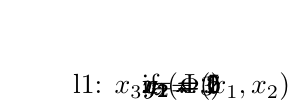
\begin{tikzpicture}
  \node (start) {};
  \node (a) {$x_1 = 5$};
  \node (b) {$x_2 = 6$};
  \node (c) {if ($\ldots$)};
  \node (d) {$y_1 = 1$};
  \node (e) {$y_2 = 2$};
  \node (f) {$z = 3$};
  \node (g) {l1: $x_3 = \Phi(x_1, x_2)$};
  \draw[->] (start) -- (a);
  \draw[->] (start) -- (b);
  \draw[->] (a) -- (g);
  \draw[->] (b) -- (c);
  \draw[->] (c) -- (d);
  \draw[->] (c) -- (e);
  \draw[->] (d) -- (f);
  \draw[->] (e) -- (f);
  \draw[->] (f) -- (g);
\end{tikzpicture}
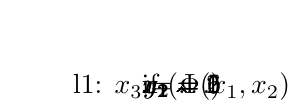
\begin{tikzpicture}
  \node (start) {};
  \node (a) {$x_1 = 5$};
  \node (b) {$x_2 = 6$};
  \node (c) {if ($\ldots$)};
  \node (d) {$y_1 = 1$};
  \node (e) {$y_2 = 2$};
  \node (g) {l1: $x_3 = \Phi(x_1, x_2)$};
  \draw[->] (start) -- (a);
  \draw[->] (start) -- (b);
  \draw[->] (a) -- (g);
  \draw[->] (b) -- (c);
  \draw[->] (c) -- (d);
  \draw[->] (c) -- (e);
  \draw[->] (d) -- (g);
  \draw[->] (e) -- (g);
\end{tikzpicture}
\caption{Optimising an SSA-form machine}
\label{fig:ssa_cfg1}
\end{figure}

\todo{Not actually sure how interesting this is, now that I've written it down.}

\subsection{Building write-side \StateMachines}

Once SLI has obtained the read-side \StateMachine, it can analyse it to determine which loads affect the ultimate prediction, and then compare this set to the dynamic model to determine which stores might potentially influence it.
The analysis must then consider all dynamic paths of $N^w$ instructions which contain at least one of those store operations.
As when building read-side \StateMachines, it would be possible to do this by enumerating all possible such paths and compiling each to an independent \StateMachine, but that would be extremely wasteful.
SLI uses a somewhat more intelligent approach.
The basic approach here is essentially the same as that used for read-side \StateMachines: convert the set of dynamic paths into a (hopefully much smaller) set of acyclic control-flow graphs and then compile those CFGs into \StateMachines.
The details of the algorithms used are, however, slightly different.

\subsubsection{Finding relevant stores}

The first phase of building the write-side \StateMachines is to determine which stores in the program might possibly be relevant.
These are the ones which might affect the result produced by the read-side \StateMachine.
Finding these is straightforward:

\begin{itemize}
\item
  Remove all of the optional annotations from the read-side \StateMachine.
  These are the side effects which provide additional information to the analysis but do not themselves affect the semantics of the \StateMachine, such as assert or stack-layout side effects.
\item
  Simplify the resulting machine down as far as possible.
  Removing annotations can sometimes enable further optimisations if, for instance, two path through the \StateMachine are identical except for inserting an additional intermediate function in the call stack and that intermediate function does not itself perform any relevant operations.
\item
  Find all of the memory load operations which remain the simplified machine.
\item
  Examine the model collected during the dynamic analysis phase to locate all of the stores which might access the same memory location as one of those loads.
  This effectively assumes both that the dynamic analysis phase has correctly captured the program's internal type system and that the program has a particular memory safety property.
  \todo{Say more.}
\end{itemize}

\subsubsection{Build write-side CFGs}
\todo{This has far more pages than it really deserves, although most
  of them are diagrams, so I guess it's not too bad.}

The input to this phase of the analysis is a set of potentially relevant static store instructions, and the analysis must build a collection of acyclic CFGs which cover all possible paths through the program which use at least one of those static instructions and which contain at most $N_w$ instructions.
\editorial{That's not quite the problem definition I used earlier, but it's a bit easier to describe.}

One important assumption here is that the set of potentially relevant store instructions is complete, in the sense that no instruction not in that set can influence the behaviour of the load machine (this follows from the assumption that the dynamic model is itself complete).
This implies that the only parts of the dynamic write path which are actually important are the potentially relevant store instructions; everything else simply acts to constrain the behaviour of those instructions.
That in turn means that it is safe to ignore any prefix or suffix of a dynamic path which does not involve any potentially-relevant store instructions, or, to put it another way, the store CFGs only need to represent dynamic paths which start and end with potentially-relevant instructions.
This is a useful simplification.

The algorithm begins by building a partial static CFG starting at each of the potentially-relevant store instructions and covering every instruction reachable within $N_w$ instructions of that point.
As with read-side CFGs, called functions are effectively inlined into each call site, and returns from the function containing the potentially-relevant store are handled by replacing the instruction with one with a synthesised call stack and restarting.
The CFGs generated by different starting instructions will often overlap; this is handled by sharing nodes between the relevant CFGs.
The resulting CFG is then trimmed to remove any instructions which cannot reach a potentially-relevant store within $N_w$ instructions.

At this point, the CFG represents a fragment of the program and contains every instruction which might be on one of the trimmed dynamic paths which need to be represented by the output CFG, and it only remains to remove any cycles from it.
As with read-side CFGs, this is accomplished by duplicating nodes so as to unroll loops until any path which uses the loop more than once must be longer than $N_w$ instructions and can hence be discarded.
There is, however, one important difference: in the read-side CFG, we are interested in any path which terminates at a specific point, whereas in the write-side CFG we need to preserve any path which starts and ends with any member of a set of interesting instructions.
This makes it more difficult to determine when a loop has been unrolled sufficiently, as it is no longer sufficient to just check the distance to a nominated target instruction.
SLI solves this problem by labelling each node in the graph with information about where it might occur in an interesting path.
This label consists of:

\begin{itemize}
\item
  For each possibly-relevant store, the minimum distance from that store to the labelled node.
\item
  For each possible-relevant store, the minimum distance from the labelled node to that store or any of its duplicates.
\end{itemize}

We only need to consider paths of length $N_w$ or less which start with one of the potentially-relevant stores and which end with a potentially-relevant store or one of its duplicates.
Therefore, if, for any node, the minimum of the first type of label plus the minimum of the second type of label exceeds $N_w$ the node can be safely discarded.
This allows us to break cycles once they have been unrolled far enough.

\begin{algorithmic}
  \STATE {Compute initial labelling of graph}
  \FORALL {$t$ in the set of potentially-relevant stores}
    \WHILE {graph rooted at $t$ is not cycle-free}
       \STATE $edge \gets findEdgeToBeBroken(t, \{\})$
       \STATE $newLabel \gets combineLabels(\text{current label of } edge.start, \text{current label of } edge.end)$
       \IF {$min(newLabel.minFrom) + min(newLabel.minTo) > N_w$}
           \STATE {remove $edge$}
       \ELSE
           \STATE $newNode <- \text{duplicate } edge.end$
           \FORALL {Edges $e$ leaving $edge.end$}
              \STATE {Create a new edge from $newNode$ to $e.end$}
           \ENDFOR
           \STATE {Set label of $newNode$ to $newLabel$}
           \STATE {Replace $edge$ with an edge from $edge.start$ to $newNode$}
       \ENDIF
    \ENDWHILE
  \ENDFOR
\end{algorithmic}

\begin{tikzpicture}
  \node (A) at (0,2) [TrueCfgInstr] {A};
  \node (B) [CfgInstr, below=of A] {B} edge [in=30,out=-30,loop] ();
  \node (C) [TrueCfgInstr, below=of B] {C};
  \draw[->] (A) -- (B);
  \draw[->] (B) -- (C);
  \draw[->] (C) to [bend left=90] (A) node (edge1) [right,midway] {~~~~~~~~};
  \begin{pgfonlayer}{bg}
    \node(box1) [fill=black!10,fit=(A) (B) (C) (edge1)] {};
  \end{pgfonlayer}
  \draw node [right=of box1] {
    \begin{tabular}{lcccc}
      labels & min to A & min from A & min to C & min from C\\
      A & 0 & 0 & 2 & 1\\
      B & 2 & 1 & 1 & 2\\
      C & 1 & 2 & 0 & 0\\
    \end{tabular}
  };
\end{tikzpicture}

\begin{tikzpicture}
  \node (A) at (0,2) [TrueCfgInstr] {A};
  \node (B) [CfgInstr, below=of A] {B};
  \node (B1) [NewCfgInstr, right=of B] {B1};
  \node (C) [TrueCfgInstr, below=of B] {C};
  \draw[->] (A) -- (B);
  \draw[->] (B) -- (C);
  \draw[->] (B) to [bend left=10] (B1);
  \draw[->,swungEdge] (B1) to [bend left=10] (B);
  \draw[->] (B1) -- (C);
  \draw[->] (C) to [bend left=90] (A) node (edge1) [right,midway] {~~~~~~~~};
  \begin{pgfonlayer}{bg}
    \node(box1) [fill=black!10,fit=(A) (B) (B1) (C) (edge1)] {};
  \end{pgfonlayer}
  \draw node [right=of box1] {
    \begin{tabular}{lcccc}
      labels & min to A & min from A & min to C & min from C\\
      A  & 0 & 0 & 2 & 1\\
      B  & 2 & 1 & 1 & 2\\
      C  & 1 & 2 & 0 & 0\\
      B1 & 2 & 2 & 1 & 3\\
    \end{tabular}
    (dupe B)
  };
\end{tikzpicture}

\begin{tikzpicture}
  \node (A) at (0,2) [TrueCfgInstr] {A};
  \node (B) [CfgInstr, below=of A] {B};
  \node (B1) [CfgInstr, right=of B] {B1};
  \node (C) [TrueCfgInstr, below=of B] {C};
  \node (A1) [NewCfgInstr,right=of C] {A1};
  \draw[->] (A) -- (B);
  \draw[->,swungEdge] (A1) -- (B);
  \draw[->] (B) -- (C);
  \draw[->] (B) to [bend left=10] (B1);
  \draw[->] (B1) -- (C);
  \draw[->] (B1) to [bend left=10] (B);
  \draw[->] (C) -- (A1);
  \begin{pgfonlayer}{bg}
    \node(box1) [fill=black!10,fit=(A) (B) (B1) (C) (edge1)] {};
  \end{pgfonlayer}
  \draw node [right=of box1] {
    \begin{tabular}{lcccc}
      labels & min to A & min from A & min to C & min from C\\
      A  & 0 & 0 & 2 & $\infty$\\
      A1 & 0 & 3 & 2 & 1\\
      B  & 2 & 1 & 1 & 2\\
      C  & 1 & 2 & 0 & 0\\
      B1 & 2 & 2 & 1 & 3\\
    \end{tabular}
    (dupe A)
  };
\end{tikzpicture}

\begin{tikzpicture}
  \node (A) at (0,2) [TrueCfgInstr] {A};
  \node (B) [CfgInstr, below=of A] {B};
  \node (B1) [CfgInstr, right=of B] {B1};
  \node (B2) [NewCfgInstr, right=of B1] {B2};
  \node (C) [TrueCfgInstr, below=of B] {C};
  \node (A1) [DupeCfgInstr,right=of C] {A1};
  \draw[->] (A) -- (B);
  \draw[->] (A1) -- (B);
  \draw[->] (B) -- (C);
  \draw[->] (B) -- (B1);
  \draw[->,swungEdge] (B1) to [bend left=10] (B2);
  \draw[->] (B1) -- (C);
  \draw[->] (B2) to [bend left=10] (B1);
  \draw[->] (B2) -- (C);
  \draw[->] (C) -- (A1);
  \begin{pgfonlayer}{bg}
    \node(box1) [fill=black!10,fit=(A) (A1) (B) (B1) (B2) (C) (edge1)] {};
  \end{pgfonlayer}
  \draw node [right=of box1] {
    \begin{tabular}{lcccc}
      labels & min to A & min from A & min to C & min from C\\
      A  & 0 & 0 & 2 & $\infty$\\
      A1 & 0 & 3 & 2 & 1\\
      B  & 2 & 1 & 1 & 2\\
      C  & 1 & 2 & 0 & 0\\
      B1 & 2 & 2 & 1 & 3\\
      B2 & 2 & 3 & 1 & 4\\
    \end{tabular}
  };
\end{tikzpicture}

\begin{tikzpicture}
  \node (A) at (0,2) [TrueCfgInstr] {A};
  \node (B) [CfgInstr, below=of A] {B};
  \node (B1) [CfgInstr, right=of B] {B1};
  \node (B2) [CfgInstr, right=of B1] {B2};
  \node (A1) [DupeCfgInstr,right=of C] {A1};
  \node (C) [TrueCfgInstr, below=of B] {C};
  \node (B3) [NewCfgInstr, below=of A1] {B3};
  \draw[->] (A) -- (B);
  \draw[->,swungEdge] (A1) -- (B3);
  \draw[->] (B) -- (C);
  \draw[->] (B) -- (B1);
  \draw[->] (B1) to [bend left=10] (B2);
  \draw[->] (B1) -- (C);
  \draw[->] (B2) to [bend left=10] (B1);
  \draw[->] (B2) -- (C);
  \draw[->] (B3) -- (C);
  \draw[->] (B3) to [bend right=45] (B1);
  \draw[->] (C) -- (A1);
  \begin{pgfonlayer}{bg}
    \node(box1) [fill=black!10,fit=(A) (A1) (B) (B1) (B2) (B3) (C) (edge1)] {};
  \end{pgfonlayer}
  \draw node [right=of box1] {
    \begin{tabular}{lcccc}
      labels & min to A & min from A & min to C & min from C\\
      A  & 0 & 0 & 2 & $\infty$\\
      A1 & 0 & 3 & 2 & 1\\
      B  & 2 & 1 & 1 & $\infty$\\
      C  & 1 & 2 & 0 & 0\\
      B1 & 2 & 2 & 1 & 3\\
      B2 & 2 & 3 & 1 & 4\\
      B3 & 2 & 4 & 1 & 2\\
    \end{tabular}
  };
\end{tikzpicture}

\begin{tikzpicture}
  \node (A) at (0,2) [TrueCfgInstr] {A};
  \node (B) [CfgInstr, below=of A] {B};
  \node (B1) [CfgInstr, right=of B] {B1};
  \node (B2) [CfgInstr, right=of B1] {B2};
  \node (A1) [DupeCfgInstr,right=of C] {A1};
  \node (C) [TrueCfgInstr, below=of B] {C};
  \node (B3) [CfgInstr, below=of A1] {B3};
  \draw[->] (A) -- (B);
  \draw[->] (A1) -- (B3);
  \draw[->] (B) -- (C);
  \draw[->] (B) -- (B1);
  \draw[->] (B1) to [bend left=10] (B2);
  \draw[->] (B1) -- (C);
  \draw[->] (B2) to [bend left=10] (B1);
  \draw[->,killEdge] (B2) to [bend left=10] (B1);
  \draw[->] (B2) -- (C);
  \draw[->] (B3) -- (C);
  \draw[->] (B3) to [bend right=45] (B1);
  \draw[->] (C) -- (A1);
  \begin{pgfonlayer}{bg}
    \node(box1) [fill=black!10,fit=(A) (A1) (B) (B1) (B2) (B3) (C) (edge1)] {};
  \end{pgfonlayer}
  \draw node [right=of box1] {
    \begin{tabular}{lcccc}
      labels & min to A & min from A & min to C & min from C\\
      A  & 0 & 0 & 2 & $\infty$\\
      A1 & 0 & 3 & 2 & 1\\
      B  & 2 & 1 & 1 & $\infty$\\
      C  & 1 & 2 & 0 & 0\\
      B1 & 2 & 2 & 1 & 3\\
      B2 & 2 & 3 & 1 & 4\\
      New label & 2 & 4 & 1 & 5\\
    \end{tabular}
  };
\end{tikzpicture}

\begin{tikzpicture}
  \node (A) at (0,2) [TrueCfgInstr] {A};
  \node (B) [CfgInstr, below=of A] {B};
  \node (B1) [CfgInstr, right=of B] {B1};
  \node (B2) [CfgInstr, right=of B1] {B2};
  \node (A1) [DupeCfgInstr,right=of C] {A1};
  \node (C) [TrueCfgInstr, below=of B] {C};
  \node (B3) [CfgInstr, below=of A1] {B3};
  \node (C1) [NewCfgInstr, below=of B3] {C1};
  \draw[->] (A) -- (B);
  \draw[->] (A1) -- (B3);
  \draw[->] (B) -- (C);
  \draw[->] (B) -- (B1);
  \draw[->] (B1) -- (B2);
  \draw[->] (B1) -- (C);
  \draw[->] (B2) -- (C);
  \draw[->] (B3) to [bend left=45] (B1);
  \draw[->] (C) -- (A1);
  \draw[->] (C1) to [bend right=90] (A1);
  \draw[->,swungEdge] (B3) -- (C1);
  \begin{pgfonlayer}{bg}
    \node(box1) [fill=black!10,fit=(A) (A1) (B) (B1) (B2) (B3) (C) (C1) (edge1)] {};
  \end{pgfonlayer}
  \draw node [right=of box1] {
    \begin{tabular}{lcccc}
      labels & min to A & min from A & min to C & min from C\\
      A  & 0 & 0 & 2 & $\infty$\\
      A1 & 0 & 3 & 2 & 1\\
      B  & 2 & 1 & 1 & $\infty$\\
      C  & 1 & 2 & 0 & 0\\
      B1 & 2 & 2 & 1 & 3\\
      B2 & 2 & 3 & 1 & 4\\
      C3 & 1 & 4 & 0 & 3\\
    \end{tabular}
  };
\end{tikzpicture}

\begin{tikzpicture}
  \node (A) at (0,2) [TrueCfgInstr] {A};
  \node (B) [CfgInstr, below=of A] {B};
  \node (B1) [CfgInstr, right=of B] {B1};
  \node (B2) [CfgInstr, right=of B1] {B2};
  \node (A1) [DupeCfgInstr,right=of C] {A1};
  \node (C) [TrueCfgInstr, below=of B] {C};
  \node (B3) [CfgInstr, below=of A1] {B3};
  \node (C1) [DupeCfgInstr, below=of B3] {C1};
  \node (B4) [NewCfgInstr, right=of B3] {B4};
  \draw[->] (A) -- (B);
  \draw[->] (A1) -- (B3);
  \draw[->] (B) -- (C);
  \draw[->] (B) -- (B1);
  \draw[->] (B1) -- (B2);
  \draw[->] (B1) -- (C);
  \draw[->] (B2) -- (C);
  \draw[->,swungEdge] (B3) -- (B4);
  \draw[->] (C) -- (A1);
  \draw[->] (C1) to [bend right=45] (A1);
  \draw[->] (B3) -- (C1);
  \draw[->] (B4) -- (C);
  \draw[->] (B4) -- (B2);
  \begin{pgfonlayer}{bg}
    \node(box1) [fill=black!10,fit=(A) (A1) (B) (B1) (B2) (B3) (C) (C1) (edge1)] {};
  \end{pgfonlayer}
  \draw node [right=of box1] {
    \begin{tabular}{lcccc}
      labels & min to A & min from A & min to C & min from C\\
      A  & 0 & 0 & 2 & $\infty$\\
      A1 & 0 & 3 & 2 & 1\\
      B  & 2 & 1 & 1 & $\infty$\\
      C  & 1 & 2 & 0 & 0\\
      B1 & 2 & 2 & 1 & $\infty$\\
      B2 & 2 & 3 & 1 & 4\\
      C3 & 1 & 4 & 0 & 3\\
      B4 & 2 & 5 & 1 & 3\\
    \end{tabular}
  };
\end{tikzpicture}

\begin{tikzpicture}
  \node (A) at (0,2) [TrueCfgInstr] {A};
  \node (B) [CfgInstr, below=of A] {B};
  \node (B1) [CfgInstr, right=of B] {B1};
  \node (B2) [CfgInstr, right=of B1] {B2};
  \node (A1) [DupeCfgInstr,right=of C] {A1};
  \node (C) [TrueCfgInstr, below=of B] {C};
  \node (B3) [CfgInstr, below=of A1] {B3};
  \node (C1) [DupeCfgInstr, below=of B3] {C1};
  \node (B4) [CfgInstr, right=of B3] {B4};
  \node (A2) [NewCfgInstr, left=of C1] {A2};
  \draw[->] (A) -- (B);
  \draw[->] (A1) -- (B3);
  \draw[->] (B) -- (C);
  \draw[->] (B) -- (B1);
  \draw[->] (B1) -- (B2);
  \draw[->] (B1) -- (C);
  \draw[->] (B2) -- (C);
  \draw[->] (B3) -- (B4);
  \draw[->] (C) -- (A1);
  \draw[->,swungEdge] (C1) -- (A2);
  \draw[->] (B3) -- (C1);
  \draw[->] (B4) -- (C);
  \draw[->] (B4) -- (B2);
  \draw[->] (A2) -- (B3);
  \begin{pgfonlayer}{bg}
    \node(box1) [fill=black!10,fit=(A) (A1) (A2) (B) (B1) (B2) (B3) (C) (C1) (edge1)] {};
  \end{pgfonlayer}
  \draw node [right=of box1] {
    \begin{tabular}{lcccc}
      labels & min to A & min from A & min to C & min from C\\
      A  & 0 & 0 & 2 & $\infty$\\
      A1 & 0 & 3 & 2 & 1\\
      B  & 2 & 1 & 1 & $\infty$\\
      C  & 1 & 2 & 0 & 0\\
      B1 & 2 & 2 & 1 & $\infty$\\
      B2 & 2 & 3 & 1 & 4\\
      C3 & 1 & 4 & 0 & 3\\
      B4 & 2 & 5 & 1 & 3\\
      A2 & 0 & 6 & 2 & 4\\
    \end{tabular}
  };
\end{tikzpicture}

\begin{tikzpicture}
  \node (A) at (0,2) [TrueCfgInstr] {A};
  \node (B) [CfgInstr, below=of A] {B};
  \node (B1) [CfgInstr, right=of B] {B1};
  \node (B2) [CfgInstr, right=of B1] {B2};
  \node (A1) [DupeCfgInstr,right=of C] {A1};
  \node (C) [TrueCfgInstr, below=of B] {C};
  \node (B3) [CfgInstr, below=of A1] {B3};
  \node (C1) [DupeCfgInstr, below=of B3] {C1};
  \node (B4) [CfgInstr, right=of B3] {B4};
  \node (A2) [DupeCfgInstr, left=of C1] {A2};
  \node (C2) [NewCfgInstr, below=of B4] {C2};
  \draw[->] (A) -- (B);
  \draw[->] (A1) -- (B3);
  \draw[->] (B) -- (C);
  \draw[->] (B) -- (B1);
  \draw[->] (B1) -- (B2);
  \draw[->] (B1) -- (C);
  \draw[->] (B2) -- (C);
  \draw[->] (B3) -- (B4);
  \draw[->] (C) -- (A1);
  \draw[->] (C1) -- (A2);
  \draw[->] (B3) -- (C1);
  \draw[->,swungEdge] (B4) -- (C2);
  \draw[->] (B4) -- (B2);
  \draw[->] (A2) -- (B3);
  \draw[->] (C2) -- (A1);
  \begin{pgfonlayer}{bg}
    \node(box1) [fill=black!10,fit=(A) (A1) (A2) (B) (B1) (B2) (B3) (C) (C1) (C2) (edge1)] {};
  \end{pgfonlayer}
  \draw node [right=of box1] {
    \begin{tabular}{lcccc}
      labels & min to A & min from A & min to C & min from C\\
      A  & 0 & 0 & 2 & $\infty$\\
      A1 & 0 & 3 & 2 & 1\\
      B  & 2 & 1 & 1 & $\infty$\\
      C  & 1 & 2 & 0 & 0\\
      B1 & 2 & 2 & 1 & $\infty$\\
      B2 & 2 & 3 & 1 & 4\\
      C3 & 1 & 4 & 0 & 3\\
      B4 & 2 & 5 & 1 & 3\\
      A2 & 0 & 6 & 2 & 4\\
      C2 & 1 & 6 & 0 & 4\\
    \end{tabular}
  };
\end{tikzpicture}

\begin{tikzpicture}
  \node (A) at (0,2) [TrueCfgInstr] {A};
  \node (B) [CfgInstr, below=of A] {B};
  \node (B1) [CfgInstr, right=of B] {B1};
  \node (B2) [CfgInstr, right=of B1] {B2};
  \node (A1) [DupeCfgInstr,right=of C] {A1};
  \node (C) [TrueCfgInstr, below=of B] {C};
  \node (B3) [CfgInstr, below=of A1] {B3};
  \node (C1) [DupeCfgInstr, below=of B3] {C1};
  \node (B4) [CfgInstr, right=of B3] {B4};
  \node (A2) [DupeCfgInstr, left=of C1] {A2};
  \node (C2) [DupeCfgInstr, below=of B4] {C2};
  \draw[->] (A) -- (B);
  \draw[->] (A1) -- (B3);
  \draw[->] (B) -- (C);
  \draw[->] (B) -- (B1);
  \draw[->] (B1) -- (B2);
  \draw[->] (B1) -- (C);
  \draw[->] (B2) -- (C);
  \draw[->] (B3) -- (B4);
  \draw[->] (C) -- (A1);
  \draw[->] (C1) -- (A2);
  \draw[->] (B3) -- (C1);
  \draw[->] (B4) -- (C2);
  \draw[->] (B4) -- (B2);
  \draw[->] (A2) -- (B3);
  \draw[->,killEdge] (A2) -- (B3);
  \draw[->] (C2) -- (A1);
  \begin{pgfonlayer}{bg}
    \node(box1) [fill=black!10,fit=(A) (A1) (A2) (B) (B1) (B2) (B3) (C) (C1) (C2) (edge1)] {};
  \end{pgfonlayer}
  \draw node [right=of box1] {
    \begin{tabular}{lcccc}
      labels & min to A & min from A & min to C & min from C\\
      A  & 0 & 0 & 2 & $\infty$\\
      A1 & 0 & 3 & 2 & 1\\
      B  & 2 & 1 & 1 & $\infty$\\
      C  & 1 & 2 & 0 & 0\\
      B1 & 2 & 2 & 1 & $\infty$\\
      B2 & 2 & 3 & 1 & 4\\
      C3 & 1 & 4 & 0 & 3\\
      B4 & 2 & 5 & 1 & 3\\
      A2 & 0 & 6 & 2 & 4\\
      C2 & 1 & 6 & 0 & 4\\
      New label & 2 & 7 & 1 & 5\\
    \end{tabular}\\
    (Dupe B5)
  };
\end{tikzpicture}

\begin{tikzpicture}
  \node (A) at (0,2) [TrueCfgInstr] {A};
  \node (B) [CfgInstr, below=of A] {B};
  \node (B1) [CfgInstr, right=of B] {B1};
  \node (B2) [CfgInstr, right=of B1] {B2};
  \node (A1) [DupeCfgInstr,right=of C] {A1};
  \node (C) [TrueCfgInstr, below=of B] {C};
  \node (B3) [CfgInstr, below=of A1] {B3};
  \node (C1) [DupeCfgInstr, below=of B3] {C1};
  \node (B4) [CfgInstr, right=of B3] {B4};
  \node (A2) [DupeCfgInstr, left=of C1] {A2};
  \node (C2) [DupeCfgInstr, below=of B4] {C2};
  \draw[->] (A) -- (B);
  \draw[->] (A1) -- (B3);
  \draw[->] (B) -- (C);
  \draw[->] (B) -- (B1);
  \draw[->] (B1) -- (B2);
  \draw[->] (B1) -- (C);
  \draw[->] (B2) -- (C);
  \draw[->] (B3) -- (B4);
  \draw[->] (C) -- (A1);
  \draw[->] (C1) -- (A2);
  \draw[->] (B3) -- (C1);
  \draw[->] (B4) -- (C2);
  \draw[->] (B4) -- (B2);
  \draw[->] (C2) -- (A1);
  \draw[->,killEdge] (C2) -- (A1);
  \begin{pgfonlayer}{bg}
    \node(box1) [fill=black!10,fit=(A) (A1) (A2) (B) (B1) (B2) (B3) (C) (C1) (C2) (edge1)] {};
  \end{pgfonlayer}
  \draw node [right=of box1] {
    \begin{tabular}{lcccc}
      labels & min to A & min from A & min to C & min from C\\
      A  & 0 & 0 & 2 & $\infty$\\
      A1 & 0 & 3 & 2 & 1\\
      B  & 2 & 1 & 1 & $\infty$\\
      C  & 1 & 2 & 0 & 0\\
      B1 & 2 & 2 & 1 & $\infty$\\
      B2 & 2 & 3 & 1 & 4\\
      C3 & 1 & 4 & 0 & 3\\
      B4 & 2 & 5 & 1 & 3\\
      A2 & 0 & 6 & 2 & 4\\
      C2 & 1 & 6 & 0 & 4\\
      New label & 0 & 7 & 2 & 5\\
    \end{tabular}\\
    (Dupe A1)
  };
\end{tikzpicture}

\begin{tikzpicture}
  \node (A) at (0,2) [TrueCfgInstr] {A};
  \node (B) [CfgInstr, below=of A] {B};
  \node (B1) [CfgInstr, right=of B] {B1};
  \node (B2) [CfgInstr, right=of B1] {B2};
  \node (A1) [DupeCfgInstr,right=of C] {A1};
  \node (C) [TrueCfgInstr, below=of B] {C};
  \node (B3) [CfgInstr, below=of A1] {B3};
  \node (C1) [DupeCfgInstr, below=of B3] {C1};
  \node (B4) [CfgInstr, right=of B3] {B4};
  \node (A2) [DupeCfgInstr, left=of C1] {A2};
  \node (C2) [DupeCfgInstr, below=of B4] {C2};
  \node (C3) [NewCfgInstr, right=of A1] {C3};
  \draw[->] (A) -- (B);
  \draw[->] (A1) -- (B3);
  \draw[->] (B) -- (C);
  \draw[->] (B) -- (B1);
  \draw[->] (B1) -- (B2);
  \draw[->] (B1) -- (C);
  \draw[->,swungEdge] (B2) -- (C3);
  \draw[->] (B3) -- (B4);
  \draw[->] (C) -- (A1);
  \draw[->] (C1) -- (A2);
  \draw[->] (B3) -- (C1);
  \draw[->] (B4) -- (C2);
  \draw[->] (B4) to [bend left=45] (B2);
  \draw[->] (C3) -- (A1);
  \begin{pgfonlayer}{bg}
    \node(box1) [fill=black!10,fit=(A) (A1) (A2) (B) (B1) (B2) (B3) (C) (C1) (C2) (C3) (edge1)] {};
  \end{pgfonlayer}
  \draw node [right=of box1] {
    \begin{tabular}{lcccc}
      labels & min to A & min from A & min to C & min from C\\
      A  & 0 & 0 & 2 & $\infty$\\
      A1 & 0 & 3 & 2 & 1\\
      B  & 2 & 1 & 1 & $\infty$\\
      C  & 1 & 2 & 0 & 0\\
      B1 & 2 & 2 & 1 & $\infty$\\
      B2 & 2 & 3 & 1 & 4\\
      C3 & 1 & 4 & 0 & 3\\
      B4 & 2 & 5 & 1 & 3\\
      A2 & 0 & 6 & 2 & 4\\
      C2 & 1 & 6 & 0 & 4\\
      C3 & 1 & 4 & 0 & 5\\
    \end{tabular}
  };
\end{tikzpicture}

\begin{tikzpicture}
  \node (A) at (0,2) [TrueCfgInstr] {A};
  \node (B) [CfgInstr, below=of A] {B};
  \node (B1) [CfgInstr, right=of B] {B1};
  \node (B2) [CfgInstr, right=of B1] {B2};
  \node (A1) [DupeCfgInstr,right=of C] {A1};
  \node (C) [TrueCfgInstr, below=of B] {C};
  \node (B3) [CfgInstr, below=of A1] {B3};
  \node (C1) [DupeCfgInstr, below=of B3] {C1};
  \node (B4) [CfgInstr, right=of B3] {B4};
  \node (A2) [DupeCfgInstr, left=of C1] {A2};
  \node (C2) [DupeCfgInstr, below=of B4] {C2};
  \node (C3) [DupeCfgInstr, right=of A1] {C3};
  \draw[->] (A) -- (B);
  \draw[->] (A1) -- (B3);
  \draw[->] (B) -- (C);
  \draw[->] (B) -- (B1);
  \draw[->] (B1) -- (B2);
  \draw[->] (B1) -- (C);
  \draw[->] (B2) -- (C3);
  \draw[->] (B3) -- (B4);
  \draw[->] (C) -- (A1);
  \draw[->] (C1) -- (A2);
  \draw[->] (B3) -- (C1);
  \draw[->] (B4) -- (C2);
  \draw[->] (B4) to [bend left=45] (B2);
  \draw[->,killEdge] (B4) to [bend left=45] (B2);
  \draw[->] (C3) -- (A1);
  \begin{pgfonlayer}{bg}
    \node(box1) [fill=black!10,fit=(A) (A1) (A2) (B) (B1) (B2) (B3) (C) (C1) (C2) (C3) (edge1)] {};
  \end{pgfonlayer}
  \draw node [right=of box1] {
    \begin{tabular}{lcccc}
      labels & min to A & min from A & min to C & min from C\\
      A  & 0 & 0 & 2 & $\infty$\\
      A1 & 0 & 3 & 2 & 1\\
      B  & 2 & 1 & 1 & $\infty$\\
      C  & 1 & 2 & 0 & 0\\
      B1 & 2 & 2 & 1 & $\infty$\\
      B2 & 2 & 3 & 1 & $\infty$\\
      C3 & 1 & 4 & 0 & $\infty$\\
      B4 & 2 & 5 & 1 & 3\\
      A2 & 0 & 6 & 2 & 4\\
      C2 & 1 & 6 & 0 & 4\\
      C3 & 1 & 4 & 0 & 5\\
      New label & 2 & 6 & 1 & 4\\
    \end{tabular}
  };
\end{tikzpicture}

\begin{tikzpicture}
  \node (A) at (0,2) [TrueCfgInstr] {A};
  \node (B) [CfgInstr, below=of A] {B};
  \node (B1) [CfgInstr, right=of B] {B1};
  \node (B2) [CfgInstr, right=of B1] {B2};
  \node (A1) [DupeCfgInstr,right=of C] {A1};
  \node (C) [TrueCfgInstr, below=of B] {C};
  \node (B3) [CfgInstr, below=of A1] {B3};
  \node (C1) [DupeCfgInstr, below=of B3] {C1};
  \node (B4) [CfgInstr, right=of B3] {B4};
  \node (A2) [DupeCfgInstr, left=of C1] {A2};
  \node (C2) [DupeCfgInstr, below=of B4] {C2};
  \node (C3) [DupeCfgInstr, right=of A1] {C3};
  \draw[->] (A) -- (B);
  \draw[->] (A1) -- (B3);
  \draw[->] (B) -- (C);
  \draw[->] (B) -- (B1);
  \draw[->] (B1) -- (B2);
  \draw[->] (B1) -- (C);
  \draw[->] (B2) -- (C3);
  \draw[->] (B3) -- (B4);
  \draw[->] (C) -- (A1);
  \draw[->] (C1) -- (A2);
  \draw[->] (B3) -- (C1);
  \draw[->] (B4) -- (C2);
  \draw[->] (C3) -- (A1);
  \draw[->,killEdge] (C3) -- (A1);
  \begin{pgfonlayer}{bg}
    \node(box1) [fill=black!10,fit=(A) (A1) (A2) (B) (B1) (B2) (B3) (C) (C1) (C2) (C3) (edge1)] {};
  \end{pgfonlayer}
  \draw node [right=of box1] {
    \begin{tabular}{lcccc}
      labels & min to A & min from A & min to C & min from C\\
      A  & 0 & 0 & 2 & $\infty$\\
      A1 & 0 & 3 & 2 & 1\\
      B  & 2 & 1 & 1 & $\infty$\\
      C  & 1 & 2 & 0 & 0\\
      B1 & 2 & 2 & 1 & $\infty$\\
      B2 & 2 & 3 & 1 & $\infty$\\
      C3 & 1 & 4 & 0 & $\infty$\\
      B4 & 2 & 5 & 1 & 3\\
      A2 & 0 & 6 & 2 & 4\\
      C2 & 1 & 6 & 0 & 4\\
      C3 & 1 & 4 & 0 & 5\\
      New label & 0 & 5 & 2 & 6\\
    \end{tabular}
  };
\end{tikzpicture}

\begin{tikzpicture}
  \node (A) at (0,2) [TrueCfgInstr] {A};
  \node (B) [CfgInstr, below=of A] {B};
  \node (B1) [CfgInstr, right=of B] {B1};
  \node (B2) [CfgInstr, right=of B1] {B2};
  \node (A1) [DupeCfgInstr,right=of C] {A1};
  \node (C) [TrueCfgInstr, below=of B] {C};
  \node (B3) [CfgInstr, below=of A1] {B3};
  \node (C1) [DupeCfgInstr, below=of B3] {C1};
  \node (B4) [CfgInstr, right=of B3] {B4};
  \node (A2) [DupeCfgInstr, left=of C1] {A2};
  \node (C2) [DupeCfgInstr, below=of B4] {C2};
  \node (C3) [DupeCfgInstr, right=of A1] {C3};
  \draw[->] (A) -- (B);
  \draw[->] (A1) -- (B3);
  \draw[->] (B) -- (C);
  \draw[->] (B) -- (B1);
  \draw[->] (B1) -- (B2);
  \draw[->] (B1) -- (C);
  \draw[->] (B2) -- (C3);
  \draw[->] (B3) -- (B4);
  \draw[->] (C) -- (A1);
  \draw[->] (C1) -- (A2);
  \draw[->] (B3) -- (C1);
  \draw[->] (B4) -- (C2);
  \begin{pgfonlayer}{bg}
    \node(box1) [fill=black!10,fit=(A) (A1) (A2) (B) (B1) (B2) (B3) (C) (C1) (C2) (C3) (edge1)] {};
  \end{pgfonlayer}
  \draw node [right=of box1] {
    \begin{tabular}{lcccc}
      labels & min to A & min from A & min to C & min from C\\
      A  & 0 & 0 & 2 & $\infty$\\
      A1 & 0 & 3 & 2 & 1\\
      B  & 2 & 1 & 1 & $\infty$\\
      C  & 1 & 2 & 0 & 0\\
      B1 & 2 & 2 & 1 & $\infty$\\
      B2 & 2 & 3 & 1 & $\infty$\\
      C3 & 1 & 4 & 0 & $\infty$\\
      B4 & 2 & 5 & 1 & 3\\
      A2 & 0 & 6 & 2 & 4\\
      C2 & 1 & 6 & 0 & 4\\
      C3 & 1 & 4 & 0 & 5\\
    \end{tabular}
  };
\end{tikzpicture}


\subsection{Converting pairs of \StateMachines into verification conditions}

We now convert the pair of \StateMachines into a form of verification condition; that is, a predicate on the program's state which is satisfiable when the program contains a bug of the type being investigated\editorial{That isn't quite the usual definition of a verification condition.}.
SLI's completeness property is that if every possible \StateMachine pair which could be generated by the above algorithm is generated and each one is successfully converted to a verification condition (i.e. no part of the analysis times out), and none of the verification conditions are satisfiable, and the dynamic analysis is complete, the program will not contain any bugs of the class being investigated.

At a high level, the verification conditions are produced by considering each of the clauses of the bug definition in section~\todo{...} in turn, converting each into a \StateMachine, and then using symbolic execution to build a predicate saying when that clause might be satisfied.
These clause-conditions are then combined to produce the final verification condition for the original \StateMachine pair.

The rules for building each clause-condition are as follows:

\begin{itemize}
\item P valid -- \editorial{not sure what I'm going to say here -- P doesn't really exist at this stage, so this clause doesn't really make sense here.}
\item R valid -- true by construction of read machine, so the clause condition is just $1$.
\item W valid -- true by construction of write machine, so the clause condition is just $1$.
\item
  R atomic -- this rule states that the read \StateMachine must predict survival when run atomically.
  The \StateMachine to symbolically execute is then just the read-side \StateMachine, and the clause constraint is the rule which the symbolic executor derives for when the \StateMachine will survive.
\item
  W atomic -- this rule states that running the read \StateMachine after the write one must also predict survival.
  For this clause, we symbolically execute the concatenation of the two \StateMachines, and again the clause constraint is the rule when the \StateMachine will survive.
\item
  Crash possible -- this rule states that running the read and write \StateMachines in parallel must sometimes predict a crash.
  For this clause, we symbolically execute the cross-product parallel composition of the two \StateMachines.
  This time, the clause constraint is the rule for when the \StateMachine will crash.
\item
  W isolation -- used extensively when deriving write machine, to the extent that there's rarely any additional useful information to extract by this stage in the pipeline.
\item
  Concurrent -- model of program isn't strong enough to say anything useful about it.
\end{itemize}

We therefore produce three clause constraints for each \StateMachine pair, and must report a bug if they are simultaneously satisfiable.
As a minor optimisation, SLI assumes the R atomic clause is true when deriving the W atomic and crash clauses, and assumes that the W atomic clause is true when deriving the crash possible clause.

\subsubsection{Symbolically executing machines}

SLI uses a simple symbolic execution engine to evaluate machines and
determine when \StateMachines will crash.  The details of this are
fairly standard, and I only give a brief overview
here\editorial{\emph{Should} only give a brief overview; this ended up
  much more detailed than I'd expected.}.  The core data structure
used by the execution engine is a queue of (mostly) symbolic
configurations which the \StateMachine might occupy, and the main
operation is to take a state out of this queue, determine what the
\StateMachine might do next, and possibly add some additional
configurations to the queue to explore further.  Each configuration
contains:

\begin{itemize}
\item
  A mapping from temporary variable identifiers to the (symbolic) values of those variables.
\item
  A reference to the {\StateMachine}'s current (non-symbolic) state.
\item
  The order in which those temporaries were assigned to.
  As discussed in \S~\ref{sect:ssa}, SLI uses a slightly unusual form of single static assignment in which $\Phi$ nodes select their input variable based on which was assigned to most recently, rather than based on the preceding control flow, and this keeping track of that ordering allows that semantics to be implemented simply.
\item
  A log of all of the memory stores issued by the \StateMachine so far.
\item
  The current assumption.
  This is simply the conjunction of all of the conditions which are known to be true at this point in the execution.
\item
  The current ``path'' assumption.
  This is the subset of the current assumption which was introduced during the machine's execution.
  In other words, it is all of the things which are known to be true at this point in the execution but which were not known to be true at the start of the execution.
  This is often useful when building verification conditions, as discussed below.

  An alternative design would instead keep the path assumption and the initial assumption completely separate, and get rid of the current assumption, but this is slightly more convenient\editorial{think harder.}.
\end{itemize}\editorial{Plus some debug crap, but we don't care about that here.}

There are three possible outcomes from an execution: crash, survive, or escape.
The first two are obvious.
An escaping result indicates that the \StateMachine behaved in a way which indicates that this execution is not one of the ones which are of interest to the current bug.
This might, for instance, be because an assertion fails, or because a memory access (other than the one being investigated) dereferenced bad memory.
The exact treatment of escaping executions depends on how the results of the symbolic execution are to be used.

Implementing the various types of \StateMachine operation is straightforward:

\begin{itemize}
\item[cond]
  Check whether the assumption allows the condition to be simplified to a constant.
  If it does, simplify advance to the appropriate successor state.
  Otherwise, create two new successor configurations, moving one to the state's condition-true successor state and the other to the condition-false one and adding either the constraint (for the condition-true successor) or its inverse (for the condition-false one) to the current assumption and the path assumption.
\item[assert]
  Check whether the assumption allows the asserted value to be reduced to a constant.
  If it can, and that constant is one, simply move to the assertion's successor state.
  If the constant is zero, the execution escapes.
  Otherwise, if the asserted expression cannot be reduced to a constant, it is added to the current assumption and path assumption and the execution moves to the successor state.
\item[copy]
  Simplify the right-hand side of the copy as far as possible using the current assumption and then copy it to the appropriate place in the temporary variable table.
  The current assumption is then rewritten to replace any instances of the left-hand side of the copy with the simplified version of the right-hand side.
  The path assumption is not rewritten, and neither are the values of any of the other temporary values.
  \todo{I'm at least half convinced that this doesn't actually matter any more, due to changes elsewhere in the analysis pipeline.  Need to check that.}
\item[store]
  Assert that the pointer stored to is itself valid and then add the store to the log of issued stores.
\item[load]
  Assert that the pointer to be loaded is itself valid.
  Look through the log of issued stores, checking each one to see whether it might be storing to the location loaded by the load.
  If the load is unambiguously satisfied by a single store then create a single successor configuration then copy the value stored into the temporary variable targeted by the load using the same mechanism as used for copy side-effects.
  Otherwise, create one for each possible store, and potentially also one in which the load returns the initial value of memory.
\item[phi]
  Essentially as far copy operations.
\item
  Every operation is a no-op in the interpreter and simply moves to the next state.
  In particular, the execution engine ignores operations such as ``StartLayout'' and ``PointerAliasing'' which simply provide additional hints to the various \StateMachine simplification phases.
\end{itemize}

\todo{Possibly important that this uses the simplifier rather than the sat checker to see whether things reduce to a constant.}

Asserting that pointers are valid before performing memory operations is perhaps slightly surprising, as it means that the execution engine will never consider paths which crash due to dereferencing bad pointers.
This may appear odd in a system designed to investigate crashes due to dereferencing bad pointers.
However, it simply reflects the fact that, at this stage, SLI is only interested in a single possibly-crashing instruction, and so crashes at memory accesses prior to that one need to be ignored; asserting that dereferenced pointers are valid achieves that.
The interesting instruction itself is encoded without an explicit memory-accessing state (see \S~\todo{...}), so crashes there will not be affected by these assertions.

\todo{At one point, the execution engine was the reason we needed dynamic single assignment form.  I can't really see why it depends on it now, though, so that might be worth looking at more.}

\subsubsection{R atomic}

This rule states that the read machine must run to completion without crashing if run in isolation.
Once the read machine has been completely determined, this is in effect a condition on the states of the program which have to be considered: if the read machine would crash when run atomically in state S, any concurrency-related bugs detected starting from state S are highly unlikely to be interesting.
The first phase of building the verification condition is to build the condition.
To do so, the analysis first simplifies the probe machine on the assumption that it is running atomically and then symbolically executes it.
The constraint is then the conjunction of the inverses of the path conditions to reach crashing states.
Escaping executions are treated as crashing ones at this stage, so that they will not be considered by later stages of the analysis.

Path explosion: once you're assuming that the machine is completely atomic the state machine simplifier turns most machines into a simple predicate on the initial state and so the symbolic execution is pretty much trivial and there aren't really any paths to explode.
The main exception is where Phi nodes prevent us from simplifying control flow as far as we'd like.
Aliasing can also be an issue, but much less often than you'd expect.

\subsection{W atomic}

This rule requires that the read machine does not crash if run after the write machine has completed.
This, again, is about restricting the analysis to only consider bugs which are due to concurrency, and not any crashes which might be caused by other bugs.
For this rule, the analysis first concatenates the two machines by replacing the terminal states of the write machine with the first state in the read machine.
The resulting machine is then simplified and interpreted.
In this case, the symbolic execution engine is allowed to assume that the R atomic condition holds while performing this interpretation
The resulting path conditions are converted into a validity predicate in essentially the same way as they are for the R atomic rule.

Path explosion: again modest at this stage.
Most store machines just consist of a small number of store instructions (usually one, almost never more than three) and no control flow, and so we're effectively repeating the R atomic calculations in a slightly different initial state.
The aliasing problems are more complicated here but generally still not intractable.

\subsection{Crash possible}

This rule requires that the read machine must sometimes crash if run in parallel with the store machine.
To build this predicate, the analysis builds a new \StateMachine which is the cross product of the input read and write machines and then interprets that.
For this interpretation, escaping states, where assertions fail, are assumed to survive.
The final result is the disjunction of all of the path conditions which reach crashing states; combined with the validity condition, this describes all of the states which might exhibit a bug of the target class.

Complication: we arrange to build the machines in a way which avoids running either machine to completion in isolation.

I'm going to have to describe the algorithm here, because it's a little bit subtle.

Interesting properties of the algorithm:

\begin{itemize}
\item
  Needs to maintain atomic blocks.
\item
  Need to avoid considering the cases where either machine runs to completion before the other one starts.
\item
  Avoid considering both orderings of a load-store pair if they can't ever possibly access the same memory location.
  Slight complication: need to look past the current memory access to see if there's anything after it which might possibly race in an interesting way.
\item
  When you do need to consider both orderings, one of the orderings asserts that the two accesses access the same location and the other one doesn't.
\end{itemize}

Path explosion: much more of a concern now.
The cross machine will only have $O(n.m)$ states, which isn't \emph{too} bad, but once you combine that with the potential exponential blow-up in the execution engine proper's alias analysis it gets really quite messy.
You save a little because the validity predicate eliminates a bunch of possible configurations, though.

\subsection{Use of the induction rule}

The analysis uses a form of induction to eliminate some bugs.
The idea is that when analysing target instruction T, we can assume that there are no bugs of the target class for any other instruction T', and hence that the verification condition for T' is false.
Therefore, once we've finished generating the verification condition for a \StateMachine pair (L,S) we look at ``truncations'' of $L$, produced by cutting it off at each intermediate memory access, and generate verification conditions for each of them.
We can safely assume that these conditions are false while checking for satisfiability of the verification condition for the original \StateMachine pair.
This relies on the monotonicity property of the definition of crashes discussed in \S~\ref{sect:monotonicity}.

If this eliminates a crash then we log the fact that we've used induction, and then once every instruction has been completed we go back and check for cycles in this induction graph.
Usually, there aren't any, and so the induction is sound.
Otherwise, we count each such cycle as a single bug.

\todo{This isn't particularly effective, and it is very computationally expensive.}

\todo{Haven't actually found any cycles in that graph yet...}

\subsection{Completeness}
This is going to have a lot of forward references, because so many of the potential sources of uncompleteness are in the simplification bits, which I describe much later.

\subsection{Canonicalising machines}

The crash summaries generated by this analysis often contain a lot of redundant information, and this complicates later analysis, and also makes manually reviewing the generated summaries quite difficult.
SLI therefore implements some canonicalisation passes which remove some of this redundancy.

\todo{Caution, brain dump ahead}

\subsection{Phase 1 canonicalisation}
\subsubsection{Aliasing canonicalisation}
The aliasing table is converted into a predicate on the addresses accessed by the various memory accessing instructions and then added to the verification condition.

\subsubsection{Splitting SSA variables}
Two generations of a single SSA variable can be treated as independent variables provided that they're never used in the same $\Phi$ node.
This has no directly useful effects on any of the analyses which we perform, but it makes it a bit easier to canonicalise things.
In effect, this converts the machine part-way back out of SSA form.

\subsubsection{Thread ID canonicalisation}
\todo{Not worth mentioning}
The IDs of threads have no meaning beyond a simple equality test.
Therefore, if a single summary involves threads 1 and 3, but not thread 2, thread 3 could be renamed to thread 2 without it having any semantic effects.
Assigning thread IDs deterministically to members of the crash summary increases canonical-ness.

\subsubsection{Register canonicalisation}
Likewise, register identifiers are pretty much arbitrary, and differences which can be expressed by simple alpha conversion are generally not very interesting.
We therefore rename them in a way which is deterministic given the structure of the summary.
\todo{Analogy with De Bruijn indices?}

\subsubsection{CFG canonicalisation}
\todo{Should really do this, but don't.}

\subsection{Phase 2 canonicalisation}
The \StateMachines generated by the analysis can include some information which is helpful to the analysis but not usually directly relevant to understanding the bug which is being described.
The main examples are start and end of function markers and assertions.
For instance, suppose that the program looks like this:

\begin{verbatim}
f1() {
    if (complicated_condition1)
        return;
    g()
}
f2() {
    if (complicated_condition2)
        return;
    g()
}
\end{verbatim}

And that the \StateMachine for \verb|g| is \verb|g'|.
The state machines for $f1$ and $f2$ might then be:

\begin{verbatim}
f1: Assert (!complicated_condition1)
    g'
f2: Assert (!complicated_condition2)
    g'
\end{verbatim}

It is useful to retain \verb|complicated_condition1| and \verb|complicated_condition2| while generating the summaries, because they may contain information important to the bug, but once the summaries have been generated they become much less useful.
At this point, the only effect of the assertions is to make summaries which would otherwise be identical look like they are different.
Assertions are therefore removed completely during summary canonicalisation.

Likewise, function start and end markers are only used to determine when on-stack variables become live and dead, which is useful during analysis but becomes redundant once the full aliasing table is available.
They are therefore removed at this stage.

\subsection{Phase 3 canonicalisation}

Something about load canonicalisation, and why it has to be reversed later?

Important thing to worry about here is satisfiability of verification condition.

\subsubsection{Equality substitution}
Find equality constraints in the verification condition and use them to eliminate register from the summary.
This is done even when the result is more ``complex'' than the original input summary.
Approach is to find all of the registers which we can eliminate, then pick the one which occurs most often and eliminate it, then repeat until we can't eliminate anything else.

\todo{Need to come up with a coherent explanation of why doing this during analysis is bad.  Experimentally, it is, but it's not entirely obvious why that should be so.}

\subsubsection{Assume that the machines survive when run in isolation}
The verification condition includes the R atomic and W atomic assumptions.
These are necessary for the analysis to be valid, but tend not to provide a great deal of useful information.
This canonicalisation phase removes those components of the condition.
It re-derives the R atomic and W atomic assumptions as conditions, and then simplifies the verification condition and the \StateMachines under the assumption that they hold.

\subsubsection{Removal of redundant clauses}
The verification condition can sometimes include constraints on registers and memory locations which do not occur anywhere in any of the \StateMachines, usually because the \StateMachines have been simplified after the relevant part of the condition was derived.
In the simplest case, these variables are completely independent of the interesting variables.
\todo{Interesting variables are those which appear, or might appear (e.g. LD aliasing), in the \StateMachines.}
To find these, convert the verification condition to conjunctive normal form and then draw a graph whose nodes are variables and which has an edge between A and B if there is any clause in the verification condition which mentions both A and B.
Now find the connected components in this graph, $C_i$.
The verification condition can then be written as $f_1(C_1) \wedge f_2(C_2) \ldots$.
If any of the $C_i$ don't mention any variables in the interesting set then $f_i(C_i)$ can be set to true and hence discarded.

This is safe if $f_i(C_i)$ is satisfiable, which is the common case anyway.

\subsubsection{Removal of underspecified clauses}

If a free variable (i.e. one which isn't mentioned in the \StateMachines) occurs in precisely one place in the verification condition then it is referred to as being underspecified.
This means that, from the point of view of satisfiability checking, it can be set to anything at all, without reference to the rest of verification condition, which in turn means that certain clauses can become trivially satisfiable.
For instance, if $x$ is underspecified in this sense, and the verification condition includes the clause $x == y$, then a satisfiability checker would be able to select an $x$ to make that either true or false, and so our simplifications can assume that $x == y$ is either true or false according to whatever happens to be most convenient in context.

\subsubsection{Functionalisation/conditional independence}

This is analogous to the SSA transformation, but for boolean expressions rather than for programs.
The idea is that if you have a function of two free variables $f(x, y)$, you can treat $y$ as a function of $x$ to get $f(x, y_x)$
If $x$ and $y$ are boolean variables then you can then do a case split on $x$ to get $(x \wedge f(T, y_T)) \vee (\not{}x \wedge f(F, y_F))$.
$y_F$ and $y_T$ are then separate variables, and the two $f$ cases can be subjected to redundant clause removal and underspecified clause removal independently.

\todo{This is in dire need of an example.}

\todo{This is a lot like re-encoding the program's control flow into the verification condition, but in a way which is kind-of minimal and only contains the bits of control flow which are actually relevant.}

\subsection{Phase 4 canonicalisation}
The compound functions stuff.
Essentially, this notices if you have a lot of places in the verification condition/\StateMachine where you go $f(x, 5, 7)$, where $f$ is complex and only $x$ changes, and invents a new function to represent $f(..., 5, 7)$ and does a kind of backwards $\eta$ conversion to get rid of them.

\section{Building crash enforcement plans}

The previous phase of the algorithm produces a set of crash summaries, each of which consists of a read \StateMachine, a write \StateMachine, a verification condition, and an unrolled fragment of the program's control-flow graph.
Each summary is considered in turn and converted into a crash enforcement plan which, when applied to the program, will make the relevant bug more likely to reproduce.
We now illustrate the basic approach with a simple example before giving details of the algorithms used.

Suppose that the bug to be exhibited involves two threads:

\begin{verbatim}
int *global_ptr[];
void thread1(int idx1) {
    if (global_ptr[idx1])
        *global_ptr[idx1] = 7;
} 
void thread2(int idx2) {
    global_ptr[idx2] = NULL;
}
\end{verbatim}

Suppose further that these functions compile to this machine code:

\begin{verbatim}
thread1:

l1:   ADD global_ptr + idx1 -> reg1
l2:   LOAD *reg1 -> reg2
l3:   CMP 0, reg2
l4:   jmp_if_eq l7
l5:   LOAD *reg1 -> reg3
l6:   STORE 7 -> *reg3
l7:

thread2:

l8:   ADD global_ptr + idx2 -> reg4
l9:   STORE 0 -> *reg4
\end{verbatim}

There is a risk here that \verb|thread1| might crash if \verb|l9| is interleaved between \verb|l2| and \verb|l5| and \verb|idx1 == idx2|.
The previous analysis phase will produce \StateMachines something like these:

\begin{tikzpicture}
  \node[stateSideEffect,initial] (l2) {l2: Load $global\_ptr + idx1$ to $tmp1$};
  \node[stateIf,below = of l2] (l4) {l4: If $tmp1 == 0$?};
  \node[stateSideEffect, below = of l4] (l5) {l5: Load $global\_ptr + idx1$ to $tmp2$};
  \node[stateIf,below = of l5] (l6) {If $BadPtr(tmp2)$?};
  \node[stateTerminal,below right = of l6] (crash) {Crash};
  \node[stateTerminal,below left = of l6] (survive) {Survive};
  \draw[->] (l2) -- (l4);
  \draw[->] (l4) -- node {false} (l5);
  \draw[->] (l5) -- (l6);
  \draw[->] (l4.west) to [bend right=80] node {true} (survive);
  \draw[->] (l6.east) to [bend left=70] node {true} (crash);
  \draw[->] (l6.west) to [bend right=75] node {false} (survive);
  \begin{pgfonlayer}{bg}
    \node(box99) [fill=black!10,fit=(l2) (l4) (l5) (l6) (survive) (crash)] {};
  \end{pgfonlayer}

  \begin{scope} [xshift=8cm,yshift=-3cm]
    \node[stateSideEffect,initial] (l9) {l9: Store $0$ to $global\_ptr + idx2$};
    \node[stateTerminal,below=of l9] (end) {Finish};
    \draw[->] (l9) -- (end);
    \begin{pgfonlayer} {bg}
      \node [fill=black!10,fit=(l9) (end)] {};
    \end{pgfonlayer}
  \end{scope}
\end{tikzpicture}

With a verification condition that $idx1 == idx2$\editorial{Why does the verification condition not include the HB edges already?}.
Using symbolic execution it is then easy to show that, for the crash to happen, \verb|l9| must happen in between \verb|l2| and \verb|l5|, and so we can augment the \StateMachines with happens before edges as shown:

\begin{tikzpicture}
  \node[stateSideEffect,initial] (l2) {l2: Load $global\_ptr + idx1$ to $tmp1$};
  \node[stateIf,below = of l2] (l4) {l4: If $tmp1 == 0$?};
  \node[stateSideEffect, below = of l4] (l5) {l5: Load $global\_ptr + idx1$ to $tmp2$};
  \node[stateIf,below = of l5] (l6) {If $BadPtr(tmp2)$?};
  \node[stateTerminal,below right = of l6] (crash) {Crash};
  \node[stateTerminal,below left = of l6] (survive) {Survive};
  \draw[->] (l2) -- (l4);
  \draw[->] (l4) -- node {false} (l5);
  \draw[->] (l5) -- (l6);
  \draw[->] (l4.west) to [bend right=80] node {true} (survive);
  \draw[->] (l6.east) to [bend left=70] node {true} (crash);
  \draw[->] (l6.west) to [bend right=75] node {false} (survive);
  \begin{pgfonlayer}{bg}
    \node(box99) [fill=black!10,fit=(l2) (l4) (l5) (l6) (survive) (crash)] {};
  \end{pgfonlayer}

  \begin{scope} [xshift=8cm,yshift=-3cm]
    \node[stateSideEffect,initial] (l9) {l9: Store $0$ to $global\_ptr + idx2$};
    \node[stateTerminal,below=of l9] (end) {Finish};
    \draw[->] (l9) -- (end);
    \begin{pgfonlayer} {bg}
      \node [fill=black!10,fit=(l9) (end)] {};
    \end{pgfonlayer}
  \end{scope}

  \draw[->,happensBeforeEdge] (l2.south) -- (l9.north);
  \draw[->,happensBeforeEdge] (l9.south) -- (l5.north);
\end{tikzpicture}

The task is then to modify the program so as to make it more likely that this happen-before graph will be satisfied when the program runs.
Apart from that, the program should be left unchanged.
This can be accomplished by inserting small delays into the program's execution.
In this case, simply inserting a delay before \verb|l5| would probably be sufficient, as that would enlarge the critical section and hence make it more likely that the critical store will intervene.

More complex happens-before graphs can make it more complex to determine where delays should be inserted.
For instance, suppose that the read \StateMachine consisted of three loads, A, B, and C, and the store \StateMachine of two stores, X and Y, and analysis determines that the bug will reproduce in the interleaving AXBYC.
There is no simple critical section structure here, making it less obvious where delays need to be inserted.
Even once it has been determined where to insert the delays, deciding their magnitude remains non-trivial: the delay between X and Y for instance, must be large enough to be confident that B happens before Y if A happens before X, but not so large that C is also likely to happen before Y.
Simply picking the largest delay which avoids unacceptable performance overheads risks masking such bugs.
Solving such constraints requires a far more detailed model of the program's structure and the time taken by various instructions, and such models are both difficult to derive and fragile once they are available.

SLI solves this problem using a message-passing system.
The core idea is to model a happens-before ordering X before Y as a message which is sent by X, after it completes, and collected by Y, before it starts.
These messages are synchronous: the sender will wait for the receiver, and the receiver will wait for the sender, in both cases with a short timeout.
In the example, there will be two messages, one sent from \verb|l2| to \verb|l9| and the other sent from \verb|l9| to \verb|l5|.
Delays will be inserted immediately before \verb|l9| and \verb|l5|, and also immediately after \verb|l2| and \verb|l9|.
These delays have slightly different functions:

\begin{itemize}
\item
  The delay after \verb|l2| makes the read-side of the critical section wait for a matching write-side.
  In effect, this delay enlarges the read-side critical section in the hope that a write-side operation will come along which can be dropped into it.
  This is useful for bugs where the write-side occurs much more frequently than the read-side.
\item
  The delay before \verb|l9| makes the write-side wait for a matching read-side.
  The intuition here is that the enforcer will maintain a ``pool'' or write-side operations, which can then be deployed as soon as a read-side operation turns up.
  This is useful for bugs where the read-side occurs much more frequently than the write-side.
\item
  The delays after \verb|l9| and before \verb|l5| help the read- and write-sides of the critical section to proceed with the desired interleaving.
  By this point, the two threads have rendezvoused and been bound together, and so there is no need to wait for a matching operation to arrive, and the delay is necessary only to wait for the paired thread to reach the appropriate place in its control-flow graph (or to exit the simulation, causing the message operation to fail).
  The timeout is in this case necessary only to prevent deadlocks: it is possible that the program contains some synchronisation structure of which SLI is unaware, so that one thread might be waiting for the other, and introducing an additional unbounded wait would be unsafe.
\end{itemize}

Setting the sizes of these delays, especially those after \verb|l2| and \verb|l9|, involves a delicate trade-off between performance and the likelihood of uncovering bugs.
In general, SLI will choose one of \verb|l2| or \verb|l9| as a delay-able instruction, according to their relative frequency, and use a large timeout for the delay-able instruction and a very small one for the non-delay-able one.
This is discussed further in section\needCite{}.

This basic message passing scheme is sufficient to ensure that the instructions of the program obey the happens-before graph.
That is sufficient to trigger the desired behaviour in some cases but not all.
In particular, it can be insufficient if the read and writing threads are operations on some dynamic structure and there are many instances of the structure in the running program.
The bug will only be reproduced if the two threads access the same index into \verb|global_ptr|, and, if there are a large number of possible indexes, that is a very low-probability event, so the probability of the bug being reproduced remains very low even when all happens-before relationships are satisfied.
Even worse, the additional delays mean that the buggy code is run less often than it otherwise would be, and so enforcing the happens-before graph in isolation might actually make the bug less likely to reproduce.

This problem can be avoided if the crash summary's verification condition is checked, in addition to enforcing the happens-before relationships.
Once a verification condition has failed there is no need to insert additional delays, reducing the overhead of the enforcement patch so that the buggy code will run more often in unit time and hence increasing the likelihood of the desired bug being exhibited.

In the case of the example, the verification condition is $idx1 == idx2$, and so we are only interested in executions where the two indices coincide.
This illustrates one immediate complication: $idx1$ is a local variable in one thread, and $idx2$ is a local variable in a different thread.
There are no points in the original program which know the values of both variables, and so no obvious place in which to check the condition.
SLI solves this problem by checking the condition as part of the \verb|l2| to \verb|l9| message operation.
If \verb|l2| is delayed while sending the message, it will publish the value of \verb|idx1| to a globally-accessible location, and \verb|l9| will then check that as part of its receive operation.
If the indices do not match, the receive operation fails and \verb|l9| will continue waiting for another sender subject to its own timeout.
Likewise, if \verb|l9| is delayed while receiving the message it will publish the value of \verb|idx2|, and this will then be checked by any other thread trying to send the message from \verb|l2|.
The timeout balancing mechanism will then ensure that the timeouts are adjusted so that both \verb|l9| and \verb|l2| occur with reasonable frequency so that a message operation is likely to succeed eventually.

\todo{Implementing this reminded me very strongly of Petri nets, although that's not particularly obvious from that description.  I should probably figure out what the actual correspondence is and then write something about it.}


The result of this phase is a crash enforcement plan, which contains the following items:

\begin{itemize}
\item Send message 1 from \verb|l2|, including the value of $idx1$.
\item Receive message 1 at \verb|l9|, subject to the condition that $idx1 == idx2$.
\item Send message 2 from \verb|l9|.
\item Receive message 2 from \verb|l5|.
\end{itemize}

The CFG in the crash summary is then annotated with these actions and compiled down into a fragment of machine code which can be loaded into the target program at run time.
The original program is then executed in lockstep with this annotated CFG, automatically inserting delays as appropriate to make the bug reproduce more easily.

\subsection{Outline of algorithm}

Actual algorithm:

\begin{itemize}
\item
  Convert to DNF.
  For each clause:
  \begin{itemize}
  \item
    Simplify using the implicit ordering.
    \editorial{I suspect that this is actually redundant now with the better machine interpreter.  Need to check that.}
  \item
    Figure out where to stash the variables need to compute verification conditions.
  \item
    Figure out where to evaluate verification conditions.
  \item
    Figure out what the payload of each message should be.
  \end{itemize}
\item
  Combine the results of the various clauses back together.
\item
  Optimise the resulting enforcement plan: defer stashing registers where safe, and then remove any prefix of the CFG which runs unmodified.
\item
  Figure out where we need to transition between unmodified client code and the augmented version.
\item
  Pass the plan and the original program off to the plan interpreter, allowing the program to be run under the control of the plan.
\end{itemize}

\subsubsection{Deriving happens-before edges}

\subsubsection{Simplify using the implicit ordering}
Might kill this section.

\subsubsection{Placing the evaluation of verification conditions}
The DNF clause to be enforced consists, at this stage, of a conjunction of simple boolean expressions.
It is now necessary to decide, for each such expression, where in the CFG it is to be evaluated.
Each expression is placed independently.
There are several constraints on the placement of expressions:

\begin{itemize}
\item
  It must be possible to evaluate the expression at that point in the CFG.
  In other words, a thread which is at that place in the CFG must know the values of all of the variables which are used in the expression.
\item
  Expressions should not be evaluated more often than strictly necessary, for simple efficiency reasons.
\item
  Expressions should be evaluated as early as possible, so that threads which are definitely not going to trigger the bug are not unnecessarily delayed.
\end{itemize}

SLI starts by determining the complete set of CFG nodes which satisfy the first constraint and then selecting a subset of those nodes at which to actually evaluate the expression using the second and third constraints.

To determine the set of nodes at which an expression is in principle evaluatable, SLI first builds a map showing which variables are available at each node.
A variable is available at a node if either:

\begin{itemize}
\item
  the node generates the variable, or
\item
  the variable is available at all of the node's possible control-flow predecessors, or
\item
  the node has a happens-before predecessor and the variable is available at that predecessor.
\end{itemize}

Note, in particular, that a variable is available if it has been received over a happens-before edge, even if it isn't available at any control-flow predecessors, and that, at this stage, we effectively assume that all messages carry as payload all of the variables which are available at the source of the message.
An expression is evaluatable at a node if all of the variables used by the expression are available at that node.

Given the set of places at which the expression could conceivably be evaluated we must now select which nodes to actually evaluate at.
We do this by eliminating all of the places at which the expression should definitely not be evaluated and then evaluating it at all of the remaining nodes.
An expression should not be evaluated at a node if either:

\begin{itemize}
\item the expression could be evaluated at all of the control-flow predecessors of the node, or
\item the node has a happens-before predecessor and the expression could be evaluated at that node.
\end{itemize}

This resulting assignment of expressions to nodes satisfies the third requirement, of evaluating expressions as soon as possible, but is guaranteed to satisfy the second one, of evaluating expressions the minimum number of times.
Redundant evaluation is, however, very rare, and is only a minor performance problem when it does happen, so this is not a major problem.
\editorial{I'm at least half convinced that it can't happen at all in practice, but showing that requires lots of complicated interactions with other phases, so I don't want to do that.}

\subsubsection{Computing message payloads}

Once expressions have been assigned to nodes in the graph, it is possible to determine where variables are actually needed, and hence what ancillary information needs to be included in messages.
This is a simple data flow problem.

\todo{This really needs to be discussed somewhere, but it's so simple that it doesn't want a section to itself, and it doesn't really fit anywhere else.}

\subsubsection{Combining DNF clauses}
Rename apart threads, then take a simple union.

\subsubsection{Optimising the crash enforcement plan}
Defer register stash, strip redundant CFG prefix.

\subsubsection{Allocate simulation slots for variables}

\subsubsection{Determining patch entry points}
This ends up being far, far more complicated than it has any right to
be (and in fact the first three schemes I came up with didn't work,
for one reason or another).

\subsubsection{Enforcing the plan}

\todo{This is massively fiddly to implement, but only really needs a
  few basic ideas to get the message across.  Best way of describing
  it is probably just to give the semantics of the cross machines, and
  then just state that the CFG compiler implements them, rather than
  trying to give the actual compilation algorithm.}

We now have a CFG whose nodes are annotated with several potential additional operations:

\begin{itemize}
\item Store a generated value into a simulation slot.
\item Send a message, with some payload expressions.
\item Receive a message, storing the payload expressions into simulation slots.
\item Evaluate a side condition.
\end{itemize}

And we also have a mapping from locations in the original program to points in the control-flow graph.
Our task now is to force the program to follow this plan.
SLI implements two mechanisms for doing so:

\begin{itemize}
\item
  An interpreter with well-defined semantics, a high likelihood of successfully imposing the plan, and some useful theoretical properties, but very high run-time overheads.
\item
  A compiler which makes far more approximations, and hence is far less likely to impose the plan successfully and far less analytically tractable, but which has slightly lower run-time overhead.
\end{itemize}

The interpreter is somewhat easier to understand and so I discuss it first\editorial{Even though I actually implemented the compiler before the interpreter.}.

\subsubsection{Interpreting the plan}

The plan interpreter runs in the address space of the target program.
It arranges to take control of the program at the plan entry points and then interprets the program's machine code until the plan either completes or fails.
In either case, the interpreter then restores the target program's register state and branches back to the original program's code.

\todo{Should mention that I pulled the interpreter out of Xen.}

The annotated CFG forms, in effect, a very simple language, with very simple semantics.
Unfortunately, those semantics are non-deterministic, in the sense that the interpreter must often choose between several possible options using information which only becomes available later in the execution.
SLI resolves this issue using a power set-like construction\editorial{Probably want a cite for that, maybe.}.
This means that we must first define a low-level, abstract, semantics for the interpreter, using that look-ahead nondeterministic choice operator, and then implement a higher-level, concrete, interpreter which effectively interprets sets of lower-level interpreters in lockstep parallelism.
In effect, the higher-level interpreter resolves the non-deterministic choice by forking the lower-level interpreter as necessary, allowing them all to execute at first, and then later discarding any which fail.
We present the abstract semantics for the low-level interpreter first, and will then discuss the subtleties involved in implementing the higher-level interpreter afterwards.

The non-deterministic language emulates the annotated CFG one node at a time.
For each node, it proceeds through these stages:

\begin{itemize}
\item[Stash]
  Examine the annotations on the CFG node.
  If these include an instruction to stash a register to a simulation slot, do so now.
  This might make some side-conditions evaluatable.
  If so, evaluate them immediately, exiting the interpreter if any fail.
\item[RX]
  Receive any message demanded by the plan.
  The most important part of a message-receive operation is selecting a message-transmit operation to synchronise with.
  The procedure for doing so depends on the type of receive operation:

  \begin{itemize}
  \item
    Unbound receives.
    The first message operation performed by an interpreter is ``unbound'', meaning that it can synchronise with any other low-level interpreter in a different thread of the program.
    In the abstract semantics, these operations are simple: each has a delay $t$ associated with it, and looks forward $t$ seconds through the program's execution to find all suitable message send operations, and then non-deterministically chooses one to synchronise with.
    The receiving thread is delayed until the chosen message-send operation happens, the two threads are bound together, and the receive proceeds.

    Instantiating this into a concrete interpreter is moderately subtle and is discussed in more detail below.
  \item
    Bound receives.
    Every message operation which is not the first is ``bound'', meaning that there is only one thread which can possibly be synchronised with.
    If that thread is ready to transmit a suitable message then the receive can proceed immediately.
    Otherwise, the receiving thread is delayed until its bound peer is ready to transmit.
  \end{itemize}

  Once a send operation has been selected the message operation can be discharged.
  Relevant simulation slots in the message sender are copied into the message payload area and thence to the receiver's simulation slots.
  This, again, might make further side-conditions evaluatable, and if so they are checked here.
\item[Emul]
  Emulate the original program's instruction corresponding to this CFG node.
  This includes issuing any memory loads which the program would issue at this point, and stashing the values of those loads if the crash enforcement plan says to do so.
  This might make additional side-conditions evaluatable.
  As in the stash phase, these side-conditions are evaluated as soon as possible, and the interpreter exits if they fail.
\item[TX]
  Send any message demanded by the plan.
  This is the converse of the receive operation: select an appropriate receive operation to synchronise with, performing a non-deterministic choice if more than one is available, and then copy local simulation slots to remote ones in accordance with the message payload defined by the crash execution plan.
\item[Succ]
  Find successor instructions.
  The emulation phase will have determined the instruction pointer of the next instruction to be executed.
  This can be compared to the CFG to determine which control-flow nodes might need to be executed next.
  There are three interesting cases:

  \begin{itemize}
  \item
    None of the successor nodes of this CFG node have the desired instruction pointer.
    In that case, the interpreter can proceed no further and exits.
  \item
    Precisely one of the successor nodes has the desired instruction pointer.
    The interpreter simply advances to that node.
  \item
    Multiple successor nodes have the desired instruction pointer.
    The most common reason for this is loop unrolling: if a loop in the program is unrolled three times, say, then the CFG node for the instruction just prior to the loop will have four successors, corresponding to skipping the loop completely or running it once, twice, or three times.
    It is not possible, at this stage, to determine how many times the loop must be run, and so the abstract interpreter makes a non-deterministic choice between all of the available options.
  \end{itemize}
\end{itemize}

\subsubsection{Sending and receiving messages in the abstract semantics}

If both the sending and receiving threads of a message operation are known, the operation can be modelled by this simple Petri net:

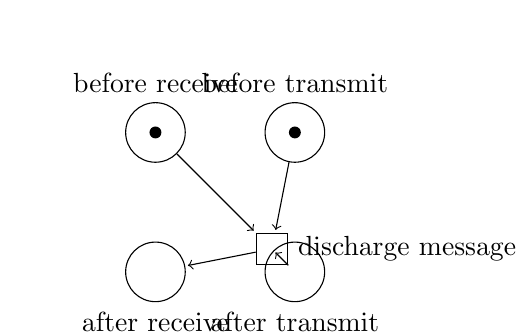
\begin{tikzpicture}
  \node[place,tokens=1,label=above:{before receive}] (beforeRx) {};
  \node[place,tokens=1,right = of beforeRx, label=above:{before transmit}] (beforeTx) {};
  \node[place,tokens=0,below=of beforeRx, label=below:{after receive}] (afterRx) {};
  \node[place,tokens=0,below=of beforeTx, label=below:{after transmit}] (afterTx) {};
  \node[transition,below right=of beforeRx, label=right:{discharge message}] (trans) {}
  edge [pre] (beforeRx)
  edge [pre] (beforeTx)
  edge [post] (afterRx)
  edge [post] (afterTx);
\end{tikzpicture}

Discharging a message here means copying the relevant bits of state from the transmitting thread's local state into the receiving thread's local state.
A message can be discharged if there is one thread willing to send it and one thread willing to receive it.
While the message is being discharged the two threads are effectively merged, with only one thread actually executing the message side effects.
Once the message is finished the two threads separate again and continue to execute independently.

A thread is only willing to receive a message if the message would pass the thread's message filter.
This has two parts:

\begin{itemize}
\item
  The message must have the correct message ID.
  This simply means that the send and receive parts of the message operation must be trying to enforce the same happens-before edge.
\item
  The message must pass the receiving thread's message receive filter.
  This filter consists of all of the side-conditions present in the crash enforcement plan which will become evaluatable once the message has been received.
\end{itemize}

However, in a real implementation, the threads are not pre-specified, and most of the complexity of the message algorithm lies in determining them.
When the plan demands that a message be sent or received, one side can be determined trivially, but the other must be discovered.
For a receive operation, the algorithm to do so in the abstract semantics looks like so:

\begin{algorithmic}[1]
  \IF {$l$ has a bound thread}
    \IF {The bound thread does not have an outgoing message}
      \STATE {Wait for it to send one}
    \ENDIF
    \IF {The bound thread has an outgoing message and it passes the message filter}
      \STATE {Discharge the message}
    \ELSE
      \STATE {$l$ has failed; remove it from the active set}
    \ENDIF
  \ELSE
    \STATE {Examine the set of outstanding unbound message sends and collect all of the ones which pass the message filter into $s$}
    \STATE {Extend $s$ with $\bot$}
    \STATE {Choose $s'$ non-deterministically from $s$}
    \IF {$s\prime = \bot$}
      \STATE {Register $l$ as a receiver of unbound messages}
      \STATE {Wait for the delay specified in this receive operation}
      \STATE {Unregister $l$ as a receiver of unbound messages}
      \STATE {Collect all of the unbound sends which pass the filter which started while we were waiting into $s$}
      \STATE {Select $s'$ non-deterministically from $s$}
    \ENDIF
    \STATE {Discharge $s'$}
  \ENDIF
\end{algorithmic}

The send operation is symmetric:

\begin{algorithmic}[1]
  \IF {$l$ has a bound thread}
    \IF {The bound thread is attempting to receive a message}
      \STATE {Wait for it to start receiving}
    \ENDIF
    \IF {The bound thread is receiving a message and this message would pass its filter}
      \STATE {Discharge the message}
    \ELSE
      \STATE {$l$ has failed; remove it from the active set}
    \ENDIF
  \ELSE
    \STATE {Examine the set of outstanding unbound message receives and collect all of the ones whose filters this message would pass into $s$}
    \STATE {Extend $s$ with $\bot$}
    \STATE {Choose $s'$ non-deterministically from $s$}
    \IF {$s' = \bot$}
      \STATE {Register $l$ as a sender of unbound messages}
      \STATE {Wait for the delay specified in this receive operation}
      \STATE {Unregister $l$ as a sender of unbound messages}
      \STATE {Collect all of the unbound receives whose filters this message would pass which started while we were waiting into $s$}
      \STATE {Select $s'$ non-deterministically from $s$}
    \ENDIF
    \STATE {Discharge $s'$}
  \ENDIF
\end{algorithmic}

As shown in figure ..., each message operation effectively defines an interval in time, and a send and receive match up if these windows overlap.
The behaviour when $s' = \bot$ is perhaps somewhat surprising: the thread waits a little while and then selects a peer thread to discharge the message with non-deterministically.
Meanwhile, all of the other threads are simultaneously performing similar non-deterministic choices.
The use of look-ahead nondeterminism means that all of the threads will make these selections in a mutually compatible way, so that there is no danger of A attempting to discharge its message with B while B discharges with C.
The actual implementation must resolve these constraints much more carefully, and is discussed in detail later.

Note that the message receive filter is evaluated as the message is being discharged, while the two threads are merged.
It is possible to imagine an alternative implementation in which the filter is instead evaluated locally in the receiver after the discharge operation is complete.
This would reduce the size of the synchronised section and so would appear, on the face of it, to offer greater parallelism, and hence potentially better performance.
Unfortunately, it does not work.
To illustrate the problem, consider again the example shown in figure \todo{...}.
One thread modifies a shared structure while another thread reads it, and the program will crash if the two threads happen to be operating on the same structure at the same time.
Suppose that the read thread runs far more often than the write one and that there are many instances of the structure.
The timeout balancing logic will quickly reduce the delay on the read side's first message send to zero and increase the delay on the write side's first message receive to compensate.
Now, when the write thread does run, it will stop just before \verb|l9| waiting for a matching read thread to arrive.
By hypothesis, many such threads will arrive, as the read thread runs more often than the write one.
In the alternative design, the read thread cannot evaluate the write thread's receive filter, and so every read thread will attempt to bind to the write thread, forcing the write thread to be duplicated many times.
Because of timeout rebalancing, the read thread will proceed from \verb|l2| immediately and quickly reach \verb|l5|, where it has to receive a message from \verb|l9|.
At this point, there are two possible outcomes:

\begin{itemize}
\item
  The thread is delayed at \verb|l5| waiting for the message from \verb|l9|.
  The write thread is still waiting in case any other threads reach \verb|l2| and attempt to synchronise with it, and so this might potentially be a rather long delay.
  Since the read thread runs far more often than the write thread, this will have a very large performance impact.
  Worse, it will probably be pointless: there, by hypothesis, a large number of instances of the structure which is being examined, and so, with high probability, the write thread will be modifying a different one.
  When the write thread does finally escape from its receive delay and evaluate its receive filter it will discover that the filter fails, and so the write thread will exit.
  The read thread will then discover that its bound thread has exited and be forced to exit as well.
  The crash enforcement plan will therefore not complete and the bug is highly unlikely to reproduce.
  
  Even worse, the performance hit might mean that the read thread will run far less frequently, further reducing the likelihood of the bug reproducing.
  In extreme cases, the attempt at enforcing a crash might actually make the bug less likely to reproduce in unit time.
\item
  The thread is not delayed at \verb|l5|.
  It never receives the message from \verb|l9| and must therefore exit without completing the plan, so is unlikely to reproduce the bug.
  The write thread's high-level interpreter will then accumulate a collection of low-level threads which have bound to exited read threads and which will themselves immediately exit.
\end{itemize}

Neither outcome helps to reproduce the target bug.

By contrast, in the scheme used by SLI, the read thread is able to evaluate the write thread's message receive filter at \verb|l2|.
It will therefore only bind to write threads which modify the structure which it is reading.
That means that the thread can be delayed a relatively long time at \verb|l5| without fear of apocalyptic performance damage, and so the bug will reproduce relatively easily.

\subsubsection{Discuss the timeout balancing bit}

Selecting the size of the various timeouts is important for determining the likelihood of reproducing a bug and the overheads of enforcing the patch.
SLI does so primarily dynamically, in response to the program's observed behaviour.

\subsubsection{Implementing non-deterministic choice in the Succ phase}

It might be that an instruction has several possible successors in the control flow graph in the crash execution plan, and in that case the interpreter must choose one of these successors using look-ahead non-determinism.
This cannot be implemented in any physically-realisable system, as it is non-causal, and so SLI must emulate it.
SLI uses a power-set construction to do so.
Rather than operating a single interpreter context, the actual implementation maintains a set of low-level interpreter contexts, which roughly follow the abstract semantics given above, and interprets them all in lock-step parallelism.
When one of these low-level interpreters needs to perform a non-deterministic choice between $n$ possible values, the high-level interpreter creates $n$ successor low-level interpreter states, one corresponding to each possible outcome of the choice, and inserts all of them into its current-state set.
They are then interpreted in parallel until enough information is available to resolve the earlier choice, at which point all but one of the threads will exit and the interpreter can revert to single-threaded execution.
If a thread is bound when it performs a non-deterministic choice then its bound thread must also be duplicated, to ensure that the new thread has something to bind to.

One subtlety here is that the original program's underlying instruction can only be retired once, and so the high-level interpreter must ensure that all low-level interpreters arrive at that point in the execution cycle at the same time.
SLI actually enforces a slightly stronger constraint, which is that every low-level interpreter in a given high-level interpreter must be at the same phase in the instruction execution cycle.
The only phases for which this is difficult are the message send and receive phases, which are discussed in more detail in the next section.

\subsubsection{Concrete implementations of message send and receive}

The message receive operation looks like this:

\begin{algorithmic}[1]
  \STATE {$lls \gets $ the set of currently-active low-level interpreter states}
  \STATE {$newLls \gets $ an empty set of low-level interpreter states}
  \FORALL {$l$ in currently-active low-level interpreter states}
    \IF {$l$ does not receive any messages}
      \STATE {Move $l$ from $lls$ to $newLls$ without changing it}
    \ELSIF {$l$ has a bound thread}
      \IF {$l$'s bound thread has exited}
        \STATE {$l$ exits as well; remove it from $lls$ without adding it to $newLls$}
      \ELSIF {$l$'s bound thread has an outgoing message}
        \IF {The bound thread's outgoing message passes the message filter}
          \STATE {Copy stashed values from the sending low-level interpreter's state to the receiving one}
          \STATE {Move $l$ from $lls$ to $newLls$}
        \ELSE
          \STATE {$l$ exits; remove it from $lls$}
        \ENDIF
      \ELSE
        \STATE {} \COMMENT {Wait for a the bound thread to send a message}
      \ENDIF
    \ELSE
      \STATE {} \COMMENT{Unbound receive}
      \FORALL {$s$ registered unbound senders}
        \IF {$s$'s outgoing message passes the message filter}
          \STATE {$l' \gets $ duplicate $l$}
          \STATE {$s' \gets $ duplicate $s$}
          \STATE {Copy stashed values from $s'$'s state to $l'$'s}
          \STATE {Bind $l'$ and $s'$ together}
          \STATE {Insert $l'$ into $newLls$}
          \STATE {Insert $s'$ into $s$'s high-level interpreter's active low-level interpreter list}
        \ENDIF
      \ENDFOR
      \STATE {Register $l$ as an unbound receiver}
    \ENDIF
  \ENDFOR

  \IF {$lls$ is empty}
    \RETURN
  \ENDIF

  \STATE {$end \gets now() + bound\_delay$}
  \IF {There is a minimum delay}
    \STATE {Release lock}
    \STATE {Sleep for the minimum delay}
    \STATE {Acquire lock}
  \ENDIF

  \WHILE {There are bound receives in $lls$ and $now() < end$}
    \STATE {Release lock}
    \STATE {Wait for some bound receive to complete, or for the current time to pass $end$}
    \STATE {Acquire lock}
    \FORALL {$l$ performing bound receives in $lls$}
      \IF {$l$'s bound thread has exited}
        \STATE {Remove $l$ from $lls$}
        \STATE {$l$ exits}
      \ELSIF {$l$'s receiving-bound-message flag is clear}
        \STATE {Remove $l$ from $lls$}
        \STATE {Add $l$ to $newLls$}
      \ELSE
        \STATE Continue waiting
      \ENDIF
    \ENDFOR
  \ENDWHILE

  \FORALL {$l$ in $lls$}
    \IF {$l$ is registered as an unbound receiver}
      \STATE {Unregister $l$ as an unbound receiver}
    \ENDIF
    \IF {$l$ was attempting a bound receive and the bound thread hasn't sent any messages}
      \STATE {Exit $l$}
    \ELSIF {$l$ is unbound}
      \STATE {The thread must have been attempting an unbound receive which failed, so exit $l$}
    \ELSE
      \STATE {} \COMMENT {Receive succeeded}
      \STATE {Add $l$ to $newLls$}
    \ENDIF
  \ENDFOR

  \STATE {Set high-level interpreters set of currently-active low-level interpreters to $newLls$}
\end{algorithmic}

The send algorithm is very similar:

\begin{algorithmic}[1]
  \STATE {$lls \gets $ the set of currently-active low-level interpreter states}
  \STATE {$newLls \gets $ an empty set of low-level interpreter states}
  \FORALL {$s$ in currently-active low-level interpreter states}
    \IF {$s$ does not send a message}
      \STATE {Move $l$ from $lls$ to $newLls$ without changing it}
    \ELSIF {$s$ has a bound thread}
      \IF {$s$'s bound thread has exited}
        \STATE {$s$ exits as well; remove it from $lls$ without adding it to $newLls$}
      \ELSIF {$s$'s bound thread is waiting to receive a message}
        \IF {$s$'s outgoing message passes the message filter}
          \STATE {Copy stashed values from the sending low-level interpreter's state to the receiving one}
          \STATE {Move $s$ from $lls$ to $newLls$}
          \STATE {Clear the bound thread's receiving-bound-message flag}
        \ELSE
          \STATE {$s$ exits; remove it from $lls$}
        \ENDIF
      \ELSE
        \STATE {} \COMMENT {Wait for a the bound thread to be ready to receive a message}
      \ENDIF
    \ELSE
      \STATE {} \COMMENT{Unbound send}
      \FORALL {$l$ registered unbound receivers}
        \IF {The outgoing message passes $l$'s message filter}
          \STATE {$l' \gets $ duplicate $l$}
          \STATE {$s' \gets $ duplicate $s$}
          \STATE {Copy stashed values from $s'$'s state to $l'$'s}
          \STATE {Bind $l'$ and $s'$ together}
          \STATE {Insert $s'$ into $newLls$}
          \STATE {Insert $l'$ into $l$'s high-level interpreter's active low-level interpreter list}
        \ENDIF
      \ENDFOR
      \STATE {Register $s$ as an unbound sender}
    \ENDIF
  \ENDFOR

  \IF {$lls$ is empty}
    \RETURN
  \ENDIF

  \STATE {$end \gets now() + bound\_delay$}
  \IF {There is a minimum delay}
    \STATE {Release lock}
    \STATE {Sleep for the minimum delay}
    \STATE {Acquire lock}
  \ENDIF

  \WHILE {There are bound sends in $lls$ and $now() < end$}
    \STATE {Release lock}
    \STATE {Wait for some bound send to complete, or for the current time to pass $end$}
    \STATE {Acquire lock}
    \FORALL {$s$ performing bound sends in $lls$}
      \IF {$s$'s bound thread has exited}
        \STATE {Remove $s$ from $lls$}
        \STATE {$s$ exits}
      \ELSIF {$s$'s sending-bound-message flag is clear}
        \STATE {Remove $s$ from $lls$}
        \STATE {Add $s$ to $newLls$}
      \ELSE
        \STATE Continue waiting
      \ENDIF
    \ENDFOR
  \ENDWHILE

  \FORALL {$s$ in $lls$}
    \IF {$s$ is registered as an unbound sender}
      \STATE {Unregister $s$ as an unbound sender}
    \ENDIF
    \IF {$s$ was attempting a bound send and the bound thread hasn't tried to receive any messages}
      \STATE {Exit $s$}
    \ELSIF {$s$ is unbound}
      \STATE {The thread must have been attempting an unbound send which failed, so exit $s$}
    \ELSE
      \STATE {} \COMMENT {Send succeeded}
      \STATE {Add $s$ to $newLls$}
    \ENDIF
  \ENDFOR

  \STATE {Set high-level interpreters set of currently-active low-level interpreters to $newLls$}
\end{algorithmic}

One further optimisation, not shown here, avoids redundantly duplicating low-level interpreter contexts in the common case that a message operation is discharged precisely once.

\todo{This is probably not the best way of presenting those
  algorithms.}

\todo{Discuss setting minimum delays here}

\subsubsection{The await-bound-thread-exit state}

When a thread completes its plan, it is sometimes useful for it to wait for its bound thread to exit before proceeding.
This is because the crash summary from which the plan is generated does not have complete information on the structure of the program.
If the last edge in a happens-before graph is from memory access A to memory access B, that generally means that A is a store and B is a load and B must load the value stored by A.
That means that, not only must B happen after A, but B must happen before any other writes to the memory location modified by A.
If there were other stores to that location in the crash summary then the happens-before graph would include additional edges to ensure that that happens, but if there are stores outside of the summary then it will not.
For instance, suppose that the write thread looks like this:

\begin{verbatim}
while (1) {
l1:  *x = 5;
l2:  *x = 7;
     <something_complicated>
}
\end{verbatim}

And the read thread looks like this:

\begin{verbatim}
l3: a = *x;
l4: b = *x;
    crash if a != b;
\end{verbatim}

This program is clearly buggy.
One way of reproducing this bug would be to interleave instructions as \verb|l1|, \verb|l3|, \verb|l2|, \verb|l4|.
SLI will discover this interleaving as the happens-before graph show in figure \todo{...}.
The algorithm described so far will be sufficient to enforce this graph (assuming that the two fragments of code shown can actually execute in parallel).
This is not, however, sufficient to cause the program to crash, because the generated happens-before graph is incomplete: it misses the edge from \verb|l4| to \verb|l1| in the next iteration of the loop.
If the loop completes and reaches the store at \verb|l1| before the load \verb|l4| completes then the bug will not reproduce even though the happens-before graph was successfully enforced.
Any scheme with an analysis horizon based on a simple instruction count will suffer from a similar problem, but this is particularly serious for SLI, because the delays inserted are in almost precisely the right place to maximise the chance of this kind of bug-hiding race.
Returning to the example, SLI's crash enforcement plan will include a delay after \verb|l1| (to implement the \verb|l1| to \verb|l3| happens-before edge), and this delay will be large relative to a short sequence of normal instructions, and so the bug will be hidden completely provided that the delay to wake up the read thread after the final edge is greater than the time taken to execute \verb|<something_complicated>|.
This is perfectly plausible, given that \verb|<something_complicated>| only needs to be a few dozen instructions to exceed SLI's analysis window.
This bug will therefore never reproduce under SLI's crash enforcer, even when the happens-before graph is enforced perfectly.
The fix is simple: have the store thread delay slightly after completing its final message send operation, until the read thread also completes its crash enforcement plan.
This ensures that activity beyond the analysis horizon cannot prevent bug reproduction, and, because it only happens when the plan is mostly complete, and hence happens very rarely, it has very low performance overhead.

\begin{tikzpicture}
\node[CfgInstr] (l1) {l1};
\node[CfgInstr, below = of l1] (l2) {l2};
\node[CfgInstr, right = of l1] (l3) {l3};
\node[CfgInstr, below = of l3] (l4) {l4};
\draw[->] (l1) -- (l2);
\draw[->] (l3) -- (l4);
\draw[->,happensBeforeEdge] (l1) -- (l3);
\draw[->,happensBeforeEdge] (l3) -- (l2);
\draw[->,happensBeforeEdge] (l2) -- (l4);
\end{tikzpicture}


\subsubsection{Compiling the plan}

\todo{Implementation of this is currently massively broken; need to
  decide whether I'm going to fix it or just use a slightly older
  version.}

In addition to a plan interpreter, SLI also includes a plan compiler, which combines the plan with the program's original machine code to produce a modified version of the program which performs the necessary enforcement actions without needing an interpreter.
The intent here is to reduce the overhead of the interpreter in the case where SLI is investigating many bugs most of which do not exist.
Making this practical requires several simplifications to the semantics:

\begin{itemize}
\item
  The number of physical program threads operating in the plan is limited.
  In particular, it is assumed that only one program thread will be executing the read side of the plan at any time, and likewise only one thread will be executing the write side.
\item
  The message semantics are simplified: messages are sent asynchronously, with a delay only on the read side, and must be ``cancelled'' when the relevant thread exits.
  This has two important implications: first, that a message send can never fail and, second, the something must keep track of what messages a given thread currently has outstanding.
  Combined with the first simplification, it also means that at most one instance of any given message can be outstanding at any one time, and so it is easy to place the relevant information in a global structure without needing any dynamic memory allocation.
\item
  High-level interpreter contexts only ever access the state of their own low-level interpreters.
  This has two important implications:

  \begin{itemize}
  \item
    Remote low-level interpreters are never duplicated during message operations.
    If the normal semantics would require an interpreter to be duplicated then the local message operation fails.
  \item
    The receive message filter can only be executed by the receiving thread after receiving a message.
  \end{itemize}
\item
  When a low-level interpreter is duplicated due to a non-deterministic choice in the Succ phase the low-level state's stash table is not duplicated.
  Instead, all low-level interpreters in a given high-level interpreter share a single stash table.
\end{itemize}

The result is a system with lower run-time overheads, but also a lower probability of reproducing interesting bugs.
It has a much larger I-cache footprint but a smaller D-cache one\editorial{Not sure where I'm going with that, although it is true and kind of interesting}.

I now briefly outline the implementation of this compiler.
The core idea is to compile the CFG in the enforcement plan into a state machine.
This state machine consists of a large number of smaller intra-instruction state machines, as illustrated in figure~\todo{...}, each of which models a single instruction in the original program.
The label on each state is itself a set of low-level labels which consist of a four-tuple of the plan thread which is executing, a reference to the plan CFG node, a set of messages which have been sent by the thread, and the phase of the intra-instruction state machine.
Each state is compiled to a small fragment of machine code (which might be empty, if this instruction does not have an relevant annotation in the plan) plus a set of relocations specifying the fragment's relationships to the other states.
Once every state has been compiled these relocations can be discharged and the fragments concatenated together to form the final patch.

I now discuss the details of each phase of the intra-instruction machine:

\begin{itemize}
\item[RecvMsg]
  Examine the set of CFG nodes which are active in the current state and determine whether the plan requires any of them to receive messages.
  If so, emit code to examine the global outstanding-message structures to see whether of the desired messages are currently outstanding.
  If there are, receive precisely that message.
  Any other message receive operations are considered to have failed and the relevant CFG nodes removed from the current state label.
  If no message sends are currently outstanding then the physical thread is delayed until either one is available or some timeout is reached.
  If a message becomes available then it is received, and otherwise all receives fail and all receiving CFG nodes are removed from the label.
  Note that this does not necessarily mean that the state label will become empty\footnote{Although that is the common case.} as there may be some CFG nodes which do not need to receive messages.

  Once a message is received its content is simply copied from the global message area into the local thread's stash area.
\item[OrigInstr]
  Store any generated values into simulation slots and issue the original instruction.
  There are three main cases to consider here:

  \begin{itemize}
  \item
    Simple memory loads.
    If the instruction is of the form \verb|LOAD *location -> register|, and the value loaded is to be saved, then it is sufficient to just copy \verb|register| into the simulation slot after the original instruction has completed.
  \item
    Compound memory loads.
    Instructions which load from memory but are not themselves simple loads are more difficult to handle.
    For concreteness, suppose that the instruction is \verb|CMP 76,*loc1|, and the annotation requires us to save the value loaded.
    The instruction loads from \verb|*loc1| but does not leave the result in any locations which we can easily access.
    It would be possible to solve this problem by adding another load of \verb|*loc1|, but that would run the risk of a store in a remote thread modifying \verb|*loc1| between the two loads, leading to very confusing results.
    SLI instead solves this problem by rewriting the instruction to this:

\begin{verbatim}
LOAD *loc1 -> reg1
STORE reg1 -> simslot
CMP 76, reg1
\end{verbatim}

    This exposes the loaded value to the instrumentation framework, allowing it to be stored to the simulation slot as desired.

    Instructions which modify memory in-place, such as \verb|ADD 1 + *loc1 -> *loc1|, pose a similar problem and can be solved in the same way, provided that they do not have a \verb|LOCK| prefix.
    \verb|LOCK|ed instructions are more complex, as separating the load and store phases into separate instructions would violate the semantics of the program and might introduce new bugs.
    SLI solves this problem using a \verb|CMPXCHG| loop.
    For instance, the instruction \verb|LOCK ADD 1 + *loc1 -> *loc1| would be converted to this machine code fragment:

\begin{verbatim}
1: LOAD *loc1 -> reg1
ADD 1 + reg1 -> reg2
LOCK CMPXCHG *loc1, reg1 -> reg2
if_cmpxchg_failed goto l1
STORE reg1 -> simslot
\end{verbatim}

    The \verb|CMPXCHG| instruction here is supposed to be an invented syntax for the x86 machine code instruction which atomically compares \verb|*loc1| to \verb|reg1| and, if they are equal, sets \verb|*loc1| to \verb|reg2|.
    This allows SLI to expose the value of the implicit load while preserving the \verb|LOCK| semantics of the original instruction.
  \item
    Branch instructions are deferred to the FindSucc state.
  \end{itemize}
  
\item[SendMsg]
  Send any outgoing messages.
  This amounts to simply copying the message payload into the global message area, setting a global flag to indicate that the message is currently outstanding, and adding the message ID to the state label's set of sent messages.
  This always succeeds and advances to the FindSucc state.

\item[ExitThread]
  When a low-level thread exits it is necessary to cancel any messages which it has sent.
  The compiler takes the union of all of the sent-messages sets in its low-level, removes the thread which is to exit, and then takes the union again.
  Any messages present in the first set but not the second need to be cancelled by setting the relevant global message-outstanding flag to zero.
  The compiler will then either exit the patch, if the last low-level thread has exited, or resume the intra-instruction state machine at an appropriate place.
\end{itemize}


\begin{tikzpicture}
\node[flowChartState] (RecvMsg) {RecvMsg};
\node[flowChartState,above left = of RecvMsg] (StartThread) {StartThread};
\node[flowChartState,above right = of RecvMsg] (CheckForThreadStart) {CheckForThreadStart};
\node[flowChartState, below = of RecvMsg] (OrigInstr) {OrigInstr};
\node[flowChartState, below = of OrigInstr] (VerfCond) {VerfCond};
\node[flowChartState, below = of VerfCond] (SendMsg) {SendMsg};
\node[flowChartState, below = of SendMsg] (FindSucc) {FindSucc};
\node[flowChartState, right = of VerfCond] (CondFail) {CondFail};
\node[flowChartState, right = of CondFail] (Exit) {Exit};
\node[flowChartState, left = of RecvMsg] (RecvdMsg) {RecvdMsg};
\draw[->] (CheckForThreadStart) -- (RecvMsg) -- (OrigInstr) -- (VerfCond) -- (SendMsg) -- (FindSucc);
\draw[->] (StartThread) to [bend right=10] (CheckForThreadStart);
\draw[->] (CheckForThreadStart) to [bend right=10] (StartThread);
\draw[->,dashed] (FindSucc.east) to [bend right=75] (CheckForThreadStart.east);
\draw[->] (RecvMsg) -- (RecvdMsg) -- (OrigInstr);
\draw[->] (RecvMsg) -- (Exit);
\draw[->] (VerfCond) -- (CondFail) -- (Exit);
\draw[->] (FindSucc) -- (Exit);
\end{tikzpicture}

  

\subsubsection{Compiling entry point stubs}
\label{sect:find_bugs:compile_entry_points}

\todo{Good Lord, this is completely incomprehensible.}

The entry points of the crash enforcement plan are given as mappings from call stacks to CFG nodes.
The program must be patched so that it transfers control to the interpreter whenever the call stack matches up with one of these entry-point call stacks.
This is a multi-step process:

\begin{itemize}
\item
  The last pointer in the call stack is a raw instruction pointer.
  The relevant instruction is patched into a jump into the interpreter trampoline.
\item
  The interpreter trampoline transitions to a different stack, saves the client program's register state, and starts the main interpreter.
\item
  The main interpreter then examines the program's stack to determine whether it matches up with the entry-point stack.
  If it does then a new high-level interpreter state is created and interpretation starts.
  Otherwise, the interpreter exits back to the original program (possibly after emulating enough instructions to avoid returning into the middle of the new jump instruction).
\end{itemize}

The last point is more subtle than it might appear, as the interpreter must be able to find arbitrary return addresses on the program's stack, and this is difficult if the program is compiled without frame pointers or debug symbols.
SLI uses a static analysis, performed when generating the crash enforcement plan, to solve this problem.
The static analyses already described are sufficient to determine the entry point of the function containing a given RIP, and so it is easy to perform a simple abstract interpretation forwards from that point to the given RIP and hence find the number of bytes which the function will push onto the stack on the way\footnote{This is generally fixed for all possible paths}.
The first entry in the call stack is trivially true because of the way the jumps are patched in.
The second one is the return address of the current function, which can be found using that offset.
The third one is the return address of the calling function, and the offset there is just the previous offset plus the offset in the calling function.
In this way all necessary offsets can be found and the entry-point stack checked completely.

\subsubsection{Run-time considerations}

Recovery from spurious segfaults in the patch due to e.g. LD operations.

\subsection{Comparison to schedule memoisation}
\subsection{Comparison to STM block inference stuff}



\chapter{Other modes of operation}
\section{Fixing bugs}

\subsection{Using global locks}
\label{sect:fix_global_lock}

\todo{Write me.  This is supposed to be about how you patch in lock-acquire and lock-release operations.}

\subsection{Using a message-passing network}
\todo{I've come up with an algorithm for doing this, but I really don't have time to implement it.  It is kind of cool, though; I'd like to include it somewhere, even if it's just a future work-type thing.}

\section{Fixing bugs from DRS logs}
The simplest way to fix a bug is to start from a DRS log.
Given a log, identifying the thread and which is most responsible for a crash is generally straightforward.
If the crash is caused by dereferencing a bad pointer then the responsible thread is the one which dereferenced the pointer; if the crash is an assertion failure then the responsible thread is the one which called \verb|abort()| (or equivalent).
The log then makes it trivial to determine what instructions the responsible thread executed before it crashed, and a suffix of these can be compiled into a \StateMachine capturing the most relevant parts of the responsible thread's behaviour.

The log also makes it trivial to determine precisely which stores the read-side thread raced with, and so building a write-side \StateMachine is redundant.
Instead, the read-side \StateMachine is ``slid across'' the log, evaluating it at every step (subject to some typing constraints which ensure that the result is reasonable), and the resulting pattern of safe and unsafe regions converted directly into critical sections, without ever needing to generate an explicit write-side \StateMachines.

\subsection{Building the read-side \StateMachine}
\todo{This is gratuitously different from the non-DRS mode in an enormous number of places.  I should fix that.}

Working from a DRS log provides a lot of information which is not available in SLI's normal mode of operation.
This makes some parts of the algorithm redundant.
In particular, there is no need to generate large numbers of CFGs of fragments of the program which might be relevant, as we know precisely which instructions were executed leading up to the crash.
Instead, in this mode, SLI generates the \StateMachine directly from the log.
It starts with a small stub machine representing just the instruction which crashed and then expands it backwards, incorporating a single instruction from the log at a time.
For instance, suppose that the fragment of program to be investigated looked like this:

\begin{verbatim}
l1: mov $5, %rax
l2: mov (global1), %rbx
l3: mov (%rax + %rbx), %rcx
\end{verbatim}

and the program crashed due to dereferencing a bad pointer at \verb|l3|.
The initial stub \StateMachine will then be just:

\begin{verbatim}
if (BadPtr(rax + rbx)) crash(); else survive();
\end{verbatim}

Incorporating \verb|l2| will transform that to

\begin{verbatim}
LOAD (global1) -> rbx
if (BadPtr(rax + rbx)) crash(); else survive();
\end{verbatim}

Incorporating \verb|l1| will then produce the \StateMachine

\begin{verbatim}
COPY 5 -> rax
LOAD (global1) -> rbx
if (BadPtr(rax + rbx)) crash(); else survive();
\end{verbatim}

Which can be simplified in the usual way to produce

\begin{verbatim}
LOAD (global1) -> rbx
if (BadPtr(rbx)) crash(); else survive();
\end{verbatim}

And this can then be used in the rest of the analysis.

The major subtlety here lies in the handling of control flow, and the parts of the program which are not executed.
One possible approach would be to simply say that any changes to the control flow cause the bug to be avoided, but this is over-optimistic.
Consider, for instance, a program like this one:

\begin{verbatim}
ptr = global;
if (some_condition)
    idx = 1;
else
    idx = 2;
local = ptr[idx];
\end{verbatim}

This program loads a pointer to an array from a global variable and then loads some index in the array, with the index chosen depending on some condition.
Suppose that the race then causes the pointer in \verb|global1| to sometimes be bad, and that the reproduction of the bug was obtained while \verb|some_condition| holds.
The bug itself does not depend on \verb|some_condition|, but if one were to assume that any changes to control flow avoid the bug then SLI would not be able to show this.
This problem can only be avoided by exploring untaken branches, and SLI does so, for some (configurable) number of instructions.
If the control flow rejoins that which is represented in the DRS log then an appropriate branch is included from one part of the \StateMachine to another, and if it does not rejoin then a branch to the \verb|NoCrash| state is used instead.

One complication here is that a given static instruction might be represented multiple times in the DRS instruction trace, and hence multiple times in the \StateMachine, if the instruction is part of some loop.
This makes it ambiguous where the branch should branch to.
SLI solves this problem by taking the earliest instance of the instruction, and hence branching to the place in the \StateMachine nearest the root.
This helps to keep the loop structure of the program intact, subject to the unrolling implicit in the DRS log.

The example shown above might then turn into a \StateMachine something like this:

\begin{verbatim}
LOAD global1 -> ptr
if (some_condition) {
   COPY 1 -> idx1
} else {
   COPY 2 -> idx2
}
if (BadPtr(ptr + idx)) {
   crash();
} else {
   survive();
}
\end{verbatim}

The standard simplified will then transform that to this:

\begin{verbatim}
LOAD global1 -> ptr
if (BadPtr(ptr + (some_condition ? 1 : 2))) {
   crash();
} else {
   survive();
}
\end{verbatim}

SLI uses a rule that \verb|BadPtr(x + k)| is equivalent to \verb|BadPtr(x)| whenever \verb|k| is a small constant, and so correctly determines that the bug is independent of \verb|some_condition| in this case.

\todo{Discuss using more powerful bug definitions here e.g. Valgrind, invariant discovery, etc, by applying them to the log and then converting to stub machines, so that you can apply this to races which lead to bugs other than immediate bad pointer dereferences.}

\subsection{Requirements on the DRS}

\subsection{Finding remote critical regions}

The fixes generated by SLI rely on making the read-side \StateMachine operate as-if atomically and then ensuring that it does not execute in any states where doing so would lead to a crash.
In the normal mode of operation, the regions which would lead to a crash are determined by modelling the rest of the program as a set if write-side \StateMachines and then using symbolic execution, but it is possible to be more accurate\editorial{or possibly precise?} if a full DRS log is available.
Instead of the set of \StateMachines, the log itself can be used as a model for the rest of the program.
The idea here is that the log contains a sequence of possible states of the program, and contains all of the ones which are relevant to this particular way of reproducing the bug of interest.
SLI therefore slides the read-side \StateMachine over this log, evaluating it at every instruction, and hence classifies the log into ``safe'' and ``unsafe'' regions, and the transitions between these two types of region give the boundaries of the write-side critical regions.

As a minor optimisation, SLI only re-evaluates the \StateMachine if there has been a store to some memory location which is loaded by the \StateMachine.
This cannot affect the results in any way, but means that the \StateMachine does not have to be evaluated as often.

One important complication here is the presence of dynamically-allocated data structures.
SLI relies on being able to identify points in the program where these are allocated and released.
The loads in the read \StateMachine will correspond to specific load operations in the DRS log and SLI is then able to check which dynamic instance of structures those accesses access and will only evaluate the \StateMachine while all of the relevant structures remain live.

Once the log has been classified, the classification must be converted into realisable critical sections.
In other words, SLI must identify points in the program at which it must insert lock acquire operations and points where it must insert lock release operations.
Ideally, each unsafe region in the log would correspond to a single critical section, with a single acquire operation and a single release one.
This can fail in several ways:

\begin{itemize}
\item
  The start and end of the unsafe region might be in different threads, if, for instance, one thread violates an invariant and another thread then restores it.
  It is difficult to model a cross-thread operation as a critical section.
  SLI cannot prevent this kind of bug, and the unsafe region is simply ignored.
\item
  There might be non-trivial control flow between the start and end of an unsafe region within a single thread.
  In that case additional acquire and release operations must be inserted to ensure that locks are not leaked, double-acquired, or double-released.
\item
  The program might have additional synchronisation mechanisms which, when combined with the SLI-inferred synchronisation, lead to a deadlock.
\end{itemize}

These are discussed in more detail in \S~\ref{sect:fix_global_lock}.

\todo{This is in dire need of rewriting.}

Note that the definition of a dynamic structure is somewhat subtle here.
Most obviously, \verb|malloc| and \verb|free| represent boundaries in the lifespan of such structures (with \verb|malloc| being the start and \verb|free| being the end), but ``re-typing'' operations can also impose such boundaries.
The intent of the sliding procedure is to capture other operations which the program might perform on the data structures involved in the synchronisation bug, in the same way that write-side \StateMachines do in the non-DRS case.
In effect, the program's behaviour is constrained using a heuristic memory safety property, and this memory safety property must correspond reasonably closely to the program's actual structure.

The underlying hypothesis here is that the program has some kind of internal type system which constrains which operations will be performed on a given memory location.
This means that two pieces of code can only race if they have types which are in some sense compatible, so that they might access overlapping memory locations.
The combination of the read-side \StateMachine and the set of dynamic instances accessed by it defines, in a slightly ill-defined way, a set of types which the read side of the critical section might access.
SLI must then find some other operations on the same types to synchronise against, and this is the aim of the sliding procedure.
In order for this to work, the read \StateMachine must only be slid to places where the current types match up with the types for which it was derived.
SLI must therefore be able to identify points where the types of memory locations change.
This includes things like \verb|malloc| and \verb|free|, but is also likely to include things like program-specific memory allocators or object pools.
The precise set will depend on the program's type system, and so can only be sensibly modelled with assistance from the programmer.




\chapter{Analysis on \StateMachines}
Things which are worth discussing here:

\begin{itemize}
\item
  Give a very brief discussion of the actual analysis passes I use.
  Most of these will just be refs to the standard program slicing/decompilation/compilers literature.
  Deadcode and avail belong here.
\item
  Explicit discussion of the undefinedness analysis, because the argument which shows it to be sound is really rather subtle, and I've not seen anyone else make it.
\item
  Probably mention that we sometimes optimise on the assumption that assertion failures correspond to crashes and sometimes on the assumption that correspond to avoiding the crash, and discuss why that's necessary.
\item
  Maybe discuss getting rid of local survival constraints?
\item
  The function alias analysis and phi elimination analyses are kind of interesting; I haven't seen them anywhere else (and they're inherently cross-function, rather than the usual compilers approach of just inlining everything and then doing intra-function analysis on that, which is kind of fun).
\item
  The encoding of multiple fragments of program into a single \StateMachine, which reduces analysis costs quite a bit, is kind of interesting.
\item
  The encoding of the static analysis information into the \StateMachines, to expand the context sensitivity horizon, is also kind of interesting.
\end{itemize}

\section{Alias analysis}

SLI's \StateMachines represent a cross-function slice of the program's
machine code, including a large number of memory-accessing
instructions.  This presents a non-trivial alias analysis problem.
SLI uses several techniques to resolve the resulting aliasing queries:

\begin{itemize}
\item
  First, a dynamic analysis is used to build up a model of how the
  program behaves during normal operation.  This model is generally
  reasonably effective at determining whether instructions which
  access the heap or global data might conflict, but does not contain
  information on accesses to the local stack.
\item
  Next, a static analysis pass is used to determine which instructions
  might access local variables in the current stack frame.  This
  analysis is almost entirely function-local and is applied to every
  function in the program before the main analysis pass starts.
\item
  The results of this static analysis pass are incorporated into the
  \StateMachines in a way which automatically extends them to
  accurately reflect cross-function properties of the program.
\item
  The main alias analysis can then be run on the \StateMachines
  themselves, in conjunction with the other \StateMachine
  simplification passes, to resolve aliasing queries.
\end{itemize}

I now describe each of these phases in more detail.

\subsection{Dynamic analysis}

SLI relies on a dynamic analysis pass to build up a model of the
program's behaviour when it is running normally.  This model mostly
focuses on the possible aliasing relationships between memory accesses
outside of the program's stack; in other words, determining whether
two instructions might access the same piece of non-stack memory.
This is a full alias analysis, rather than a points-to analysis, and
so could in principle need to build up a full $O(n^2)$ table showing,
for each pair of instructions whether those instructions might alias.
Fortunately, that table is rather sparse for most programs, allowing
some significant simplifications to be made.

The intuition behind this analysis is that most fields in most data
structures are accessed by a relatively small number of places in the
program, and so if it were possible to identify the field being
accessed by a given instruction then that would make it easy to
determine whether two instructions might interfere.  Unfortunately,
that kind of higher-level information is not usually available when
analysing binary programs.  SLI sidesteps that problem by identifying
fields by the set of instructions which might access them and then
assuming that instructions might alias precisely when they are part of
the same field.  The result is an alias table which can be collected
in reasonable time using a simple dynamic analysis, which can resolve
aliasing queries quickly, and which requires a tolerable amount of
space (tens of megabytes for mysqld, for instance).

Collecting the aliasing table works like this.  Memory is divided
eight byte chunks, each of which has two set of accessing instructions
associated with it, one for read instructions and one for write.  Any
instruction which accesses that memory chunk adds itself to the
relevant set.  These sets in effect identify the structure field for
the memory chunk.  When the memory dies, due to the program either
exiting or calling some \verb|free|-like function, the relevant field
descriptors are transferred to a global set of fields.  This global
set then provides the final aliasing table.

\todo{Other bits: skip stack accesses, and try to identify
  thread-private memory.}

\subsection{Static analysis}

\todo{On the one hand, this is quite important.  On the other hand,
  it's incredibly tedious.  Not sure what to do about that.}

The most important whole-program analysis used by SLI is a simple
points-to analysis which determines, for any given combination of
register and instruction, whether that register at that instruction
might point into the current stack frame (defined below) or into other
memory.  This information is then used to improve the accuracy of the
\StateMachine-level aliasing analyses.  Determining whether a memory
access is to the current stack frame is important because, in most
programs, there are a lot of them, and is relatively easy, because,
again in most programs, there are relatively few pointers into the
stack frame.  This makes the problem a reasonable choice for solving
by whole-program static analysis.

The analysis used by SLI makes several important assumptions about the
program to be analysed:

\begin{itemize}
\item
  Most importantly, it assumes that the locations in a function's
  frame are ``created'' when the function is called, in the sense that
  any pointers into the stack frame which are actually dereferenced
  must have been created after the function started.  This does not
  mean that there cannot be any pointers into the frame at the start
  of the function; simply that, if there are any, they cannot be
  dereferenced.  Pointers in dead registers are acceptable, for
  instance, as are values which are ``semantically'' integers but
  happen to have the same numerical values as valid pointers.

\item
  The analysis assumes that the location of the stack was unknown when
  the program was compiled, and in particular that any statically
  constant values are not stack pointers.  This is in some sense a
  special case of the previous assumption, but is both important and
  non-obvious and so bears additional emphasis.

\item
  The analysis assumes that all functions take all of their arguments
  in registers, and that SLI can identify the set of registers which
  might be arguments.  In the case of AMD64 using a normal ABI this is
  true for the first six arguments to a function \needRef{}, and,
  since the vast majority of functions have fewer than six arguments
  \needRef{}, this is not usually a problem.

\item
  The analysis assumes that functions will either not return at all or
  will return to the instruction following the instruction from which
  it was called.  Note that this does not rule out functions such as
  \verb|setjmp| and \verb|longjmp|: \verb|longjmp| never returns and
  \verb|setjmp| always returns to the instruction after the one which
  called it.

\item
  The analysis assumes that the stack pointer at the end of a function
  is always the same as the stack pointer at the start of that
  function, if the function returns to the same place as it was called
  from.
\end{itemize}

Given those assumptions, the first stage of the analysis is to
identify functions in the program.  For the purposes of this analysis,
a function is defined to be a (possibly non-contiguous) set of
instructions with a distinguished element, referred to as the head of
the function, such that:

\begin{itemize}
\item
  For any non-return and non-call type branch from instruction $a$ to
  $b$ anywhere in the program, either $a$ and $b$ are in the same
  function or $b$ is the head of some function, and
\item
  for any call-type branch instruction from $a$ to $b$ $b$ is the head
  of a function.
\end{itemize}

The term ``branch'' here includes the implicit branch
from one ordinary instruction to the one which immediately follows it.
Within those constraints, SLI attempts to minimise the number of
distinct functions\footnote{Or, equivalently, it maximises the size of
  the individual functions.}\editorial{Well, ``attempts to''.  There's
  no guarantee that the set is actually minimal, but it usually is.}.

For most functions, invoked using call-type branches, this definition
is straightforward, and is equivalent to saying the first instruction
in the function is the head and the function contains all instructions
reachable from that instruction until the first return-type branch,
excluding called functions.  Tail-call elimination complicates things
slightly, though.  If a function is ever called in the usual way
(i.e. not via tail-call elimination) then the first rule will cause
its first instruction to be a function head, as desired.  If a
function is never called via a call-type branch, but is tail-call
eliminated into multiple calling functions, then the second rule will
cause the join of the two calling functions' CFGs to be a function
head, and this is generally correct for simple tail-call elimination.
If the called function is only called from one place, and that place
is a tail-call, then this definition will lead to the two functions
being merged, which will lead the analysis to produce an
overly-conservative solution but will not cause an actual error.

The only slight complexity involved in discovering functions within
this definition is the handling of indirect call and branch
instructions.  SLI solves this using information from the dynamic
analysis phase: it assumes that all of the possible targets of every
indirect branch are recorded in the dynamic information, which makes
the problem trivial.

The analysis itself is then structured as a simple iteration to a
fixed point.  The iteration's state is a table saying, for each
instruction, the estimated points-to configuration at the start of the
instruction and at the end.  The end-of-instruction configuration is a
simple function of the start-of-instruction configuration and the
instruction itself, and the start-of-instruction configuration is
itself simply the union of the end-of-instruction configurations for
all of the instructions which might possibly execute immediately
before the one being analysed.  Once those rules are satisfied by each
instruction in isolation the analysis is complete and the table
provides accurate information about the program's behaviour (provided
that the assumptions given above are true).

I now give a little more detail of the various steps.

\begin{itemize}
\item
  The initial state reflects the assumptions given above.  At the
  start of the analysis, most instructions are assigned a special
  ``unreachable'' state, which says nothing at all about their
  possible points-to state.  The exceptions are function-head
  instructions, which are given this initial state:

  \begin{itemize}
  \item The stack pointer points at the current stack frame.
  \item Other registers contain either non-pointer values or pointers
    to memory outside of the current frame.
  \item There are no pointers in the current stack frame which point
    back at the current stack frame.
  \item There are no pointers in main memory which can reach the
    current stack frame.
  \end{itemize}
\item
  If the instruction sets register $r$ to the expression $x$, the
  analysis computes the points-to set of the expression $x$ (which
  will be some combination of points-at-current-frame,
  points-outside-current-frame, and non-pointer-value) and sets it to
  $r$.  Calculating the points-to set is straightforward, with a few
  exceptions:

  \begin{itemize}
  \item
    Constant expressions.  Constant values are assumed to never point
    into the stack, which is probably unsurprising.  SLI will,
    however, also mark constant expressions as not pointing at
    anything at all if the constant address is not mapped by the
    program's main binary, which is perhaps slightly more surprising.
    One might suspect that this would be confused by, for instance,
    references to shared libraries, which appear to be constant from
    the point of view of application programmers but not at the
    machine code level.  They therefore do not trigger this heuristic.

    The only way that this heuristic could be wrong would be if the
    program uses a facility such as \verb|mmap| to explicitly map
    something at a fixed virtual address without reserving that
    address in its ELF information, and then uses that known address
    to access the mapped information directly.  This is an extremely
    unusual thing for a program to do, because it is inherently unsafe
    in the presence of dynamically loaded libraries.  Not including
    the address in the ELF phdrs means that dynamically loaded
    libraries might claim the desired address before the program is
    able to, in which case the manifestly constant addresses in the
    program's binaries will necessarily be incorrect (and if the
    program includes some mechanism to recover from this then there
    would be no advantages to hard-coding an address in the first
    place).  I have not found any programs which violate this
    heuristic.

  \item
    If the computed value is of the form $x + y$ then points-to sets
    are computed for $x$ and $y$ and the final points-to set is the
    union of them.  This, together with the constant rules, means that
    the analysis implicitly assumes that the program never computes a
    pointer into one memory region by adding a constant to a pointer
    into another one.  In particular, this means that functions cannot
    access memory in the calling function's frame at a fixed offset
    from the stack pointer.\editorial{That's actually a fairly major
      assumption; I'm kind of surprised how rarely it's false.}

  \item
    If the computed value is a load from memory then it might always
    be a pointer outside of the current stack frame, and might point
    at the current stack frame if either the address loaded might
    point at the current stack frame and the current stack frame might
    include references to itself or the address might point outside of
    the current frame and memory outside of the current frame might
    include pointers to the current frame\editorial{Rephrase}.
  \end{itemize}

\item
  If the instruction stores to memory then the analysis computes the
  points-to sets for the address and the value stored and updates the
  stack-frame-escaped flags as appropriate.

\item
  Instructions which call other functions require a moderate amount of
  care.  SLI handles them by checking whether there might be any
  pointers to the current stack frame in either argument registers or
  non-stack memory.  If there are then the stack is considered to have
  escaped into the called function, so the return register is marked
  as possibly pointing at the stack and both memory regions are marked
  as possibly containing pointers to the stack.  Argument registers
  here are the intersection of the argument registers defined by the
  ABI and those found to be live at the start of the called function
  by a separate register liveness analysis pass not described here.
\end{itemize}

\todo{There's a bit of a subtlety to do with instructions which
  early-exit e.g. setne, but it's not very important and it's a pain
  to explain, so I probably won't bother.}
  
The static analysis iterates these rules until it finds a fixed point.

\subsection{Encoding information into \StateMachines}

The information collected by the static analysis pass is
function-local, in the sense that it can tell whether a given
instruction accesses the current function's stack frame but cannot say
anything about other frames.  SLI's \StateMachines are, however,
cross-function, and so even the idea of a ``current function'' is not
entirely well-defined.  Solving this mismatch has two main steps.  The
first is to recover the function structure of the program, and hence
to assign identifiers to stack frames which might be relevant.  The
function-local information can then be extended to say which frames a
given pointer might refer to, rather than just providing a simple
does/does-not point at the current frame flag.

\subsubsection{Recovering the function call structure}

\todo{The current version of this algorithm is from the end of August;
  the first one was from the 14th.}

The initial \StateMachine building process can identify the start and
end of functions by recognising \verb|call| and \verb|ret|
instructions.  These are converted into \verb|StartFunction(rsp)| and
\verb|EndFunction(rsp)| side-effects which can be incorporated into
the machine in the usual way (where \verb|rsp| is the stack pointer at
the time of the instruction).  These side-effects have no effects on
the \StateMachine's actual behaviour, in the sense that removing them
cannot change the \StateMachine's final result, but provide useful
hints to the later analysis steps.  The task of this pass is to take
these \verb|StartFunction| and \verb|EndFunction| side-effects and use
them to determine the entire stack layout at every point in the
\StateMachine.

This might, at first, appear to be trivial.  To understand why it is
not, it is helpful to consider a few simple examples.  First, suppose
that the behaviour being investigated is in function \verb|f| and that
it is called from \verb|g|:

\begin{verbatim}
g() {
l1:  f();
l2:  f();
}
\end{verbatim}

Where the behaviour to be investigated is in the second call to
\verb|f| and the \StateMachine generated includes both calls.  The
analysis should assign different frame IDs to the two calls, and so
assigning the same frame ID to every instance of a given static
function would be incorrect.  At the same time, simply assigning a
different ID to every instance would also be incorrect.  For example:

\begin{verbatim}
g() {
    if (cond1)
       f();
}
h() {
    if (cond2)
       f();
}
\end{verbatim}

Suppose that the \StateMachine being generated has entry points for
both \verb|g| and \verb|h|.  Ideally, we would like to analyse the two
instances of \verb|f| only once, to avoid doing redundant work, and
this will only be possible if they are assigned the same frame ID.

The correct solution to this problem is to realise that stack frames
are dynamic constructs, allocated by \verb|call| instructions and
released by \verb|ret| ones, and that, due to the way loop unrolling
works during CFG generation\needCite{}, the \verb|StartFunction| and
\verb|EndFunction| themselves correspond to dynamic instances of those
instructions\editorial{That really isn't very well described.}.

\todo{Hmm.  I'm really not doing a good job of describing how this
  works.}

Conceptually, this pass is a simple constraint solving problem.  A
\verb|StartFunction| $x$ side-effect produces a constraint that
$stack(s1) = stack(s2) + frame$, where $stack(s1)$ is the stack at the
start of the side-effect, $stack(s2)$ is the stack at the end of it
and $frame$ is the frame associated with the side-effect, and
conversely for \verb|EndFunction| side-effects.  Ideally, SLI would
generate all of these constraints and solve them, and hence directly
determine the stack layout at every point in the \StateMachine, but
doing so is problematic because the number of variables which must be
solved for is not known initially.  The workaround for this is
fortunately rather simply to split the constraint solver into two
passes: one which determines the depth of the stack at each point in
the \StateMachine, and hence how many variables are needed, and
another which solves to determine the values of those variables.  The
resulting stack layouts are then encoded into the \StateMachine using
special \verb|StackLayout| side-effects at every entry point and by
attaching the relevant frame ID to each \verb|StartFunction| and
\verb|EndFunction| side effect.

\todo{I could say quite a lot about how this works, and there are some
  moderately interesting subtle bits to it, but I don't think the
  interestingness justifies the amount of space needed to describe
  them properly.}

\todo{What I should really do is figure out precisely what problems it
  causes when we get this wrong, which'd give me a pretty good handle
  on (a) how important it is and (b) what the best way of describing
  it is.}

Once frame IDs have been allocated and assigned to side effects, the
statically-determined aliasing information must be incorporated into
the \StateMachine.  This takes the form of special
\verb|PointerAliasing| side effects, which give points-to set for
specific registers, and annotations on the \verb|StackLayout| side
effects which indicate whether there might be any pointers to the
relevant stack frame in any part of memory at a given entry
point\editorial{So that flattens the pointed-at-by-memory and
  pointed-at-by-self flags of the static analysis into one flag; might
  want to explain what's going on there.}.  Register points-to
sets here have a small number of fields:

\begin{itemize}
\item
  A flag saying whether the register might point outside the stack
  completely\editorial{Need to think hard about what that means.}.
\item
  A set of frames which the register might point into.
\item
  A flag saying whether any frames outside of that set might be
  pointed at.
\end{itemize}

\todo{Good God I'm making a meal of explaining this.}

\subsection{The actual alias analysis}

\todo{Really need to look at some standard compiler alias analyses to
  figure out how novel this actually is.  It'll need some description
  regardless, because it's important and I'm pretty certain nobody
  else has tried it in this context, but the amount and type might
  change a bit.}

Two-step process, one of which builds up aliasing and points-to
tables, the other which actually uses them.  Using them is easy, so
only go into detail on building them.

Key data structures:

\begin{itemize}
\item
  Aliasing table -- for each memory accessing operation a set of other
  memory accessing operations which occur before it in the machine and
  which it might interfere with.  Also flags saying whether a given
  load might load the initial value of memory or something stored
  by something outside of this \StateMachine.
\item
  Points-to table -- a points-to class for each register and temporary.
\end{itemize}

The two tables have to be generated at the same time, as the PTT is a
function of the AT and the AT is a function of the PTT.  Iterate to a
fixed point.

Things to do with these tables:

\begin{itemize}
\item
  Forwarding from stores to loads.
\item
  If something gets loaded twice replace the second one with a copy
  c.f. compiler avail expression analysis.
\item
  Removing stores which are definitely never loaded.
\item
  Removing \verb|StackLayout|, \verb|StartFunction|,
  \verb|EndFunction| side effects which aren't useful any more.
\end{itemize}

Probably also want some discussion about when this is safe w.r.t.
multi-threaded behaviour.



\section{Other static analysis}

Most of the SLI analyses are applied solely to the \StateMachine
generated for the specific bug, and so can only consider behaviour
which is within the analysis window.  In effect, they are insensitive
to context beyond the bug horizon.  This helps to make them fast, but
can sometimes limit their effectiveness.  SLI therefore also uses a
small number of very simple whole-program analyses, still applied to
the program binary without access to the source code, in order to
compute a few simple context-sensitive facts about instructions in the
program before the main analysis process starts.  These facts are then
included in the generated \StateMachines, and so can be used by the
local analysis passes to improve their accuracy.  I now describe these
global analysis passes\editorial{And I sound like I have something
  unpleasant jammed up my arse.}.


\subsection{Frame pointer elimination}

One possibly surprising property of SLI is that it is somewhat more
effective on programs built with extensive compiler optimisation than
it is on unoptimised builds, as optimising compilers are generally
quite good at removing unimportant steps from the program.  The most
important compiler optimisation, from SLI's perspective, is frame
pointer elimination.  When frame pointers are in use the program
maintains two pointers into the current stack frame, the stack pointer
and the frame pointer, usually with a fixed offset between them, and
the compiler emits some stack accesses relative to the stack pointer
and some relative to the frame pointer.  This complicates alias
analysis for accesses to function-local variables.  SLI therefore uses
a static analysis to rewrite frame pointer-relative accesses into
stack pointer-relative ones wherever possible.

The core structure produced by this analysis is a table mapping
instructions in the program to the offset from the stack pointer to
the frame pointer when that instruction executes, or a special value
indicating that the offset is not a constant.  The analysis here is,
again, an iteration to a fixed point which builds an initial
approximation to a correct offset table and then refines it by
considering each instruction in isolation until they are all locally
correct, at which point the overall table will also be correct.

In more detail:

\begin{itemize}
\item
  The initial offset table only contains entries for all instructions
  which depend on the type of instruction:

  \begin{itemize}
  \item Function heads start off as having a non-constant offset.
  \item Instructions which set the offset to a known value have an
    entry reflecting that.  For x86, the most common such instruction
    is \verb|mov %rsp, %rbp|, which copies the stack pointer to the
    frame pointer and hence sets the offset to zero, and which appears in
    most function prologs.
  \item Other functions start off having an unknown offset.
  \end{itemize}
\item
  The entry state of an instruction is the join of all of its
  predecessor instructions' exit states.  The join rule here
  is:

  \begin{itemize}
  \item
    If any input state is not-a-constant then the output state is
    not-a-constant.
  \item
    Otherwise, if there are any known-constant inputs, the output
    state is known-constant if all of the inputs match and
    not-a-constant otherwise.
  \item
    Otherwise, all of the predecessor instructions have unknown
    offsets and the result is an unknown offset.
  \end{itemize}
\item
  The exit state is a function of the input state and the type of
  instruction.  Those which adjust the stack or frame pointers by some
  constant produce an output offset which is the input offset plus or
  minus that constant, as appropriate; those which set the offset to a
  known value produce that value as output (even when the input offset
  is not-a-constant), as already indicated; and those which update one
  or other of the pointers in some other way set the output state to
  not-a-constant.
\item
  Once the iteration has converged any instructions which are still in
  the unknown state have their state set to not-a-constant.
\end{itemize}

The resulting offset table accurately reflects the properties of the
program.

\section{Alias analysis}
\subsection{Alias analysis and identification of thread-local accesses}
There are two major complications to optimising memory accesses:

\begin{itemize}
\item
  Alias analysis.
  Most memory-related optimisations rely on being able to tell whether two pointers alias with each other.
  This is impossible in the general case, but it is possible to develop some useful (sound and unsound) approximations.
  This is very similar to the problem of the same name faced by optimising compilers, except that optimising compilers generally have more information (e.g. type information).
\item
  Checking whether an access is thread-local.
  Most races are mediated through memory, and all of the races targeted by SLI will involve some memory-accessing component.
  Correctly handling races restricts the available space of optimisations, often substantially.
  For instance, if a machine stores to a location and then immediately loads from it again then it might be tempting to forward the stored expression to the load, but this is invalid if another thread might store to the same location in between the two accesses.
  This is a common cause of races, and one which can be easily handled by SLI-like techniques, and so it is important not to eliminate it at the machine simplification stage.
\end{itemize}

If a DRS log is available then this is generally trivial, as all of the necessary information will be present in the log\editorial{should really have a ref to the DRS section, which'll have more details.}.
Otherwise, SLI uses a combination of static and dynamic analyses to solve these problems.

\subsubsection{Fallback resolution}
When neither the dynamic nor local-frame static analyses can answer an aliasing question, SLI attempts to resolve it using a peephole resolver.
To check whether \verb|A| and \verb|B| might possibly refer to the same memory location, SLI generates the expression \verb|A == B| and then passes it to the expression simplifier (see \S\ref{sect:peephole_simplification_expressions}).
If the result is the constant \verb|1| then \verb|A| and \verb|B| definitely alias; if it is the constant \verb|0| then they definitely don't; and otherwise they might alias and might not.
In the last case alias analysis, finally, fails.
Depending on the intended use of the alias result, SLI will then either choose a safe default or use a case split to consider both possibilities.

\section{Discussion of the SSA form used}
Because it's very subtly different from the form most commonly used in optimising compilers.
Also worth talking about the use of SDA form here as well.

\section{Other simplifications}

\begin{itemize}
\item
  Standard dead code elimination.  Very modest trickiness to do with
  handling dead stores, but really not very hard.
\item
  Fairly standard copy propagation thing.  There are some moderate
  subtleties in here to do with handling accesses through memory, and
  whether it's safe to forward from a store to a load when there might
  be interesting races going on, but nothing very exciting.  Ref
  cifuentes here.
\item
  Phi elimination pass.
\item
  Undefinedness optimisation?
\end{itemize}

\section{Variable unification}

The analysis can sometimes lead to there being multiple fragment in a
single \StateMachine which differ only in variable and register names.
The variable unification pass attempts to unify these fragments
together by renaming variables.  This is conceptually rather simple:
find all of the places in the \StateMachine where two states are
identical except for variable names, build a new fragment of
\StateMachine which is equivalent to both input fragments, and then
replace the old fragments with the new one.  The details are, however,
moderately subtle, and I now discuss them briefly.

First, the definition of ``identical except for variable names''
includes the successor pointers of the state but not the predecessor
pointers, so states do not have to be reachable from the same place
but must reach the same place after completing\editorial{This is kind
  of arbitrary; an almost identical analysis could use the converse
  constraint, but I've not bothered to implement that.}.

Building the unifying \StateMachine fragments requires a moderate
amount of care.  There are in general three components to building the
unifier:

\begin{itemize}
\item
  Unifying any inputs which the state might require.
\item
  Unifying any memory accesses issued by the state.
\item
  Unifying any output registers which the state might produce.
\end{itemize}

Unifying output registers is the simplest of these.  Suppose we have
two side effects which we wish to unify:
\verb|A: Copy reg1 = 5 then C| and \verb|B: Copy reg2 = 5 then C|.
The obvious unifier here is like this:

\begin{verbatim}
A': Copy reg1 = 5 then B'
B': Copy reg2 = reg1 then C
\end{verbatim}

And this is the one used by SLI.  While it is correct in almost all
cases, it is perhaps not obvious why it is correct.  In particular,
the \verb|A| state has gained an assignment to \verb|reg2| and the
\verb|B| state one to \verb|reg1|, and one might be concerned that
this might affect the \StateMachine's behaviour.  To see why, first
notice that there can be no assignments to \verb|reg2| before
\verb|A|: the \StateMachine is in static single assignment form, and
so there can be no assignments to \verb|reg2| except for \verb|B|, and
the \StateMachine is acyclic, so there can be no path from \verb|C| to
\verb|A| and hence none from \verb|B| to \verb|A|.  Likewise,
\verb|reg1| is uninitialised at \verb|B|.  Therefore, ignoring
\verb|Phi| nodes, any path through \verb|C| starting at \verb|A|
cannot depend on the value of \verb|reg2|, and likewise any path
starting at \verb|B| cannot depend on the value of \verb|reg1|, and so
modifying their values is safe.

\verb|Phi| side effects complicate the situation somewhat, as they can
take uninitialised variables as input\footnote{Recall that Phi side
  effects select the most recently assigned input variable, and so
  will ignore any uninitialised variables in their inputs.}.
\verb|Phi| side effects which do not take either of the registers as
inputs are obviously unaffected by this transformation, as are those
which take both\footnote{The only possible effect of the
  transformation is that such a side-effect might take reg1 as input
  rather than reg2, or vice versa, but since their values will
  necessarily be equal that is not a problem.}, but any which take
only one of the registers as input will potentially produce a
different value.  Consider, for instance, this example program:

\begin{verbatim}
l1: a = 5;
l2: if (x)
l3:   b = 7;
l4: else
l5:   c = 7;
l6: d = Phi(a, b);
\end{verbatim}

The final value of \verb|d| will be \verb|7| if \verb|x| is true and
\verb|5| otherwise.  Attempting to unify \verb|l3| and \verb|l5| will,
however, produce a program fragment like this:

\begin{verbatim}
l1 : a = 5;
l2 : if (x)
l3 :   goto l3';
l4 : else
l5 :   goto l3';
l3': b = 7;
l5': c = 7;
l6 : d = Phi(a, b);
\end{verbatim}

In this case, the final value of \verb|d| is always \verb|7|.  SLI
therefore detects this case and will not perform the optimisation when
it happens.

Unifying inputs is more complicated.  The approach used by SLI is to
insert additional \verb|Phi| side-effects which select appropriate
register inputs into new freshly-allocated output registers and to
then use those new registers in the expression to be unified.  For
example, consider a program like this:

\begin{verbatim}
l1: if (x) {
l2:    a = 73;
l3:    b = a + 7;
l4: } else {
l5:    c = 92;
l6:    b = c + 7;
l7: }
\end{verbatim}

This example is not in SSA form, as there are multiple assignments to
\verb|b|, but output variables have already been discussed and so
ignore that\editorial{Find a better example}.  We would now like to
unify the \verb|l3| and \verb|l6| statements.  One possible solution
would be this:

\begin{verbatim}
l1: if (x) {
l2:    a = 73;
l4: } else {
l5:    c = 92;
l7: }
l8: d = Phi(a, c)
l9: b = d + 7
\end{verbatim}

Building the unifier is simple when it is possible to do so: compare
the two expressions which are to be unified, building up a unifier
over registers as we do so, then iterate over all of the registers in
the unifier and comparing them to the \StateMachine's control flow to
determine whether a \verb|Phi| can select the right one (failing if
not), and then generate the unifier itself in the obvious way.

\todo{I'm a little worried here that this is really very similar to
  the unification algorithm, and the terminology is also very similar,
  but they're not *quite* the same, which might be a bit confusing.}

\todo{Should probably have a more realistic example, really; this one
  makes it look like this is something which won't happen very often,
  whereas actually it's quite useful.}

The final step of unifying side effects is unifying their memory
accesses, if they have any.  At this point, the extra level of
indirection between memory access identifiers and CFG nodes, discussed
in \S\todo{...}, becomes useful, as unifying two memory accesses
becomes simply a matter of allocating a new memory access identifier
whose CFG set is the union of the two input identifier's CFG
sets\editorial{Need to either say more or move this to some place a
  bit less obvious.}.

\section{CFG trimming}

Many of the instructions examined in the analysis will ultimately prove to be irrelevant to the final result, and so will be eliminated by the analysis
They will, however, continue to be represented in the \StateMachine CFG.
This pass eliminates these wherever possible.

\todo{Write me.}

\section{Unsound simplifications}

\section{The satisfiability checker}
This doesn't really belong here.  I should figure out where to put it.  I should also figure out whether I'd be better off using someone else's checker.

\section{The expression simplifier}
These are pretty much just local arithmetic rules.
I should describe them somewhere, but it'll probably just be a single big display with all of the rules I use.
Most of them are very stupid.

\section{Comparison to decompilation techniques}
Not sure what I'm going to put in here, but it seems kind of necessary.
Generally need to spend some more time looking at the decompilation literature.

\todo{One obvious decompilation technique which I'm \emph{not} using is local variable recovery.  Should really explain why I didn't use it.}

\section{Comparison to reverse slicing techniques}
Surprisingly few, but probably worth discussing here anyway.
Pretty much all of the existing slicing literature is on source-level stuff, rather than binary-level, but there are still a few parallels.



\chapter{Evaluation}
\section{Things to evaluate}

What I have:

\begin{itemize}
\item About a dozen artificial bugs for each mode
\item The glibc bug kernel --- fixed in DRS mode
\item The Thunderbird bug -- fixed in DRS mode
\item The first mysql bug -- fixed in core dump mode
\item The second mysql bug -- found and fixed in whole-pass mode
\end{itemize}

And that's about it.
Where I've said a bug is fixed or found in one mode that indicates that I've tested and confirmed that it works in that mode; it doesn't say anything about whether it would work in one of the other modes.

So I desperately need more real bugs.
Possible ways of getting them:

\begin{itemize}
\item
  enforce\_crash.
  I need to go and apply this to as many programs as possible, which will hopefully give me something more to work with.
\item
  Take an existing program and rip out the synchronisation, then see if we can find the resulting bugs.
  STAMP would be a reasonable place to look here.
\item
  Another bug tracker crawl.
  This would be bloody tedious but might turn up something.
\end{itemize}

Other things I can look at and evaluate:

\begin{itemize}
\item
  Turn the various simplification passes on and off and see what effect that has.
\item
  CDF of how long analysing a given potentially-crashing instruction takes.
\item
  Look at different strategies for combining machines.
\item
  Look at effect of different analysis window sizes: how many bugs do we find, how many false positives, how much time does the analysis take.
\item
  Compare the CFG-based approach to building machines to the old backtracking one.
\item
  Direct eval of the effectiveness of the induction rule.
\item
  Look at how many bugs are killed off by the different clauses of the crash definition.
\item
  Cross-eval of the accuracy of the static analysis passes by doing a dynamic analysis which checks their predictions.
\item
  Investigate performance hit of the enforcement mode, and how that depends on the mechanism used to generate the enforcers.
\item
  Compare compiled enforcers to interpreted ones.
  Performance, number of bugs detected, cost of building the damn things.
  Relative I- and D-cache footprints.
\item
  How much does the W isolation property actually buy us, in terms of analysis cost?
  How much does it cost us, in terms of lost bugs?
\item
  How large are the CFGs and \StateMachines which we actually generate?
  Also, how large are the intermediate machines generated when we're generating verification conditions?
\item
  Do we actually win anything from using the slightly odd form of SSA?
\item
  We handle multi-rooted CFGs completely differently between read and write modes.
  Does that win/lose anything?
\item
  There's almost certainly something to say about the dynamic analysis phase, probably to do with how quickly it converges.
\item
  Might also be able to say something about how complex the resulting aliasing tables are.
\item
  Look at how long the various phases take.
\item
  There are a bunch of places where we have to decide between using the simplifier and the sat checker.
  Eval which works better for each of them.
\item
  When you're doing the cross-product machines you have a choice between explicit and implicit happens-before edges.
  Explicit is basically always better; figure out how much by, and why.
\item
  Crash enforcement: timeout strategies.
\item
  Crash enforcement: how useful is side-condition checking?
\item
  Crash enforcement: how often do we redundantly evaluate side conditions?
\item
  Crash enforcement: Is await-bound-exit actually useful?
  We know it is in silly little artificial test cases, but perhaps not in real programs?
\item
  Artificially limit number of live assertions to 5.
  Investigate what effect that has.
\end{itemize}

\subsection{Validation of tool implementation}

\subsubsection{Cross-thread stack accesses}

\subsubsection{Static analyses}

SLI relies on two forms of whole-program static analysis applied to the target binary before the main analysis starts:

\begin{itemize}
\item
  The simple points-to analysis.
\item
  An analysis to recover the offset between RSP and RBP, where that is a constant.
\end{itemize}

Both analyses assume in at least some places that the program to be analyses conforms to the system ABI.
If that assumption does not hold, or if there is simply a bug in one of them, then that might invalidate all of the other results.
I therefore developed some Valgrind-based dynamic analyses to check that the results of this phase were correct.

\subsubsubsection{Points-to analysis}

The static points-to analysis builds an instruction attribute table for the program which includes, for each instruction:

\begin{itemize}
\item
  Whether the current stack frame might include any pointers to itself.
\item
  Whether there might be any pointers to the current stack frame in memory which is not part of the current stack frame.
\item
  For each register, a flag saying whether that register might point at the current stack frame.
\end{itemize}

The ``current stack frame'' here is defined to be the region of memory between \verb|RSP-128| and the value of \verb|RSP| at the time of the enclosing \verb|call| instruction\editorial{talk about effects of tail calls}.
The tool to check this analysis has several parts:

\begin{itemize}
\item
  It must track the extent of the current frame; this is straightforward, since the analysis can always see the value of \verb|RSP| and all \verb|call| and \verb|ret| instructions.
\item
  It checks, at the start of each instruction, whether any registers currently point into the current frame, and, if so, whether that is allowed by the instruction attribute table.
\item
  It attempts to track directly whether there exist any pointers to the current frame, whether in the frame or outside of it.
  This part of the analysis assumes that there are no pointers into a frame when it is created at the start of a function and then monitors all stores to detect when such pointers are created.
  This information then allows the analysis to directly check the might-be-pointer-to-frame flags in the instruction attribute table.
\item
  That assumption holds for most well-behaved programs, but is not absolutely guaranteed.
  The dynamic analysis therefore also checks all load operations to confirm that there are no pointers which violate the flags in any memory locations accessed by a function.
  There might, of course, be pointers into the current stack frame which are never loaded, but (assuming there are no cross-thread stack accesses) they can never be dereferenced, and so don't actually matter.
\end{itemize}

This flagged a number of minor problems with the analysis:

\begin{itemize}
\item
  Pointers to the stack frame can sometimes be left behind in dead registers, and in particular in call-clobbered registers after function calls.
  Correct programs which conform to the ABI will never make use of the values of these registers, and the static analysis makes use of that fact\editorial{...but doing so doesn't actually buy us anything...}, but it is much less obvious in a dynamic analysis.
  The solution is simple: have the dynamic analysis overwrite all such registers with poison values when functions return.
  If the program does conform to the ABI then this will have no effect, but if it makes use of the theoretically-dead values then its behaviour will change.
  I ran the analysis in three modes, one which used zero as poison, one which used a small value which wasn't a valid pointer, and one which used a large value which wasn't a valid pointer.

  This revealed a single place which did not conform to the ABI in the desired way: glibc's internal pthread locking functions are guaranteed to never clobber \verb|RSI|, and glibc's syscall stubs make use of this in a number of places.
  This particular static analysis is only applied to the program's main binary, and not any of the libraries which it is dynamically linked against, and so this is not a particular problem.

\item
  \verb|alloca|

\begin{verbatim}
>   9e56c7:       48 29 c4                sub    %rax,%rsp
>   9e56ca:       48 89 e0                mov    %rsp,%rax
>   9e56cd:       48 83 c0 0f             add    $0xf,%rax
>   9e56d1:       48 c1 e8 04             shr    $0x4,%rax
>   9e56d5:       48 c1 e0 04             shl    $0x4,%rax
>   9e56d9:       48 89 45 a8             mov    %rax,-0x58(%rbp)
\end{verbatim}

\todo{Crap, my argument for why this doesn't matter doesn't actually work.  Need to rethink that one.}
\end{itemize}

\subsubsubsection{RBP offset}

The main analysis removes references to the function frame pointer, if present, by replacing them with references to the stack pointer.
This relies on a static analysis which determines, for each instruction in the program, the offset from the \verb|RBP| register to the stack pointer (assuming that that's a constant).
This dynamic analysis checks, at the end of every instruction, that the actual offset matches the value in the database.
This revealed a single problem with the analysis, related to gcc's \verb|noreturn| function attribute.
Suppose that the function \verb|f| is marked as \verb|noreturn|, that \verb|a| calls \verb|f| as its final action, and the compiler places \verb|b| immediately after \verb|a|.
This might generate assembly something like this:

\begin{verbatim}
a:
1: push rbp
2: mov %rsp, %rbp
3: subq $64, %rsp
4: call f

b:
5: push %rbp
6: mov %rsp, %rbp
...
\end{verbatim}

Here, there is no well-defined constant offset between registers \verb|RSP| and \verb|RBP| at instruction 5, but the analysis propagates the offset from \verb|4| to \verb|5| because it cannot tell that \verb|f| is no-return.
There is precisely one place in the debug version of mysqld which suffers from this problem, according to the dynamic analysis, and I have avoided the issue by simply hard-coding that address.

\todo{I should really fix this properly; it's a bit of a waste of space to explain.}

\subsubsection{CFG generation}

For the bug-detecting mode to hope to detect every bug, the CFG generation process must be able to generate CFGs which represent all dynamic fragments of the program of the desired length which either end in a memory-accessing instruction (for probe CFGs) or start and end with a store (for store CFGs).
This dynamic analysis attempts to validate that by capturing a large pool of dynamic traces from the program and then checking that CFG generator can generate the trace.
Ideally, it would capture every such trace from an execution, but that has sufficiently high performance overhead to make it difficult to exercise all possible behaviour under it\editorial{blah}.
Instead, the analysis applies several filters to try to obtain a reasonably representative sample:

\begin{itemize}
\item
  Only traces which end in a non-stack memory-accessing instruction are considered.
\item
  Amongst those samples, only one in a thousand is used.
  This is implemented by only sampling if a randomly-generated number is congruent to zero modulo a thousand, rather than taking every thousandth trace, so as to avoid possible aliasing effects with the program's structure.
\item
  I attempt to increase the likelihood of rare traces being sampled using a bloom counter.
  This consists of 131072 saturating 7-bit counters.
  When the dynamic analysis is determining whether to sample a given trace, it hashes it to select one of these counters, then generates a random number, and only takes the trace if the random number modulo the counter plus one is zero.
  It then increments the counter.
  This helps to increase the likelihood of moderately rare traces being included in the final sample.
\end{itemize}

The end result of this dynamic analysis is a large set of short fragments of the program's execution.
Each such fragment is considered in isolation, and appropriate instructions from it fed into the CFG generating algorithm.
The CFG can then be checked to ensure that the trace is actually possible in the CFG.
This analysis did not find any problems with the algorithm.

\subsection{\StateMachine generation}

Don't really have a plan for this; might just say that it's a trivial wrapper for libVEX.

\subsection{Dynamically-collected aliasing model}

This is pretty much what it is; not sure there's a great deal to say here.
If I had infinite time I could hack up gcc to try to do a similar analysis at the source level, but I don't, so I can't.
Only real alternative is to look at the convergence rate.

\subsection{\StateMachine simplification}

The \StateMachine simplification passes are both complicated and critical to SLI's correctness.
To validate their correctness, I took a random sampling of the pre- and post-optimisation machines from a run of the SLI in its bug-finding mode and interpreted each in a randomly-generated initial environment.
Any runs which contradicted the dynamic model were discarded, and any others in which the pre- and post-optimisations machines produced different results were flagged as an error.
All such errors were then fixed.

\todo{I really need to do this.}



\chapter{Related work}
\chapter{Related work}
\label{chapter:related_work}

\section{Automatically finding bugs}

\subsection{Detecting race bugs with dynamic analysis}

There have been a large number of dynamic program analysis techniques
intended to detect races.  There are three basic approaches here:

\begin{itemize}
\item Lock sets.
\item Happens-before vector clocks.
\item Schedule perturbation.
\end{itemize}

Lock set based systems are the simplest to describe.  In this model,
originally suggested in Eraser~\cite{Savage1997}, the tool maintains,
for each memory location, a set of locks which might possibly protect
that location.  Whenever a thread accesses a memory location, the set
of locks held by the thread at the time is intersected into the set of
locks associated with the field, and an error reported if the
location's lock set becomes empty.  This behaves reasonably for the
most common type of program synchronisation schema, in which each
source-level field or compound structure is protected by some lock,
and where the most common type of bug is simply forgetting to acquire
the necessary locks.  On the other hand, this kind of approach
requires extensive special cases to handle other concurrency
protocols.  A common example of such a protocol is structure
ownership: a given structure is ``owned'' by a particular thread,
which can access the structure without acquiring any locks while other
threads can only access the structure by first acquiring ownership of
it\editorial{It'd be nice to have a cite for that.  Maybe one of the
  RCU papers has something?}.  This is perfectly safe (provided that
ownership transfer is implemented correctly), but leaves most fields
in most structures with empty lock sets.  Extending lock-set based
schemes to handle these other protocols generally requires a large
number of special cases\editorial{Cite some papers which do just
  that.}.

Happens-before vector clocks are another approach to this problem.
These tools rely on a happens-before graph showing the order in which
program operations are ``supposed'' to happen and then flag a warning
whenever the order of two operations is undefined by this graph and
important, in some sense, for the program's execution.  Maintaining
the happens-before graph is itself a moderately complicated operation.
The simplest approach starts from the assumption that a complete trace
of all of the program's memory accesses is available and then uses a
variant of Lamport's vector clock algorithm\cite{Lamport1978} to
extract a minimal set of happens-before edges which completely
characterises the order of operations.  If this minimal graph contains
any un-approved edges then a warning is raised\editorial{I could
  describe the VC algorithm itself here, but it has an annoying number
  of special cases and it doesn't really add anything.}.  Recent tools
of this form include RaceTrack\cite{Yu2005} and
FastTrack\cite{Flanagan2009}; Netzer and Miller 1989\needCite{} is an
earlier example.  These tools are generally quite effective at finding
places in the program's execution where behaviour depends on the
details of the interleaving chosen by the hardware, and this does
include most concurrency bugs.  However, it also includes a large
number of points in the program's execution which are not bugs.  Most
obviously, the races inherent in the implementation of synchronisation
primitives will be detected by these methods.  This means that
practical tools must in some sense white-list types of edges which are
believed to be safe, and missing some edges generally leads to an
excessive number of false positives.  Some tools maintain this
whitelist explicitly\needCite{}; others, such as FastTrack, leave it
implicit in the structure of the implementation.  More fundamentally,
simply noticing that permuting two operations affects their local
behaviour does not imply that doing so will affect the program's
global behaviour, and so there will always be a certain number of
false positives with this kind of tool.

These tools may also occasionally suffer from false negatives.  To see
this, notice that, if the edges related to lock operations have
themselves been whitelisted, inserting the sequence ``unlock($x$);
lock($x$)'' into a point in the program where lock $x$ is held can
never cause additional warnings to be generated, but can cause
additional bugs to be introduced.  The underlying algorithm can detect
the additional race on the lock structure itself, but, because it
cannot look at the larger context in which the accesses take place,
cannot determine whether it is safe, and so the tool is forced to use
potentially error-prone heuristics.

DataCollider\cite{Erickson2010} takes a completely different approach,
and one which is conceptually more similar to {\technique}'s.  Rather
than trying to find races directly, it instead inserts delays into the
program's execution so as to make races more likely, detects them when
they occur, and then uses heuristics to determine how dangerous that
race is.  This approach has a number of important advantages: it has
no false positives (any race reported will definitely have happened);
and it has reasonably low overhead (so the program's behaviour during
analysis is likely to be at least broadly similar to that during
normal execution); and it requires relatively little in the way of
supporting machinery, so can be used in constrained environments such
as kernel-mode drivers or embedded systems.  I have already described
the algorithm in section~\ref{sect:eval:datacollider}.  {\Technique}
can in some ways be regarded as a refinement of DataCollider, using
static analysis to determine more precisely where delays can most
profitably be inserted and hence increasing the likelihood of finding
errors whilst simultaneously reducing the overhead of doing so.
AtomRace\cite{Letko2008} uses a very similar technique to DataCollider
to find bugs, and combines it with a set of simple rules for
automatically fixing the bugs which it finds.

Chess\cite{Musuvathi2008} can be thought of as a more systematic
approach to the same idea: rather than inserting delays at randomly
selected points in order to perturb the schedule, Chess systematically
enumerates all possible program schedules.  It can then flag errors
when some schedules exhibit interesting bugs.  This allows Chess to
reproduce a wide variety of bugs quickly and easily.  Chess makes two
major approximations in order to get good results.  The first is the
use of bounded preemptions\cite{Musuvathi2007}: Chess only considers
schedules with up to $k$ preemptions, where $k$ is some constant (by
default, two).  Bugs which require more complex schedules cannot be
reproduced.  The second is an unsafe handling of memory-mediated
thread interactions: Chess performs an initial run of the program
under a dynamic data race detector and then assumes that only accesses
flagged in that run will ever suffer data races.  This means that it
can sometimes miss interesting instruction interleavings if
instructions race in some schedules and not others.  Despite this,
Chess has been demonstrated to be an effective way of detecting many
interesting bugs in real-world programs.

\subsection{Other concurrency bug detection tools}

\todo{Not convinced this needs to be here.}

{\Technique} considered only concurrency bugs which are mediated
through main memory, but these are not the only kinds of race bugs.
Many important security issues have in the past been caused by races
accessing the local filesystem, for example (this is discussed in more
detail in, for instance, the Apple Secure Coding
Guide~\cite{Apple2012SecureCoding}).  There has been some work aimed
at detecting and preventing such races.  Uppuluri et
al.~\cite{Uppuluri2005}, for instance, described a system for
protecting Linux applications against such races via a modified kernel
which could enforce user-defined access interleaving properties, in
much the same way that SELinux\cite{Smalley2002} enforces other kinds
of user-defined security policies.  Pu and Wei~\cite{Pu2006} then
extended this scheme slightly to avoid needing manual annotations in
some cases.

\subsection{Detecting race bugs with static analysis}

In addition to these dynamic tools, there have also been a number of
attempts to detect race bugs statically.  The most famous is probably
RacerX\cite{Engler2003}.  This tool is essentially a static version of
the dynamic lockset algorithm discussed earlier.  An initial static
analysis determines, for every line in the program, which locks are
held when that line executes.  The tool can then use this to determine
which locks protect each field in a compound structure and then flag
an error if this set is empty\footnote{The actual implementation
  includes a number of additional techniques to reduce false
  positives.}.  The aliasing model used here is very simple, assuming
that there is precisely one instance of every data type; this is
necessary to scale to non-trivial programs, but significantly reduces
the analysis' soundness.

RELAY\editorial{Cite Voung Jhala and Lerner, 2007} attempted to
improve the soundness of RacerX while also improving its scalability.
The key technique is to use symbolic execution to construct procedure
summaries\editorial{I don't think they were the first people to come
up with function summaries; should dig up some earlier refs.}, showing
what locks each procedure acquires and releases and what structure
fields it accesses.  These summaries then allow them to perform a
sound cross-function race analysis without needing to consider the
full bodies of each function every time, leading to a significant
improvement in scalability.  

Chord\editorial{Cite Naik Aiken and Whaley, 2006} takes a slightly
different approach, attempting to statically detect pairs of racing
accesses without first inferring the locks which are intended to
protect each field.  Their implementation is for Java, and depends to
some extent on Java's type safety properties, but it would probably
not be excessively difficult to generalise to non-typesafe languages
such as C, at the cost of some precision.  The approach taken here is
essentially to build up an instruction aliasing table, containing the
same information as {\technique}'s dynamic aliasing table but built
statically rather than dynamically, and to then use further static
analysis to refine this table until it only contains entries for
instructions which both alias and race.  These are then reported as
potential errors.  It would potentially be interesting to use these
techniques to refine {\technique}'s aliasing table, which might help
to improve performance somewhat, although generalising them from
source-level to binary-level might prove challenging.

\subsection{Helping the programmer to find bugs themselves}

All of the schemes discussed so far in this section are intended to
discover concurrency bugs automatically.  An alternative approach,
advocated by the TESLA project\needCite{}, amongst others, is just to
make it easier for programmers to find bugs themselves.  The core idea
here is to provide programmers with a language for expressing temporal
and concurrent properties of the program and to then check these
properties as the program runs, reporting an error if they ever fail.
This is conceptually rather similar to {\technique}'s enforcers, with
the difference that a TESLA assertion simply checks whether a bug has
happened, whereas a {\technique} enforcer will adjust the program's
schedule so as to make the target bug more likely.  One potentially
interesting avenue for future work would be to combine the two
techniques: take a TESLA assertion and convert it to a
{\implementation}-style message passing automaton which would make it
easier to reproduce the bug detected by the assertion.

Type state systems are an older approach to this
problem\cite{Strom1986a}.  In this model, the assertions are described
by adding state to program types, with a description of how certain
operations can move instances of a type from one state to another, and
then restricting the program to only allow certain operations on
objects which are in a particular state.  These assertions are
typically checked at run time\needCite{}, whether in an
ad-hoc\needCite{} or systematic\needCite{} manner, and can also in
some cases be checked statically\needCite{}.  Some systems, such as
Clara\cite{Bodden2010}\editorial{Might also want to reference chain
  from there.}, attempt to split the difference, checking as much as
possible of the assertion statically and deferring the rest to run
time.  This gives them a great deal of flexibility to trade the
incompleteness of dynamic analysis off against the high computational
cost of sound static analysis.  There is potentially some scope for
combining this sort of technique with {\technique}'s enforcer
mechanism to evaluate some side-conditions statically, which might
reduce the enforcer overhead.

\todo{Could cite PSpec here (Perl, Weihl, 1993)?}

\subsection{Detecting other types of bugs}
\label{sect:rw:detect_other}

There is a very large body of existing literature which investigates
ways of automatically detecting various classes of non-concurrency
bugs.  These range from the very simple systems integrated into most
compilers\needCite{} all the way through to whole-program model
checking with symbolic execution\needCite{}.  \todo{Say more here.}

The most influential recent example is probably KLEE\cite{Cadar}, a
symbolic execution engine for LLVM bitcode\cite{Lattner2013}.  The aim
behind KLEE is the automatic generation of test suites for
single-threaded programs which exercise the maximum proportion of the
program's functionality with the minimum amount of testing.  This is
conceptually very similar to {\technique}'s enforcer approach to
finding bugs: perform some static analysis on the program to find
places which might have a bug, and then convert those places into
tests which will show whether or not that bug is present.  The
difference is that {\technique}'s tests are expressed in terms of the
concurrency schedules which are to be exercised, whereas KLEE's are
expressed in terms of the inputs to the program.  It would be possible
to combine the two techniques by, for instance, using KLEE to find
program inputs which allow {\technique} enforcer side-conditions to be
satisfied.  This would mitigate {\technique}'s most important
weakness, that most of the enforcers it generates require conditions
which the program can never actually reach, and increase KLEE's
ability to find interesting concurrency bugs.

\todo{Maybe cite Donaldson 2012 in VSSE?  He tried to make KLEE do
  concurrent stuff directly and pretty much failed, but I'm half
  convinced that was because he's an idiot rather than because of any
  actual conceptual hardness.}

\todo{Maybe mention Cloud9?}

\todo{Consider citing the bugs-as-deviant-behaviours stuff?  Also want
  a MUVI cite here.}

\section{Automatically characterising bugs}

One of {\implementation}'s modes of operation takes a snapshot from a
program which crashed due to a bug and converts it to a verification
condition showing what must have happened for the bug to have
occurred; in other words, it provides a characterisation of the bug.
This is a field which has been extensively researched in the past.
One of the oldest examples is given by \todo{Cite Shapiro 1982}, which
investigated algorithms for localising a bug in a Prolog program by
asking the user a minimal number of questions.

A more recent example is the Delta Debugging work\editorial{Cite Cleve
  and Zeller, 2005} from the University of Saarland, which compared
traces taken from a program when it was working to ones taken while it
was exhibiting a bug in order to find the parts of the traces which
most effectively predict whether the program will suffer the bug being
investigated, and hence to automatically locate the root cause of the
bug.  The Delta Debugging paper which is most relevant to the current
work is probably \todo{cite Jong-Deok and Zeller 2002}, which explored
how to apply the Delta Debugging technique to concurrent programs.
Their basic approach is to record a program's action in a
deterministic replay system and to then replay it under slight
variants of that schedule, so as to determine which parts of the
schedule are necessary for the bug to reproduce.  This allows them to
produce the simplest possible reproduction of the original concurrency
bug.  \todo{Compare to {\technique} in a more than trivial way.}

\cite{Jeffrey2009}

\section{Automatically fixing bugs}

\todo{Might be worth talking about schedule memoisation here.}

There have been many previous systems which aimed to automatically fix
bugs in programs, and I now give a brief overview of some of the more
important ones.

\subsection{Description of meta-problem}

\todo{Could actually pull this up to the introduction.}

One way of thinking about automatically fixing bugs is as a
transformation from one program to another, preserving some properties
of the program while altering others.  This is a challenging problem
at the best of times, but it is particularly difficult in this case
because the properties are usually quite ill-defined.  It is extremely
rare for one of the programs to be fixed to have a complete,
machine-readable, specification, and only slightly more common for
their to be a precise specification of the behaviour to be avoided.
Consider, for instance, a program which has a data race and which
calls \texttt{abort()} when the race goes one way and \texttt{exit(0)}
when it goes the other way.  This would appear, at first, to be an
obvious example of a concurrency bug, and the obvious fix would be to
cause the race to always go the way which avoids the \texttt{abort()}
call.  On the other hand, if the program's intended behaviour were to
investigate the processor's memory model and to then report its
results by either raising or not raising the \texttt{ABRT} signal then
this ``fix'' might convert a correct program into an incorrect one.
This is obviously an unlikely specification for a program to have; it
is equally obviously a \emph{possible} one.  As another example,
consider a video player which sometimes displays frames with a few bad
pixels due to bad thread interleaving.  This program clearly has a
bug, but a player which never shows an incorrect frame but which can
only display them at a tenth the desired rate would probably be far
less useful, despite being in some sense ``more correct''.  The
difference between a correct fix and an incorrect one is not the fix
itself, or the program to be fixed, but the intent of the user, and
without knowing that the fix generation tool must necessarily rely on
heuristics.

A slight change of perspective makes the trade-offs slightly easier to
understand.  Rather than viewing fix generation as a transformation of
the program, it is sometimes more useful to view it as a
transformation to the computing environment in which the program is
running, defined in terms of the operating system, processor,
libraries, etc.  Whenever a programmer writes a program, they will
have some (usually quite informal) model of the semantics of the
underlying computing environment, and they will have designed their
program against that semantic model.  This semantic model is extremely
unlikely to be exactly the same as the semantics which is actually
implemented by any physical computer (if nothing else, the physical
semantics differ markedly across computers, and most programs are
designed to run on more than one system), and that semantic gap gives
fix generation tools some room to manoeuvre.  In particular, the
programmer's semantic model will usually leave some parts unspecified,
and hence map to a large set of physical semantics such that any
property which is guaranteed by the programmer's model will be
guaranteed by any of the physical semantics.  This means that we can
safely select any physical semantics from this set, secure in the
knowledge that doing so will preserve whatever correctness the
original program might have had, and it is this flexibility which
potentially allows us to fix or mask errors.

Of course, this does not solve the problem, because we have no way of
knowing what semantics the original programmer had in mind when
writing the program.  We can make some intelligent guesses, however:

\begin{itemize}
\item Some parts of the physical semantics will differ from run to
  run.  One obvious example is the exact memory interleaving when two
  processors run in parallel.  Assuming the program is intended to
  work every time it runs, it is reasonable to assume that the
  programmer's semantics leave this behaviour undefined, and so it is
  safe for the automatic bug fixing tool to change it.

\item Likewise, language specifications and processor architecture
  manuals also often leave certain boundary cases unspecified,
  e.g. the effect of a use-after-free in C\cite{Kernighan1988}.  While
  it is possible for a program to depend on this unspecified
  behaviour, it is usually considered to be poor software engineering
  practise\cite{CWE758}, and so it is often safe to assume that it
  remains unspecified in the programmer's semantic model.

\item Sometimes, an operation is perfectly well defined, but indicates
  an error sufficiently often that it is sensible that it does so
  every time, and hence that it is safe to change its meaning.  For
  instance, one might reasonably require that a program never exit due
  to dereferencing a bad pointer, and hence allow the meaning of any
  operation which would normally do so to be changed.

\item Many systems leave the exact circumstances under which certain
  components fail undefined, and hence allow us to inject artificial
  errors safely.

\item More controversially, it would be possible to introduce a kind
  of extra memory or hysteresis into the program, such that once it
  has been observed to behave in a certain way a certain number of
  times, it is forced to keep behaving in that way from then on.  For
  instance, if a particular variable is found to be between five and
  ten in every training run, and is then found to be twelve in a
  subsequent one, it could be forcibly changed back to ten.  It is
  hard to imagine any programmer ever using this as their semantic
  model of the hardware, but it might sometimes capture part of their
  model of the \emph{program}, and hence allow a tool to produce fixes
  which are ``sympathetic'' to that model.
\end{itemize}

In order to make a useful bug fixing system, it is generally necessary
to change the semantics in two ways.  First, there must be some
indication that something has gone wrong: in the physical semantics,
every operation has a defined result, and so there is no way to tell
whether a given operation was desired, and so no way of triggering the
automatic fixing process.  This issue can be avoided by declaring
certain actions to be bad, so that we can assume that any such action
is considered to be a failure\footnote{Note that it is also possible
  to design always-on systems, which try to fix or ameliorate bugs in
  general without caring about any \emph{specific} instance, and in
  that case no trigger is needed. \todo{I have no idea what I meant
    when I wrote that.} }.  Second, we must relax the semantics enough
to give us the necessary flexibility to avoid the bad actions.  The
choice of these two changes is one of the most critical aspects of a
program auto-fix system.  In many cases, they can be changed
independently of one another.

Interestingly, the new semantics is not always required to be causal.
It may, in some cases, be useful to respond to an error by rolling
back to an earlier checkpoint and taking a slightly different path.
From the point of view of the program, the error influenced the
behaviour at the checkpoint, even though the error happened strictly
after the checkpoint, and hence, from the program's perspective, this
is a non-causal semantics\footnote{Causality is, of course, maintained
  from the perspective of the bug fixer itself, and so the semantics
  is paradox-free and implementable.}.

\subsection{Software rejuvenation and micro-reboots}

One of the earliest attempts at fault remediation was software
rejuvenation\cite{Huang1995}, which attempted to ameliorate the
effects of resource leaks by periodically rebooting the affected
systems.  This spawned a surprising amount of work on calculating the
optimum reboot schedule
\cite{Li2002,Vaidyanathan1999,Vaidyanathan2001,Trivedi2000,Garg1998,Garg1995,Garg1998a,Castelli2001}
and, somewhat more usefully, some attempts at reducing the cost of
reboots \cite{Candea2002,Candea2001,Candea,Patterson2002}.  While
historically interesting, these are unlikely to be applicable to the
current problem, and so are not discussed further here.

\subsection{Failure obliviousness and related techniques}
More recently, Rinard et al\cite{Rinard2004} described failure
obliviousness, a technique for disguising certain classes of memory
faults in high-availability systems at the (possible) expense of
reduced integrity.  The core idea here is, essentially, to treat
hardware exceptions as warnings rather than errors, and to try to
execute through them as far as possible in the hope that the error
will self-cleanse rather than propagating further.  Some faults are
trivial to ignore (stores through bad pointers, for instance, can be
simply discard), while others require more sophistication (loads of
bad pointers, for instance, must somehow synthesis a loaded value).
The original paper simply used a manually pre-defined sequence of
plausible values; later work expanded upon this by looking at the
dynamic dataflow context\cite{Nagarajan2009} or by using a lookaside
table of recently discarded writes\cite{Rinard2005a}.  \todo{Say
  more.}

The idea behind the reactive immune system\cite{Sidiroglou2005} is
similar, except that rather than trying to discard memory operations
they instead try to convert errors from unhandleable memory errors
into whatever sort of errors the program can handle.  The initial
implementation did this by forcing functions to return immediately
with an error value, obtained by type analysis on the source code;
this was refined in the ASSURE system\cite{Sidiroglou2005} to instead
take snapshots at places where it is convenient to inject errors and
then roll back when an error is detected.  Of course, error handling
is often rather buggy itself, and so recovery to error handling is not
always useful.  This issue was investigated in detail by
S\"{u}\ss{}kraut et al.\cite{Susskraut2006}, who also propose some
techniques for automatically improving its robustness.  \todo{Could
  cite HEALERS here?}

One potentially interesting approach, proposed by Elkarablieh et
al.\cite{Elkarablieh2007} in a slightly different context, would be to
try to mine the program for information about the intended contents of
data structures.  This would then provide useful information when
deciding how to synthesise the results of wild reads so as to minimise
the potential for error propagation, or even, in a somewhat extreme
form, to proactively fix data structures which have suffered
corruption.  This potentially increases the effectiveness of error
hiding, but also potentially increases the potential for the program
to generate completely nonsense results.  In the original paper, these
data structure invariants were obtained from \verb|assert()|-like
statements in the program source, combined with some basic static
analysis.  A later version, proposed by Malik et al.\cite{Malik}, used
Daikon\cite{Ernst2007}-like detection of statistically justified
invariants during normal program operation, which allowed the
technique to be applied without source code, but is also utterly
terrifying\editorial{phraseology}.  ClearView\cite{Perkins} refines
this approach by combining it with an automated testing system to try
to reduce the risk of introducing new bugs.

DieHard\cite{Berger2006} is another application of the failure
oblivious concept to heap-related issues.  In this system, however, no
attempt is made to discover or to enforce data structure invariants;
instead, the heap is structured so as to minimise the probability of
certain common types of bugs causing user-visible errors.  The authors
use two main techniques to achieve this:

\begin{itemize}
\item First, the heap is expanded, such that there are likely to be
  large dead zones between any two allocations.  This makes buffer
  overflows much less dangerous.
\item Second, they avoid reusing heap locations quickly after they
  have been \verb|free()|d, which reduces the risk of use-after-free
  bugs actually causing problems.
\end{itemize}

Neither of these techniques will eliminate bugs, but they can
dramatically reduce the probability of their causing user-visible
problems (at the expense of dramatically increasing memory
requirements and marginally increasing runtimes).
Exterminator\cite{Novark2007} further builds on this work by using
heuristics on the expanded heap to try to identify probable bugs, and
then modifying the allocator to only apply heap expansion to
allocations which are likely to benefit from it.  Assuming that all
such allocations are detected, this retains all of the bug-fixing
benefits of DieHard while noticeably reducing its overhead (at least
in the common case where only a small number of allocations actually
need padding).

\todo{FirstAid (Gao, 2009) tries to do the same thing, as well.}

The AutoPaG system\cite{Lin2007} tackled a related problem, that of
overflows of stack-based buffers.  In this work, the authors assume
that a buffer overflow has already been identified by some mechanism
(a CCured\cite{Necula2005}-like safe compiler in the paper, but others
are possible), and then apply static analysis to find its root cause
at the source code level.  They then generate a source-level patch
which redirects any out-of-bounds accesses to the array back to a safe
location, in what is essentially a variant of failure obliviousness.
This allows them to mask the bug until a true fix can be obtained,
with very low run-time overhead in both time and space.
Unfortunately, their static analysis is not complete, and so they
must occasionally fall back to a dynamic scheme.

\subsection{Input rectification}

Rather than trying to fix bugs in a program, another strategy is to
sanitise the program's inputs so that it never sees anything which
might upset it.  RX\cite{Qin2007} is one example of such a system.  RX
protects a program reactively.  When it notices that something has
gone wrong, it rolls the program to an earlier checkpoint and then
replays it in a slightly different environment, with slightly
different inputs and a slightly different thread schedule, in the hope
that doing so will avoid the bug.  When it finds a strategy which
works it caches the details of the modifications it made, so that next
time it encounters a similar failure it can simply repeat those
modifications.  In this way it is able to protect the program from the
dangerous inputs without needing any knowledge of the program
structure, and very little knowledge of its interactions with the
environment.

RX's main weakness is that it has no knowledge of the structure of a
program's inputs.  This means that if a bug is caused by an input it
has no choice but to discard the entire input.  SOAP\cite{Long2012}
tries to rectify this weakness by finding safe approximations to
dangerous input files.  The idea here is to start with a model of the
rough structure, extend it to include safeness constraints by running
the program against a training set and using some dynamic analysis,
and to then sanitise any future inputs to the program so that they
satisfy these safeness constraints.  The intent here is to find a
closest safe approximation to the dangerous input.  This means that
programs protected by SOAP can still do something useful even on
inputs which would normally cause them to crash.

\todo{Put in a discussion of Bouncer and Vigilante here.}

\subsection{Hardware-based fixes for data races}
Of course, memory errors are only one class of bugs.  Synchronisation
errors form another important class, and a number of projects have
investigated remediation strategies for these.  One of the earliest
was ReEnact\cite{Prvulovic2003a}, which used modified thread-level
speculation hardware to capture precisely what happened during a data
race or atomicity violation, and then to control instruction
scheduling during subsequent re-executions so as to avoid the bug in
future.  This is similar to the intent of the fixes generated by
{\technique}, with a few exceptions:

\begin{itemize}
\item The ReEnact scheme requires unusual hardware support, whereas
  {\technique} is purely software-based.
\item Their fixes are dynamic, in the sense that the program must be
  constantly monitored to ensure it does not follow a bad schedule,
  whereas the {\technique} fixes statically introduce required locking
  so that bad schedules become impossible.
\item They require some (quite modest) amount of programmer
  involvement in order to identify which races are critical to a
  particular bug and hence to direct the fixing process, except in a
  few unusual special cases.  {\Implementation}, by contrast, is
  entirely automated\footnote{Except for needing to identify
    malloc-like functions, as discussed in
    Section~\ref{sect:program_model:dynamic_alias}.}.
\end{itemize}

Despite these limitations, ReEnact was able to fix some bugs, and
shows reasonably low run-time overhead (mostly on the order of ten
percent, depending on the benchmark).

Atom-Aid\cite{Lucia2009} is another scheme which tries to use unusual
hardware features to protect against data race and atomicity violation
bugs, but using hardware transactional memory\cite{Herlihy1993} rather
than thread-level speculation.  This paper grew out of an earlier
observation that, in some cases, processor performance can be improved
by bundling sequences of memory accesses into transactions, and hence
batching interconnect operations and amortising their
costs\cite{Ceze2007}.  This has the interesting side effect of
eliminating a large number potential instruction interleavings, and
hence a large number of potential synchronisation bugs.  Atom-Aid
attempts to maximise this effect by carefully tweaking transaction
boundaries in response to the program's observed behaviour.  This
allows them to hide most atomicity violations with very low
overhead\footnote{The paper asserts that they have negligible
  overhead, but does not attempt to quantify or justify that
  statement, and so the true overhead is rather difficult to
  evaluate.}.  Unfortunately, the necessary hardware changes are
unlikely to be widely deployed in the near future, and it is hard to
see how to adapt the system into a software-only implementation, which
makes these techniques somewhat less interesting.

\subsection{Software-based fixes for data races}
ConTest\cite{Krena2007} provides one of the simplest approaches to
fixing data races using software rather than hardware.  In this work,
races are detected using the ERASER\cite{Savage1997} algorithm, and an
implicit assumption is made that all data races are bugs which need to
be eliminated.  Elimination is performed using a small number of
pre-defined synchronisation patterns\footnote{In the paper, the only
  race pattern considered is wrapping a load followed by a store in a
  lock, but others could be added easily.}.  It is unclear from the
paper whether this is actually a useful thing to do, because the
majority of races are benign, and the majority which are not are more
complicated than their patterns can describe.  Tallam et
al.\cite{Tallam2008} suggested essentially the same mechanism a year
later, but restricted themselves to uniprocessor execution (so the
only parallelism is the coarse-grained variant provided by the
operating system's thread abstraction); this allowed them to make some
simplifications to their implementation, but further reduced the
useful scope of the technique.

ToleRace\cite{Kirovski2007}, which attempts to provide toleration for
asymmetric races, provides another useful point in the design space.
An asymmetric race is defined by the authors to be a situation where
some thread correctly follows a locking discipline (which must be
manually specified by the programmer), but another thread does not,
and thus causes the correct thread to fail.  This presents a challenge
when debugging, as most na\"{i}ve approaches to postmortem analysis
will blame the wrong thread for the crash.  ToleRace ameliorates this
class of problems by arranging that when a thread acquires a
particular lock, a local snapshot of all of the values protected by
the lock is taken, with any accesses to protected variables made while
holding the lock redirected to the snapshot.  This prevents the
correct thread from seeing the effects of incorrect threads while it
is in the critical section, which makes the race much less likely to
cause serious problems, but does not guarantee to produce a consistent
snapshot of the protected data.  ISOLATOR\cite{Ramalingam2009} fixes
this defect by introducing implicit per-page locks, which are enforced
using virtual memory techniques.  However, it is still necessary for
the programmer to provide a manually-specified lock discipline, which
makes these techniques difficult to use in practise.

AVIO\cite{Lu} is another approach to automatically fixing
concurrency-related bugs.  The idea here is to observe the program
during normal operation, and hence build up a model of its expected
access interleavings, and to then ensure later on that only those
interleavings are possible.  The intuition here is that bugs are
unusual events, and so preventing anything unusual from happening will
prevent any bugs from occurring.  The weakness, of course, is that
sometimes something unusual does happen (if, for instance, the program
receives some input which was not adequately covered by the training
data), and AVIO will be unable to provide protection in this case.
AVIO also has the weakness that it requires unusual hardware support
in order to achieve good performance; while it can be implemented
purely in software, the software implementation causes a roughly
twenty-five-fold slow-down, making it impractical to use in production
systems.

Kivati\cite{Chew2010a} can be thought of as a refinement to AVIO which
reduces these weaknesses.  In Kivati, the access interleaving
invariants are discovered by means of a static analysis conducted
before the program starts running.  This set is usually far smaller
than the set which is discovered by AVIO.  That then allows Kivati's
second refinement, which is to enforce the invariants using the
processor's watchpoint registers\needCite{}, obviating the need for
custom hardware.  The result is a similar level of protection to AVIO
but with far less overhead, usually on the order of a few tens of
percent.  Kivati's main weakness is that it can only protect against
single-variable races, due to limitations in both the static analysis
used.  Even if the static analysis were extended, limitations on
processor watchpoint facilities would prevent it from considering
large numbers of variables at the same time.  {\Technique} does not
share this limitation, and the fixes it generates have noticeably
lower overhead.  The downside, of course, is that {\technique}'s
initial analysis phase is far more expensive than Kivati's.

\subsection{Deadlock bugs}
The final class of bugs considered here is deadlocks.  Techniques for
healing deadlocks in multithreaded applications have only been
investigated relatively recently (deadlock avoidance has been studied
in other contexts for much longer; see e.g. \cite{Viswanadham1990} or
\cite{Dijkstra2004}).  One of the earliest, proposed by Nir-Buchbinder
et al.\cite{Nir-Buchbinder2008}, was to build the dynamic lock graph
as the program runs, discover any strongly-connected components
(SCCs), and then reducing every SCC to a single lock.  This eliminates
the potential for any lock order reversal deadlock involving that
cluster of locks, and would, if a complete lock graph were available,
it would completely eliminate all LOR deadlocks in the program.
Unfortunately, dynamically collected lock graphs are inherently
potentially incomplete, and this means that the healing is incomplete,
and can in fact introduce new deadlocks in certain situations.  The
need to potentially combine large sets of locks into a single large
lock can also lead to excessive serialisation, and hence poor
performance.

Gadara\cite{Wang2008} tackled both of these problems.  First, they
used static analysis to build a conservative approximation of the lock
graph (rather than the optimistic one produced by a dynamic analysis).
Second, they use discrete control theory to derive a ``controller''
which inserts delays in the dynamic program execution in some minimal
set of places so as to avoid deadlocks without introducing unnecessary
serialisation.  Of course, the use of a conservative approximation
means that they will occasionally detect a deadlock where none is
actually possible, and this will lead to additional synchronisation
operations; it is unclear from the paper whether Gadara-protected
systems are more or less serialised than Nir-Buchbinder-protected
ones.  At a high-level this controller is conceptually similar to the
message-passing machines used in {\technique}'s crash enforcers,
although the details and purpose of the technique are significantly
different.

It is also possible to make progress on these problems in a purely
dynamic system.  For instance, Dimmunix\cite{Jula2008} waits until a
deadlock is observed at run time, then captures a signature for that
particular deadlock, and arranges that the signature never reappears
by delaying lock acquire operations.  The hope is that preventing the
signature will also prevent the deadlock, and hence that the program
will, over time, become immune to whatever deadlocks might be lurking
in it.  Because it only fix deadlocks which have actually been
observed, serialisation is kept low and the need for complete locking
information is side-stepped, although at the cost of having to suffer
every deadlock at least once in order to fix it.

Of course, this approach will only be successful if the deadlock
signatures accurately capture the cause of the deadlock, without
capturing too much extraneous information.  The suggestion in the
paper is to use the set of locks held by every thread, combined with a
(slightly summarised) backtrace captured when the lock was acquired.
Earlier versions of the paper (e.g. \cite{Jula2008b}) mentioned
alternative schemes; I assume the fact that the discussion was dropped
implies that the alternatives were investigated and found to be
unhelpful.  That would be consistent with the rest of the evaluation.

\input{related_work/summary}

\section{Decompilation and other analysis of machine code}

{\Technique}'s approach to generating {\StateMachines} from machine
code can be viewed as a form of decompilation, in the sense that takes
a low-level representation of a program and converts it to a
higher-level one.  The most important difference is that decompilation
aims to preserve all of the behaviours of the program, whereas
{\technique} seeks only to preserve those behaviours which are most
relevant to the bug which is being investigated.  Cifuentes'
dissertation\cite{Cifuentes1994} provides a thorough, if now quite
outdated, overview of the field.  Boomerang\cite{Emmerik2004} is a
more recent example.

CodeSurfer\cite{Balakrishnan2005a} is a more recent example of a
decompilation platform.  The intent here is to provide a human user
with assistance in determining what a binary-only program does, rather
than supporting extensive automated analyses.  Like BAP, CodeSurfer
has only limited support for multi-threaded programs.  On the other
hand, it does support an advanced memory aliasing analysis, value-set
analysis\cite{Balakrishnan2004}.  The aliasing analysis is currently
one of {\technique}'s major weaknesses, and so combining these
techniques might produce interesting results.  \todo{Maybe cite the
  WYSINWYX paper here as well?  It's basically the same as CodeSurfer,
  but I guess it wouldn't hurt to mention it explicitly.}

Decompilation is not the only kind of analysis which has been applied
to machine code.  BAP, the Binary Analysis Platform\cite{Brumley2011},
is one of the more recent examples.  This is a set of tools used to
convert machine code into an intermediate language suitable for other
forms of analysis.  As such, it is very similar to {\technique}'s
{\StateMachine} building process.  The chief difference is that BAP
does not consider multi-threaded programs at all, whereas that is the
primary purpose of {\StateMachine}.

\todo{Mention BitBlaze?}

\todo{Mention S2E?}

Of course, the term ``machine code'' can cover a wide variety of
formats.  KLEE, which operates on LLVM bitcode, has already been
discussed in \autoref{sect:rw:detect_other}.  JPF, the Java
Pathfinder\cite{Havelund2000}, is another similar system which
operates on Java Bytecode\cite{Lindholm2013}.  As such, it has access to a
great deal more detailed information about the program, making the
analysis task significantly easier, but still less than a source-level
analysis would have.  It has been used both as a research platform for
new approaches to the symbolic execution problem itself \todo{Cite
  Amorim and Lauterburg 2008, Gligoric 2010} and to verify large-scale
systems in an industrial context \todo{Cite Mehlitz 2007}.  As such,
it represents one of the most well-developed symbolic execution
systems in use today.  Operating at the bytecode level means that they
avoid most of the difficult issues faced by {\technique}'s symbolic
execution system.


\begin{itemize}
\item Quick overview of a couple of model checking-type systems here.
\end{itemize}

\section{Other stuff}

\begin{itemize}
\item Data structure invariant inference: DAIKON, DIDUCE
\item
  Joisher, Schieder, et al, On a technique for transparently empowering classical compiler optimizations on multithreaded code, 2012.
\item
  Something about separation logic?
\item
  Synchronisation removal: Choi et al, Escape analysis for Java, 1999; Ruf 2000.
\item
  Procedural concurrency graph: Joisher, Schieder, et al, On a technique for transparently empowering classical compiler optimizations on multithreaded code, 2012.
\item
  Something on parallel execution graphs and may-happen-in-parallel e.g. Li and Verbrugge 2004, A practical MHP information analysis for concurrent Java programs
\item
  Thread escape analysis: Choi et al, Escape analysis for Java, 1999.
\item
  Have a look at Chugh et al, 2008, RADAR.  Dataflow analysis for
  concurrent programs using datarace detection.
\item
  Need to find some nice cites for BDDs.  That really shouldn't be
  hard; there are lots of them.
\item
  Comparison to schedule memoisation.
\item
  Compare the bug finding bits to STM block inference.
\item
  Dijkstra's weakest precondition thing.
\item
  Jager and Brumley, Efficient directionless weakest preconditions, 2010.
\item
  Find some simple SMT solvers and see if they actually win anything over just using the SLI sat checker.
  e.g. CVC3, Yices.
\item
  Terminator by Byron Cook is worth mentioning. (e.g. Proving Thread Termination 2007)
\end{itemize}


\chapter{Conclusions}
\chapter{Conclusions and future work}

\section{Conclusions}

I have described {\technique}, a set of techniques for finding,
reproducing, and fixing synchronisation bugs starting from a runnable
copy of the program, without access to the source and with minimal
manual user intervention.  I have also described by implementation of
it, {\implementation}, and discussed in detail its performance and
effects on a variety of real and artificial test bugs and programs.
The result is that {\technique} is highly effective at all of its
goals when used on the artificial test cases, and performs well enough
to be useful for some more realistic tests taken from very large
existing pieces of software.  I have also demonstrated some of the
limitations of {\technique} in its current form; primarily, that it
struggles to solve the aliasing problems necessary to handle more
complicated bugs.  Finally, I have compared {\technique} to a variety
of existing systems, highlighting similarities and differences.

The most important contribution of this work is the crash enforcement
mechanism, which can take a description of a concurrency bug in a
particular format and convert it into a modified version of a program
which is far more likely to exhibit the bug.  This process can take
advantage of any side-conditions necessary for the bug to reproduce,
over and above the actual concurrency pattern required, allowing it to
reproduce the bug far more quickly and reliably than simpler schedule
enforcement schemes.  The additional computational time necessary to
generate these enforcers, given the bug description, is modest, and
easily outweighed by the reduction in reproduction time.

A variant of the same technique can also be used to fix bugs.  These
fixes have very low overhead, comparable to that which could be
obtained by a hand-crafted fix for the same bug, and can be deployed
to protect existing programs very easily.  On the other hand, the set
of bugs which can be completely protected by these fixes is somewhat
smaller than the set which can be easily reproduced.  Nevertheless, I
have demonstrated that this technique can be used to generate
effective and low-overhead fixes for at least some concurrency errors
in real programs.

As a secondary contribution, I also outlined a new scheme for finding
concurrency-related bugs in binary programs.  The results of this part
of the dissertation are perhaps less convincing; it found very few
bugs in real programs, and is computationally very expensive.  I
briefly discussed how combining it with existing work might help to
improve on these weaknesses.  Even without those possible future
refinements, the algorithm is embarrassingly parallel, and so its
performance is likely to improve as hardware execution facilities
become more parallel; precisely the situation in which it would be
most useful.

\section{Future work}
\todo{Not entirely convinced this is a great thing to put right at the
  end, but what the hell.}

There are three obvious ways of extending the work described here:

\begin{itemize}
\item The current alias analysis is rather primitive, and this
  represents a major limitation on {\implementation}'s scalability.
  Integrating more powerful alias analyses from the existing
  literature, such as Value Set Analysis \cite{Balakrishnan2004} or
  Fern\'{a}ndez' speculative may-alias analysis \cite{Fernandez2002},
  might significantly improve on this weakness.
\item More generally, the scalability of the initial analysis phase
  could be improved by re-casting it from machine code to source code,
  or to an intermediate format such as LLVM bitcode.  This would,
  again, simplify the aliasing problem, in this case by allowing the
  analysis to make use of higher-level information such as
  programmer-level types and other annotations.  It would also make
  the results produced {\technique} easier for a programmer to
  understand, greatly increasing their usefulness.
\item At present, the fixes generated by {\implementation} make no use
  of the side conditions generated by the main analysis phase.  This
  might sometimes lead to a greater than necessary loss of
  concurrency.  The \glspl{bugenforcer}, on the other hand, are able
  to take advantage of the side condition to avoid imposing
  unnecessary constraints on thread interleaving.  It would be
  interesting to investigate using an algorithm similar to the
  \gls{bugenforcer} one to avert bugs rather than to trigger them.
  
  One approach to doing so makes use of a kind of extended hazard
  pointer\cite{Michael2004}.  Consider, for example, the threads in
  Figure~\ref{fig:concl:hb_graph}.  This is intended to indicate that
  there is one thread which issues two loads and another which issues
  two stores, and the program will crash if both stores occur in
  between the two loads and the variable $\mathit{idx}$ has the same
  value in both threads.  One way of preventing this bug would be to
  have the first thread publish a ``hazard'', containing the value of
  its $\mathit{idx}$ variable, before running the first load and clear
  it after the second one.  The second thread could then check for
  such hazards before running the first store and, if it finds one
  with a matching $\mathit{idx}$, make sure to wait for the hazard to
  clear before running the second one.  This would fix the bug and
  allow the two threads to run in parallel for most of the critical
  section, or for all of it when the $\mathit{idx}$s do not match.
  The loss of concurrency associated with the fix would therefore
  usually be much lower.  On the other hand, managing the hazards
  would itself be potentially quite complex, which might itself lead
  to reduced performance in some cases.
\end{itemize}

\begin{figure}
  \begin{tikzpicture}
    \node (LD1) {Load 1};
    \node [below = 3 of LD1] (LD2) {Load 2};
    \node [right = of LD1] (dummy) {};
    \node [below = of dummy] (ST1) {Store 1};
    \node [below = of ST1] (ST2) {Store 2};
    \draw[->] (LD1) -- (LD2);
    \draw[->] (ST1) -- (ST2);
    \draw[->,happensBeforeEdge] (LD1) to node [above] {$\mathit{idx}_1 = \mathit{idx}_2$} (ST1);
    \draw[->,happensBeforeEdge] (ST2) -- (LD2);
  \end{tikzpicture}
  \caption{}
  \label{fig:concl:hb_graph}
\end{figure}


\todo{I should really have more discussion of memory models.  I'm assuming strongly consistent, but don't really say that anywhere.}

\bibliographystyle{plain}
\bibliography{$HOME/mendeley.bib/library}

\end{document}

